%\documentclass{article}
\documentclass[]{article}
\usepackage{bm}
\usepackage{amsmath}
\usepackage{amsfonts}
\usepackage{natbib}
\usepackage{graphicx}
\usepackage{placeins}
\usepackage{caption}
\usepackage{subcaption}
\usepackage{booktabs}
\usepackage{comment}
\bibliographystyle{unsrtnat}


\begin{document}
	
\section{Update - Aug 4th 2021}
\FloatBarrier

\subsection{Experiments}


\begin{figure}
	\centering
	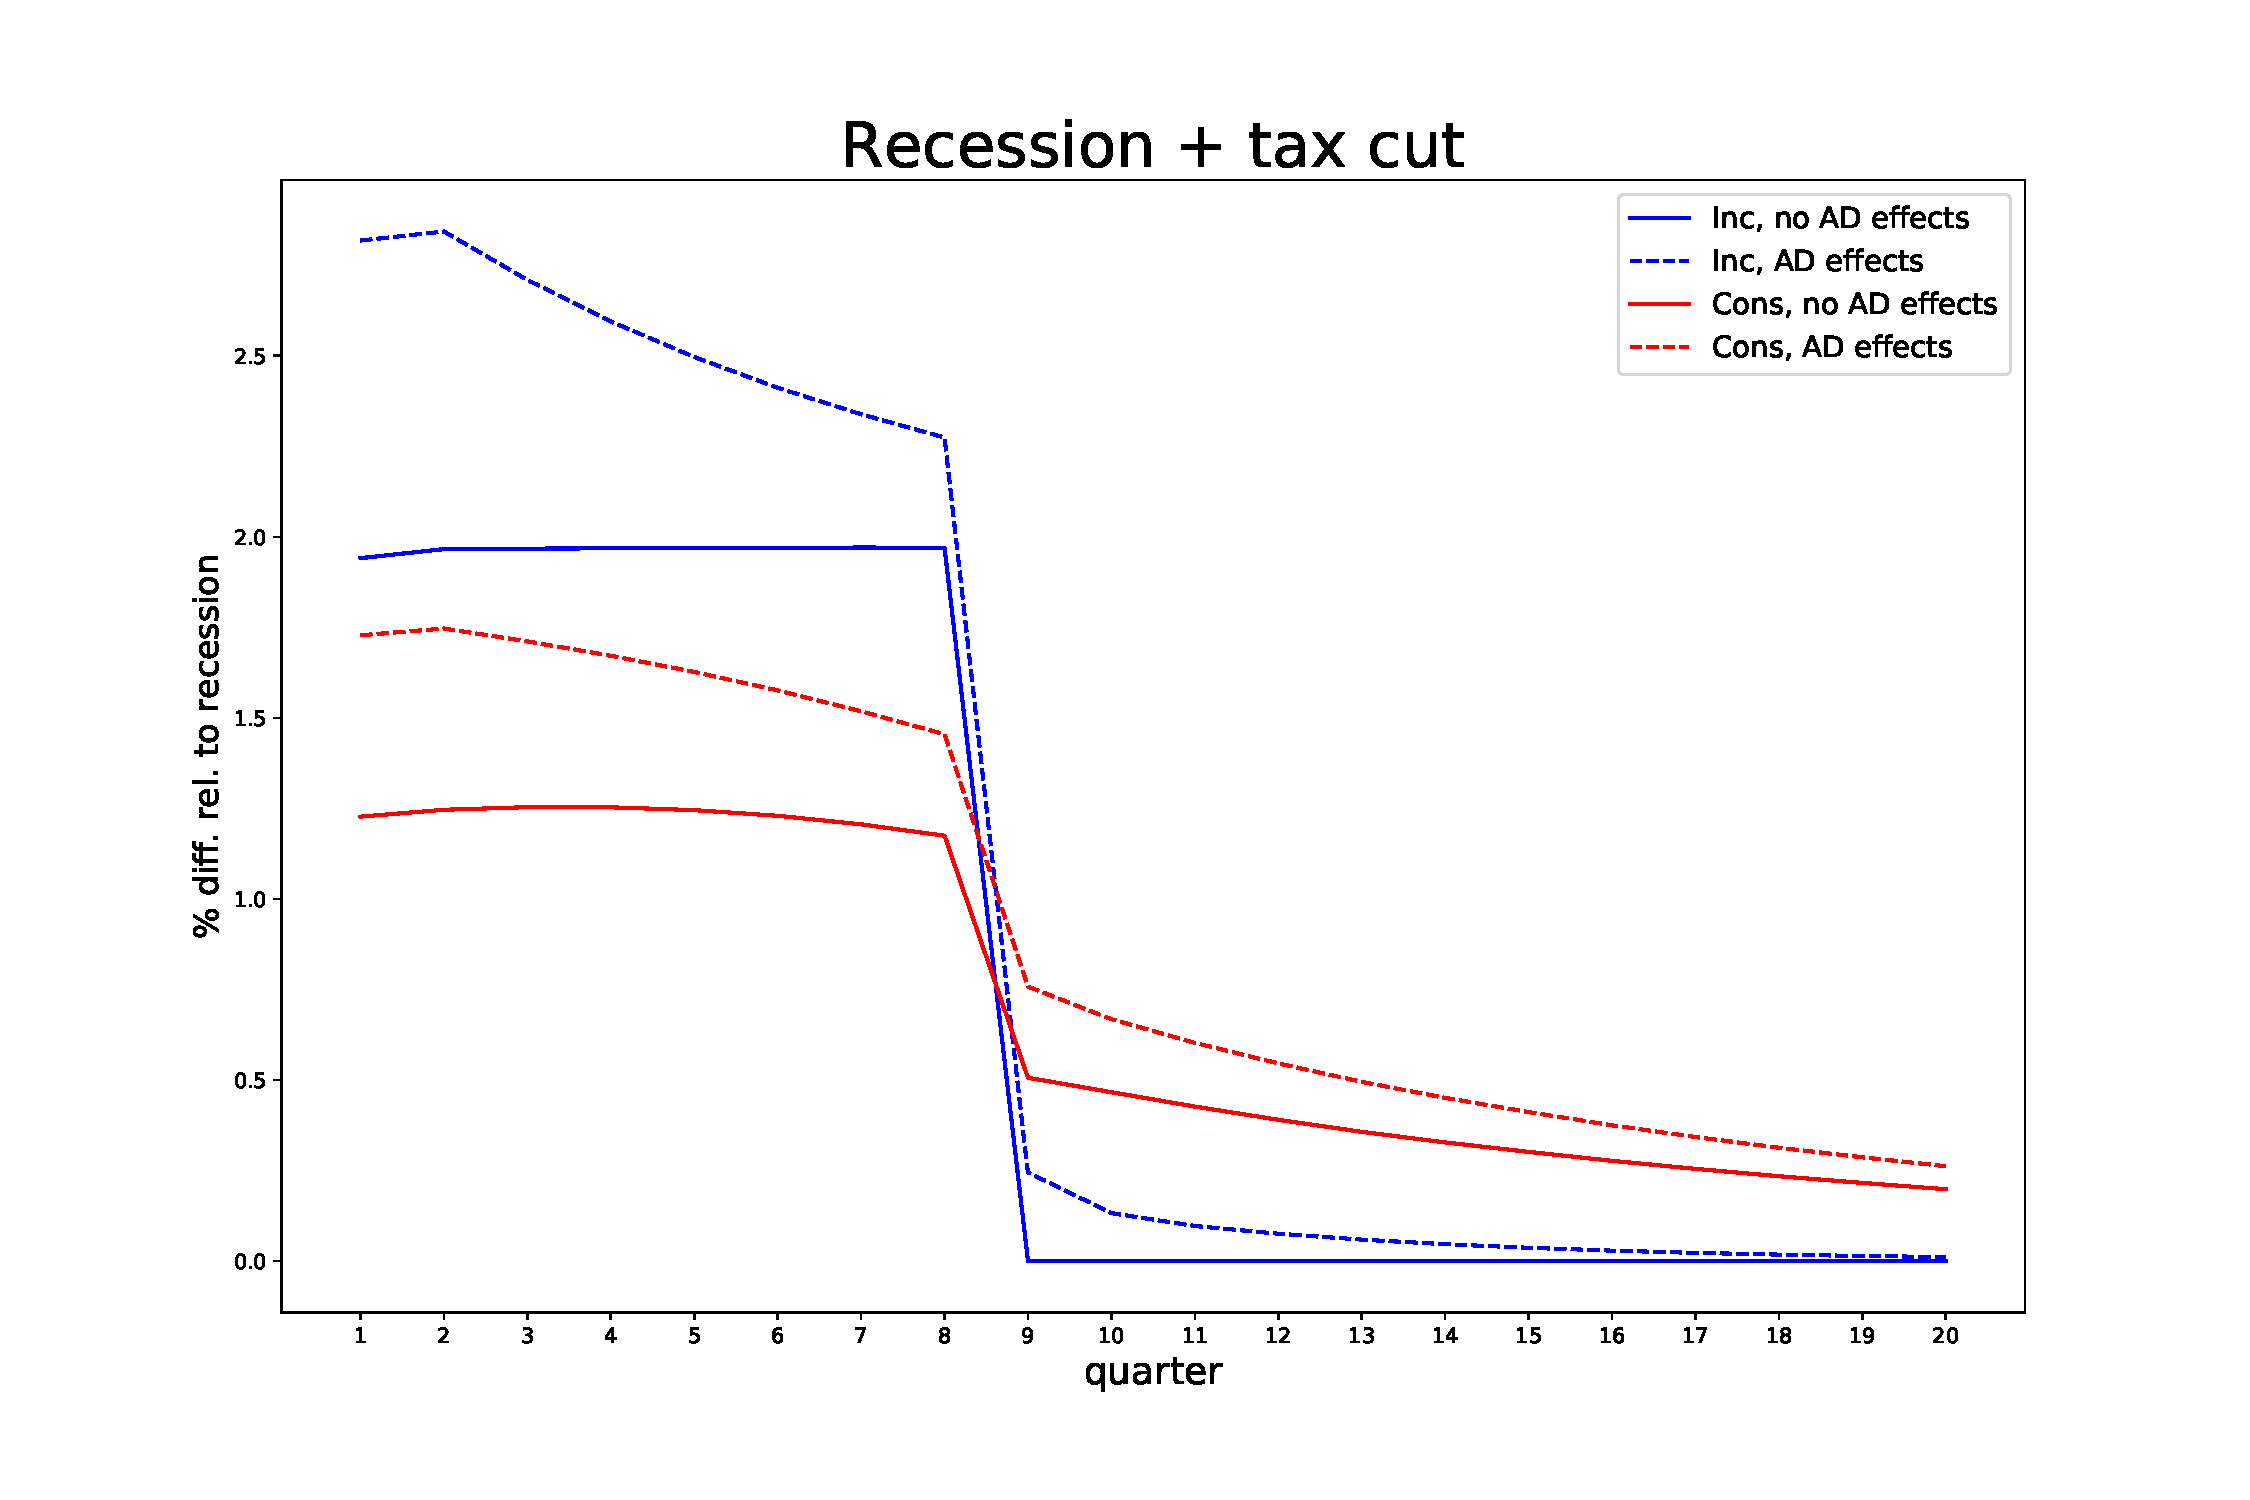
\includegraphics[width=\linewidth]{../FullRun_June7th/recession_taxcut_relrecession}
	\caption{}
	\label{fig:recessiontaxcutrelrecession}
\end{figure}

\begin{figure}
	\centering
	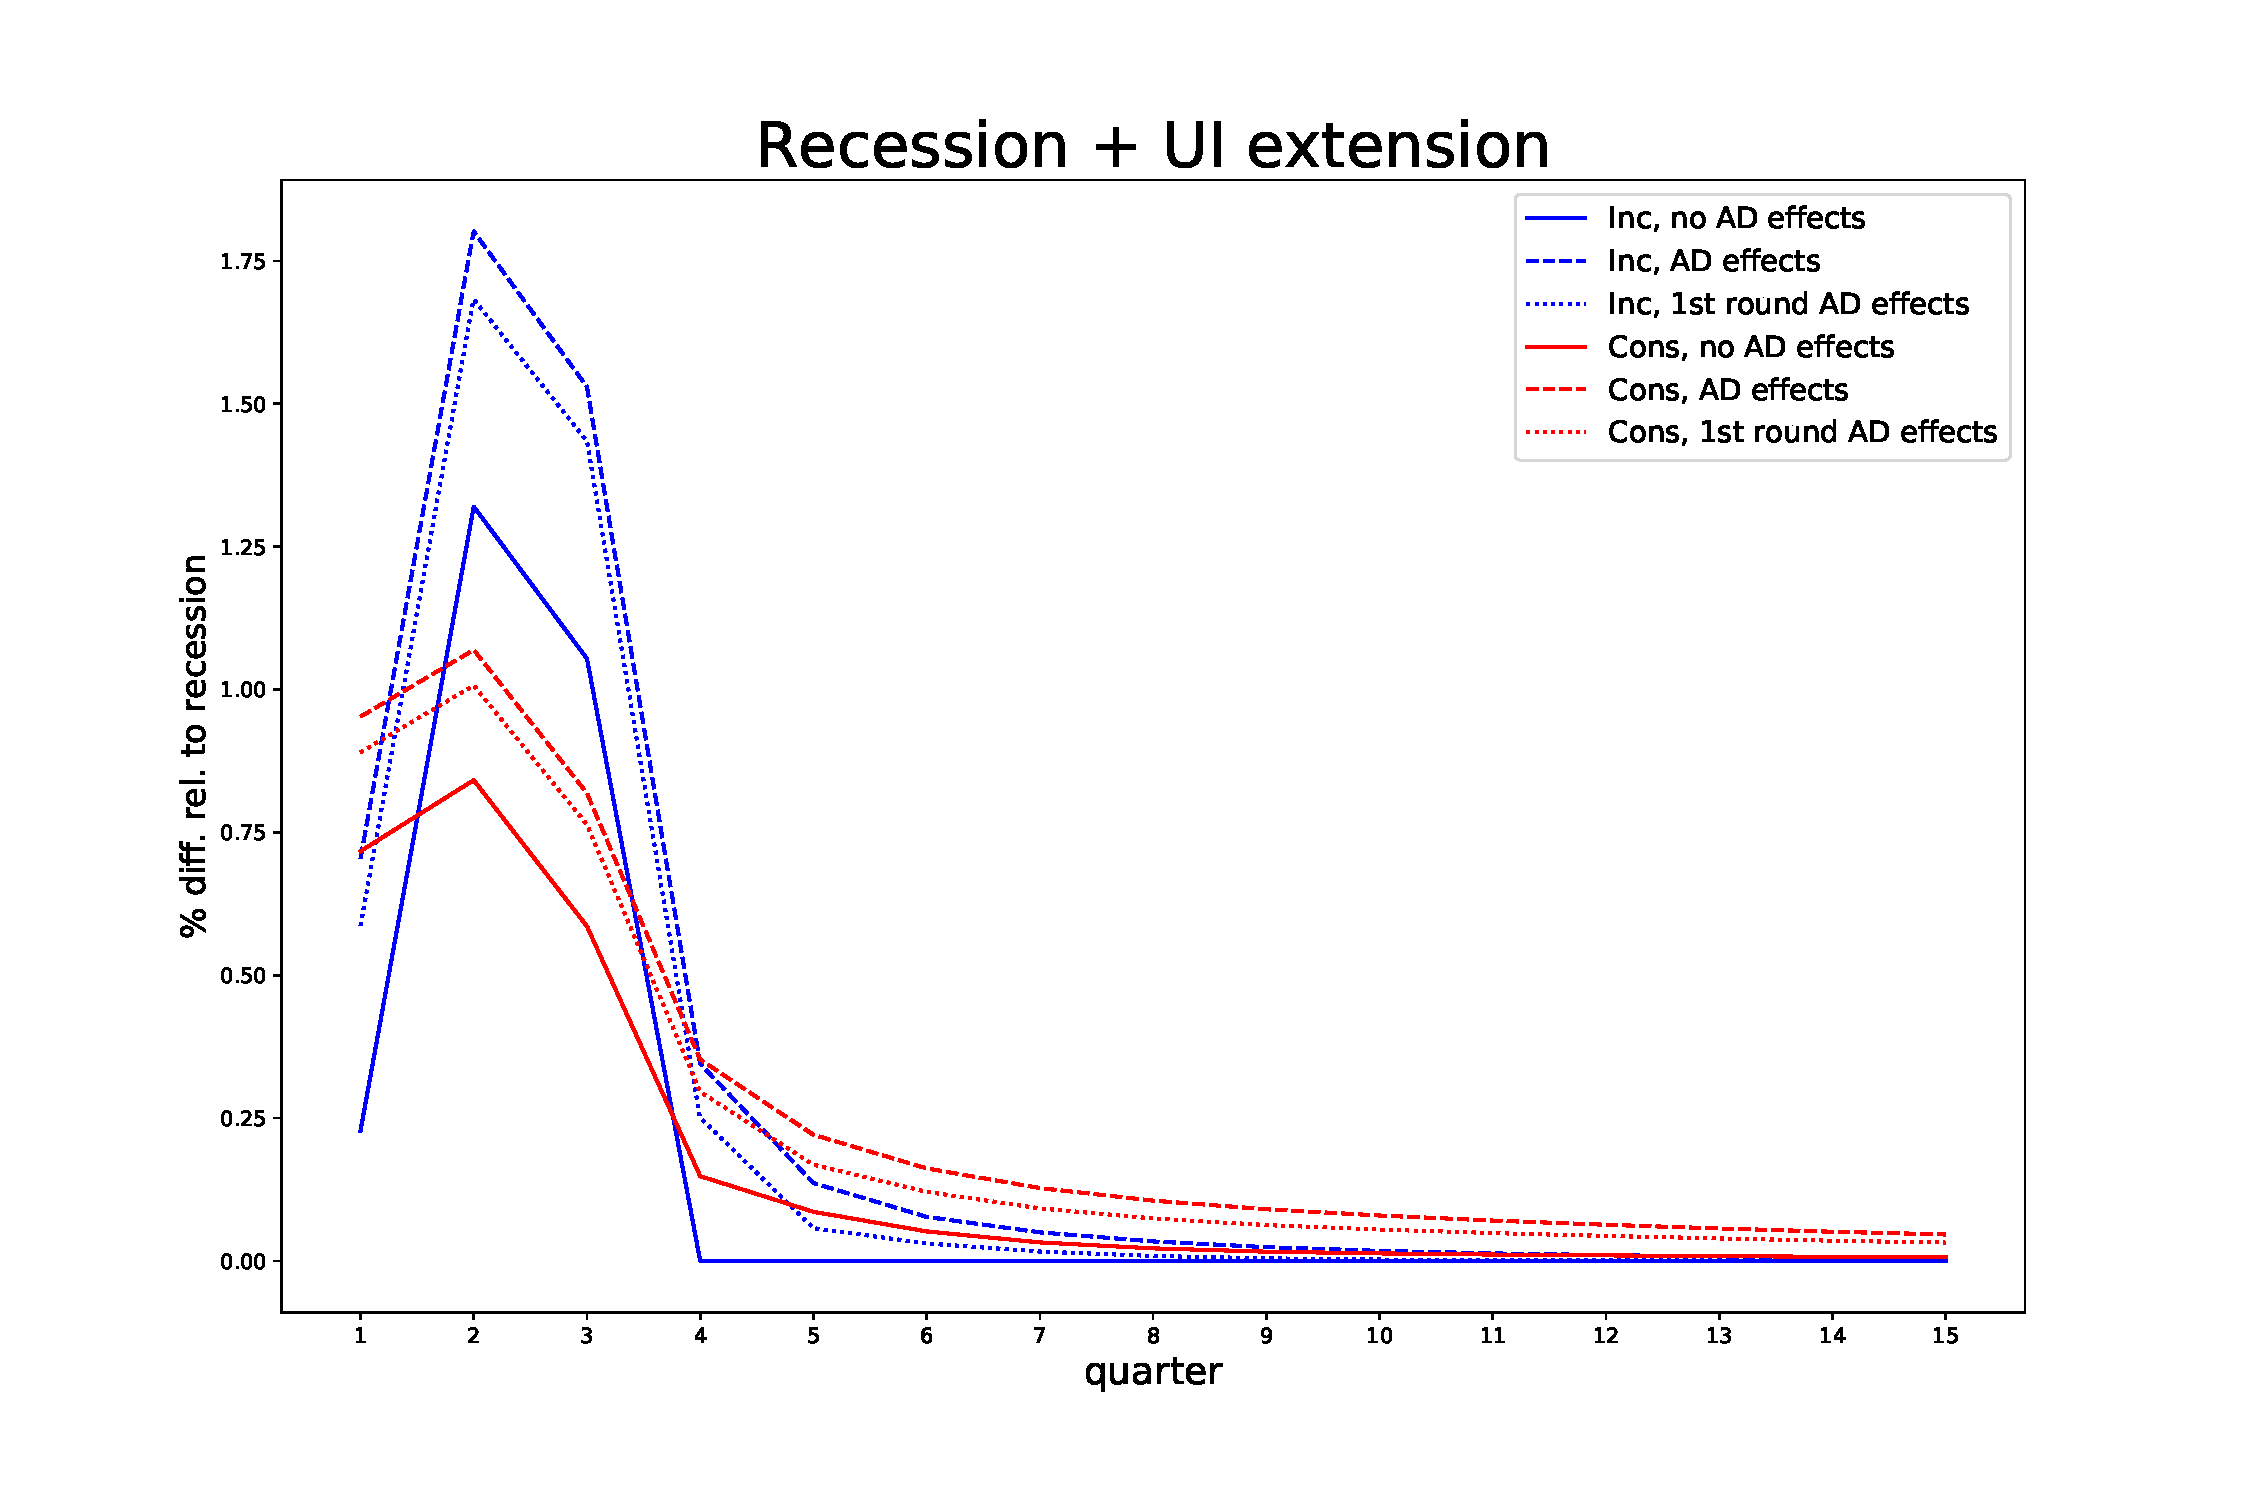
\includegraphics[width=\linewidth]{../FullRun_June7th/recession_UI_relrecession}
	\caption{}
	\label{fig:recessionuirelrecession}
\end{figure}

\begin{figure}
	\centering
	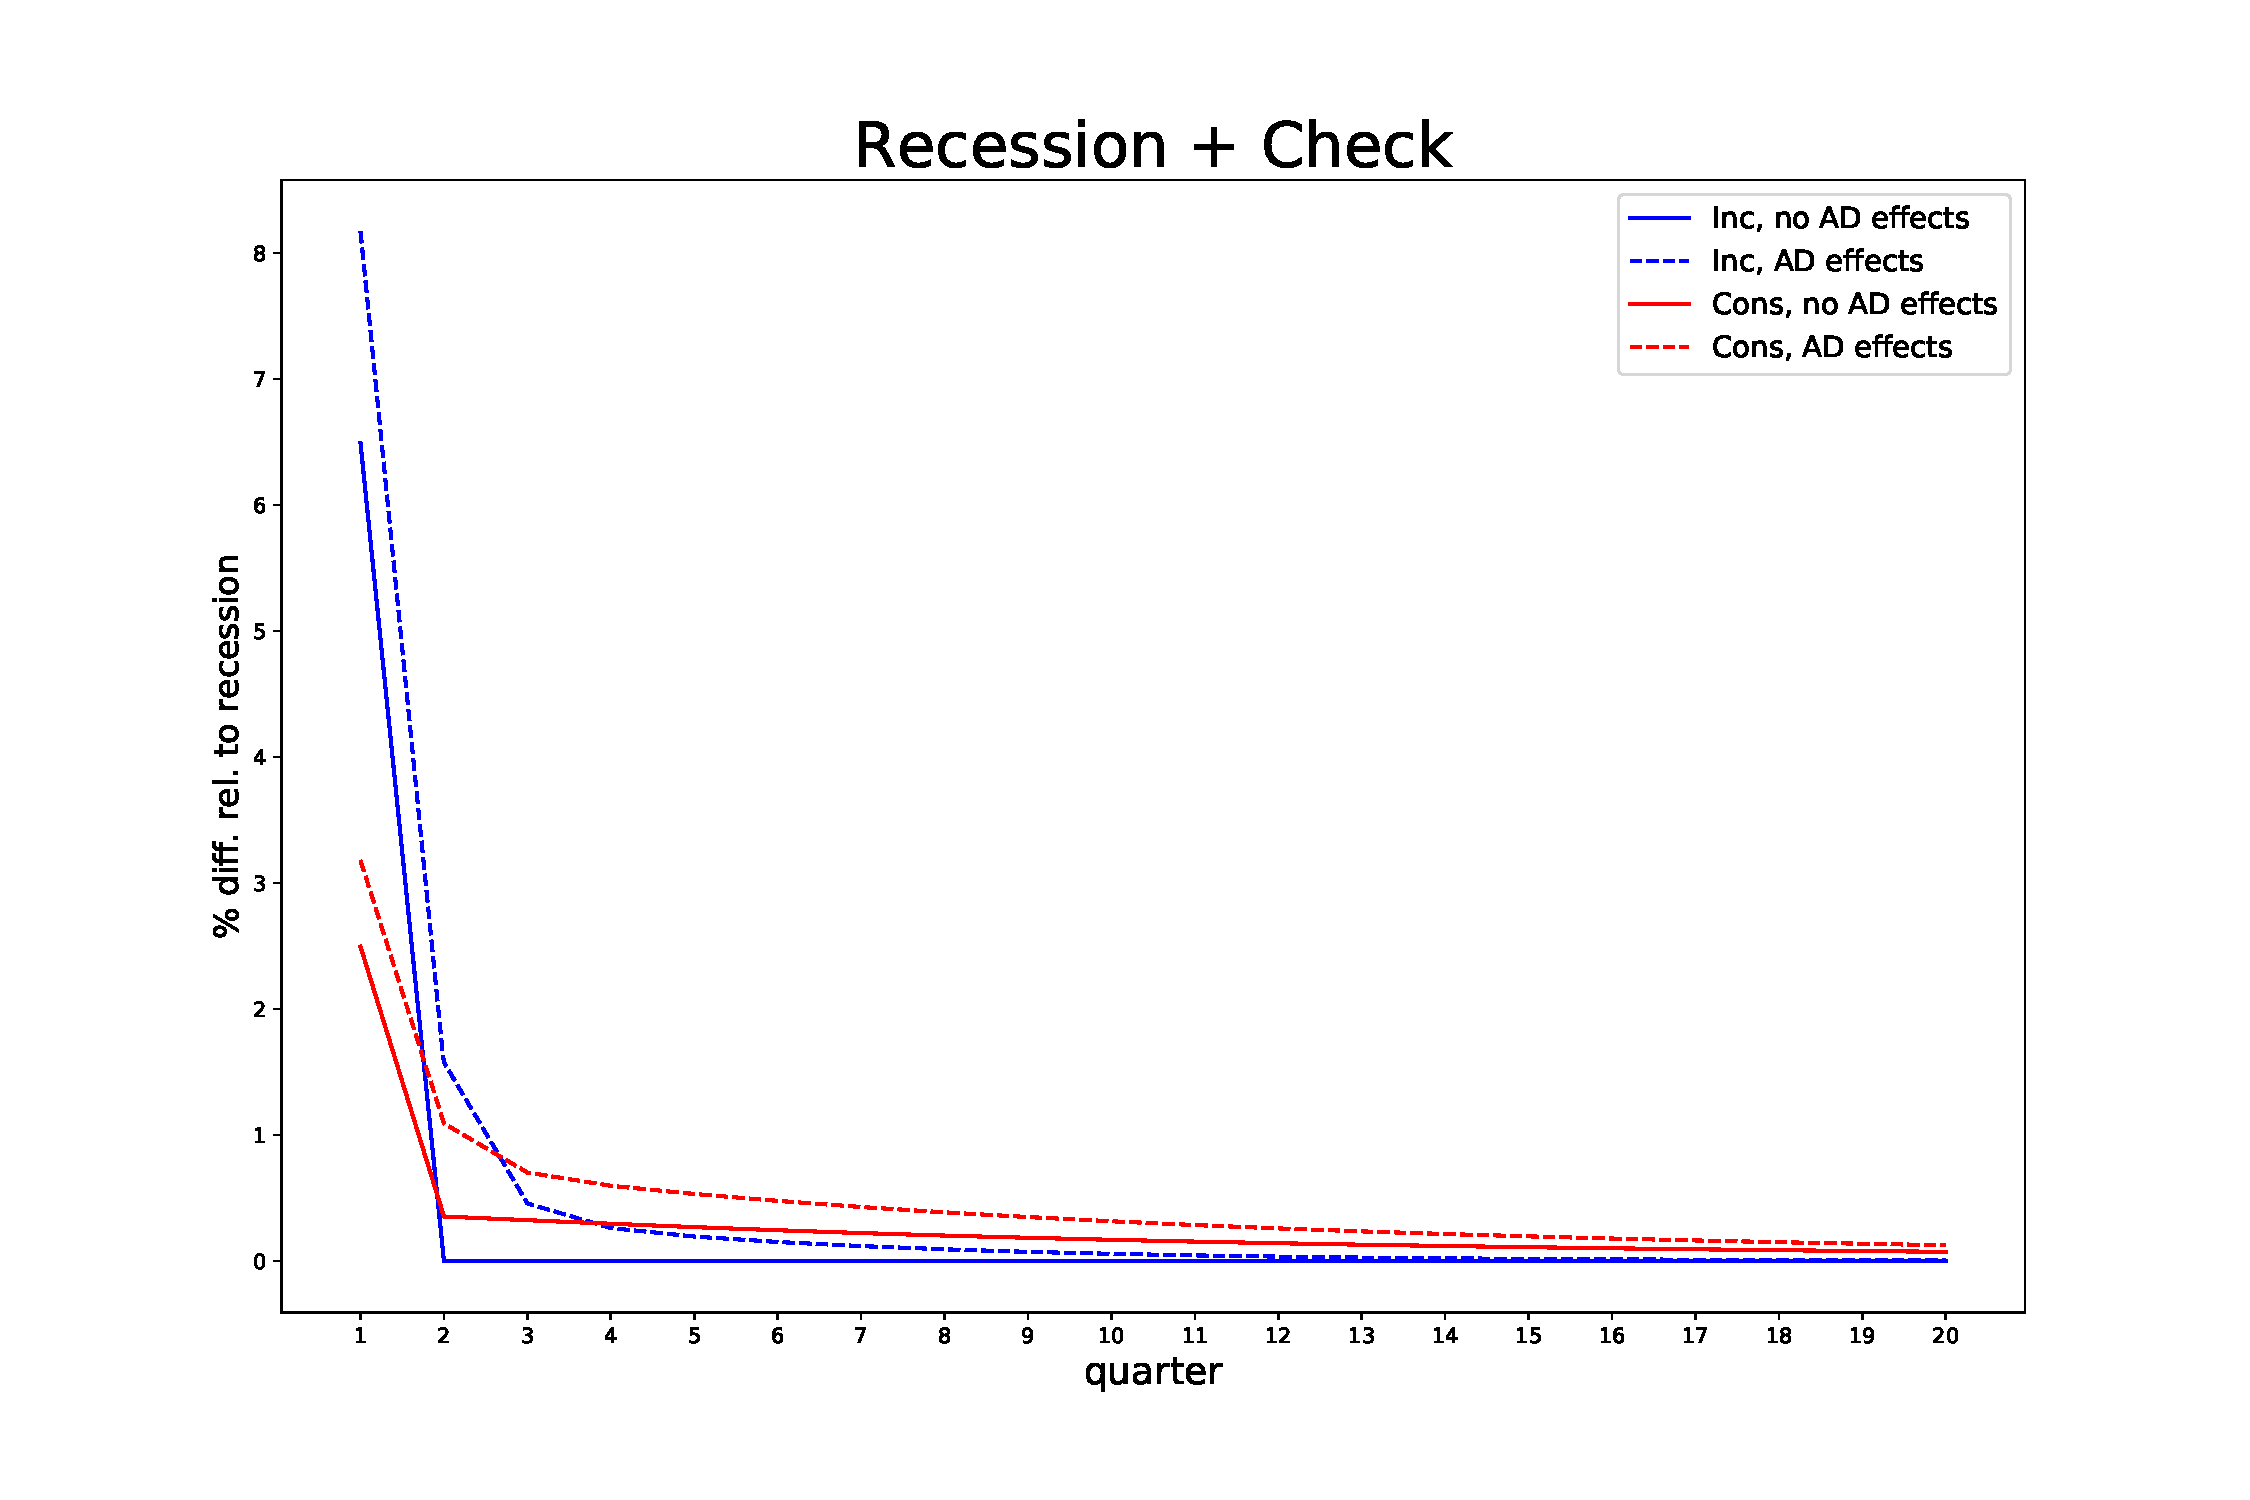
\includegraphics[width=\linewidth]{../FullRun_June7th/recession_Check_relrecession}
	\caption{}
	\label{fig:recessioncheckrelrecession}
\end{figure}


\FloatBarrier
\subsection{Multipliers}

We can look at three different multipliers

\begin{enumerate}
	\item Period multiplier: The ratio of additional consumption to policy expenditures at a certain point in time
	\begin{equation}
	PM(t) = \frac{\Delta C (t) }{\Delta G(t)}
	\end{equation}	
	where $\Delta X(t)$ is the difference in the variable $X$ between the no-policy and policy scenario at time $t$.
	
	\textit{Useful to investigate at which point in time a policy is most effective}
		
	\begin{figure}[h!]
		\centering
		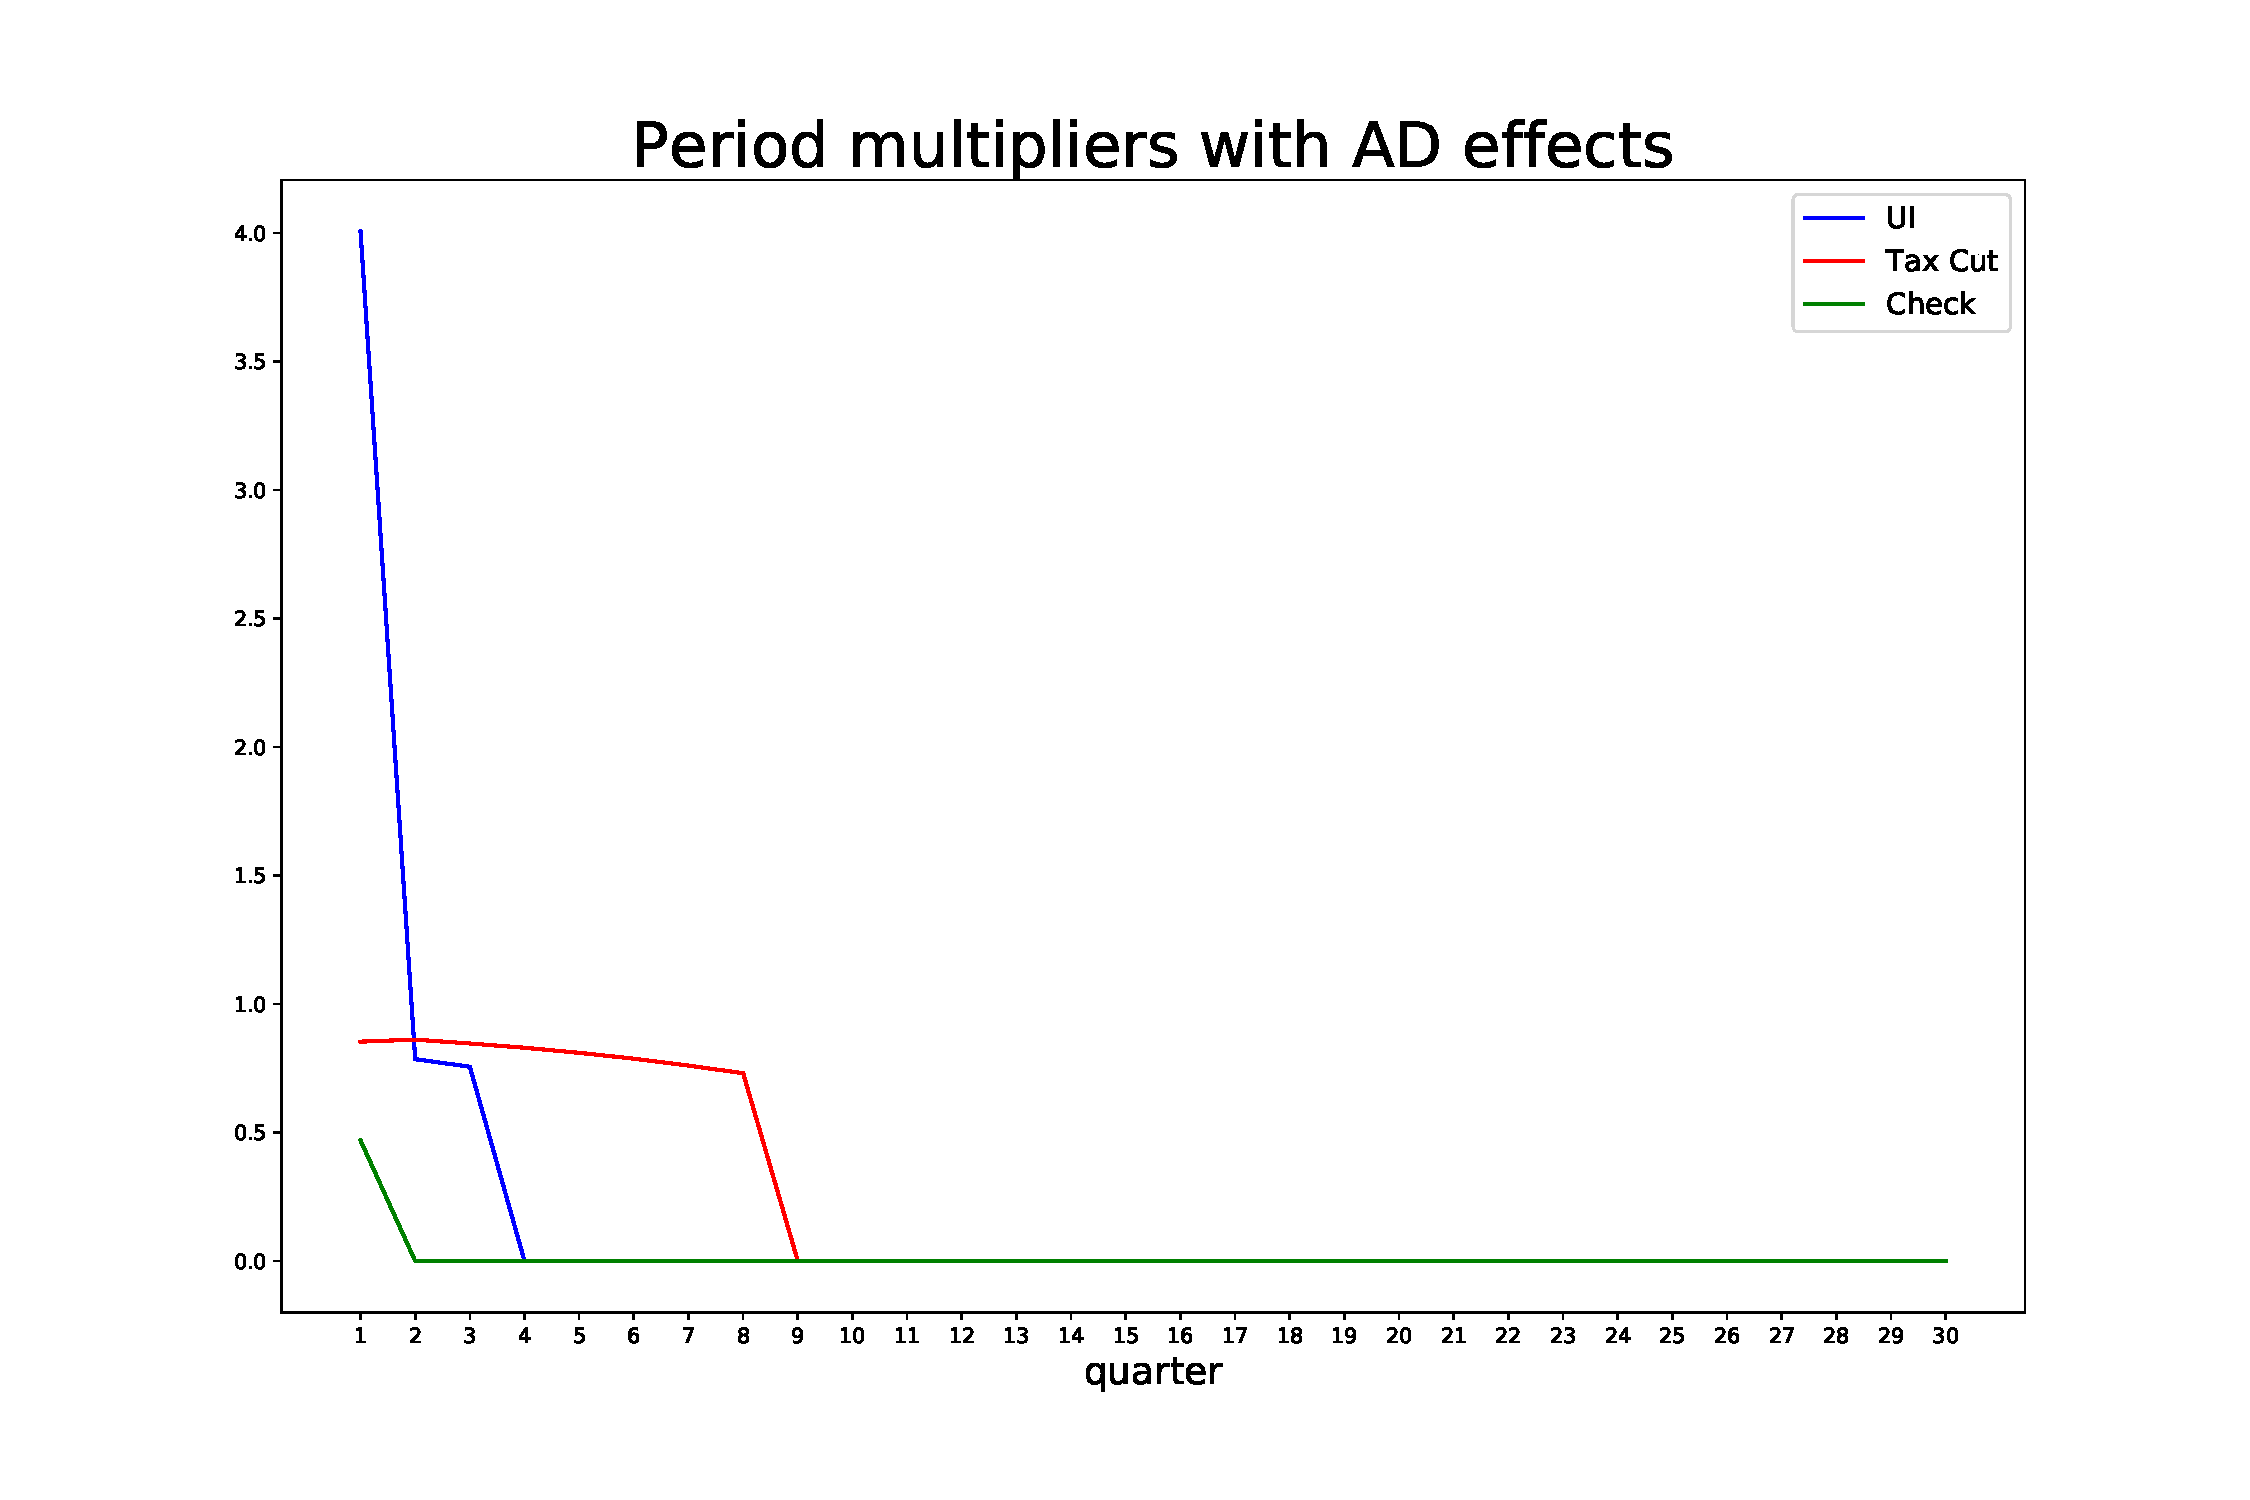
\includegraphics[width=\linewidth]{../FullRun_June7th/P_multipliers}
		\caption{}
		\label{fig:pmultipliers}
	\end{figure}
	
	\item Net present value multiplier: The ratio of the NPV of additional consumption to the NPV of policy expenditure up to a certain point in time.
	\begin{equation}
	NPVM(t) = \frac{NPV(t,\Delta C)}{NPV (t,\Delta G)}
	\end{equation}	
	where the net present value of a variable X at horizon t is given by
	\begin{equation}
	NPV(t,X) = \sum_{s=0}^{t} \left( \prod_{i=1}^{s} \frac{1}{R_i} \right) X_s
	\end{equation}
	
	\textit{Useful to investigate at which horizons the policy becomes effective}
	
	\begin{figure}
		\centering
		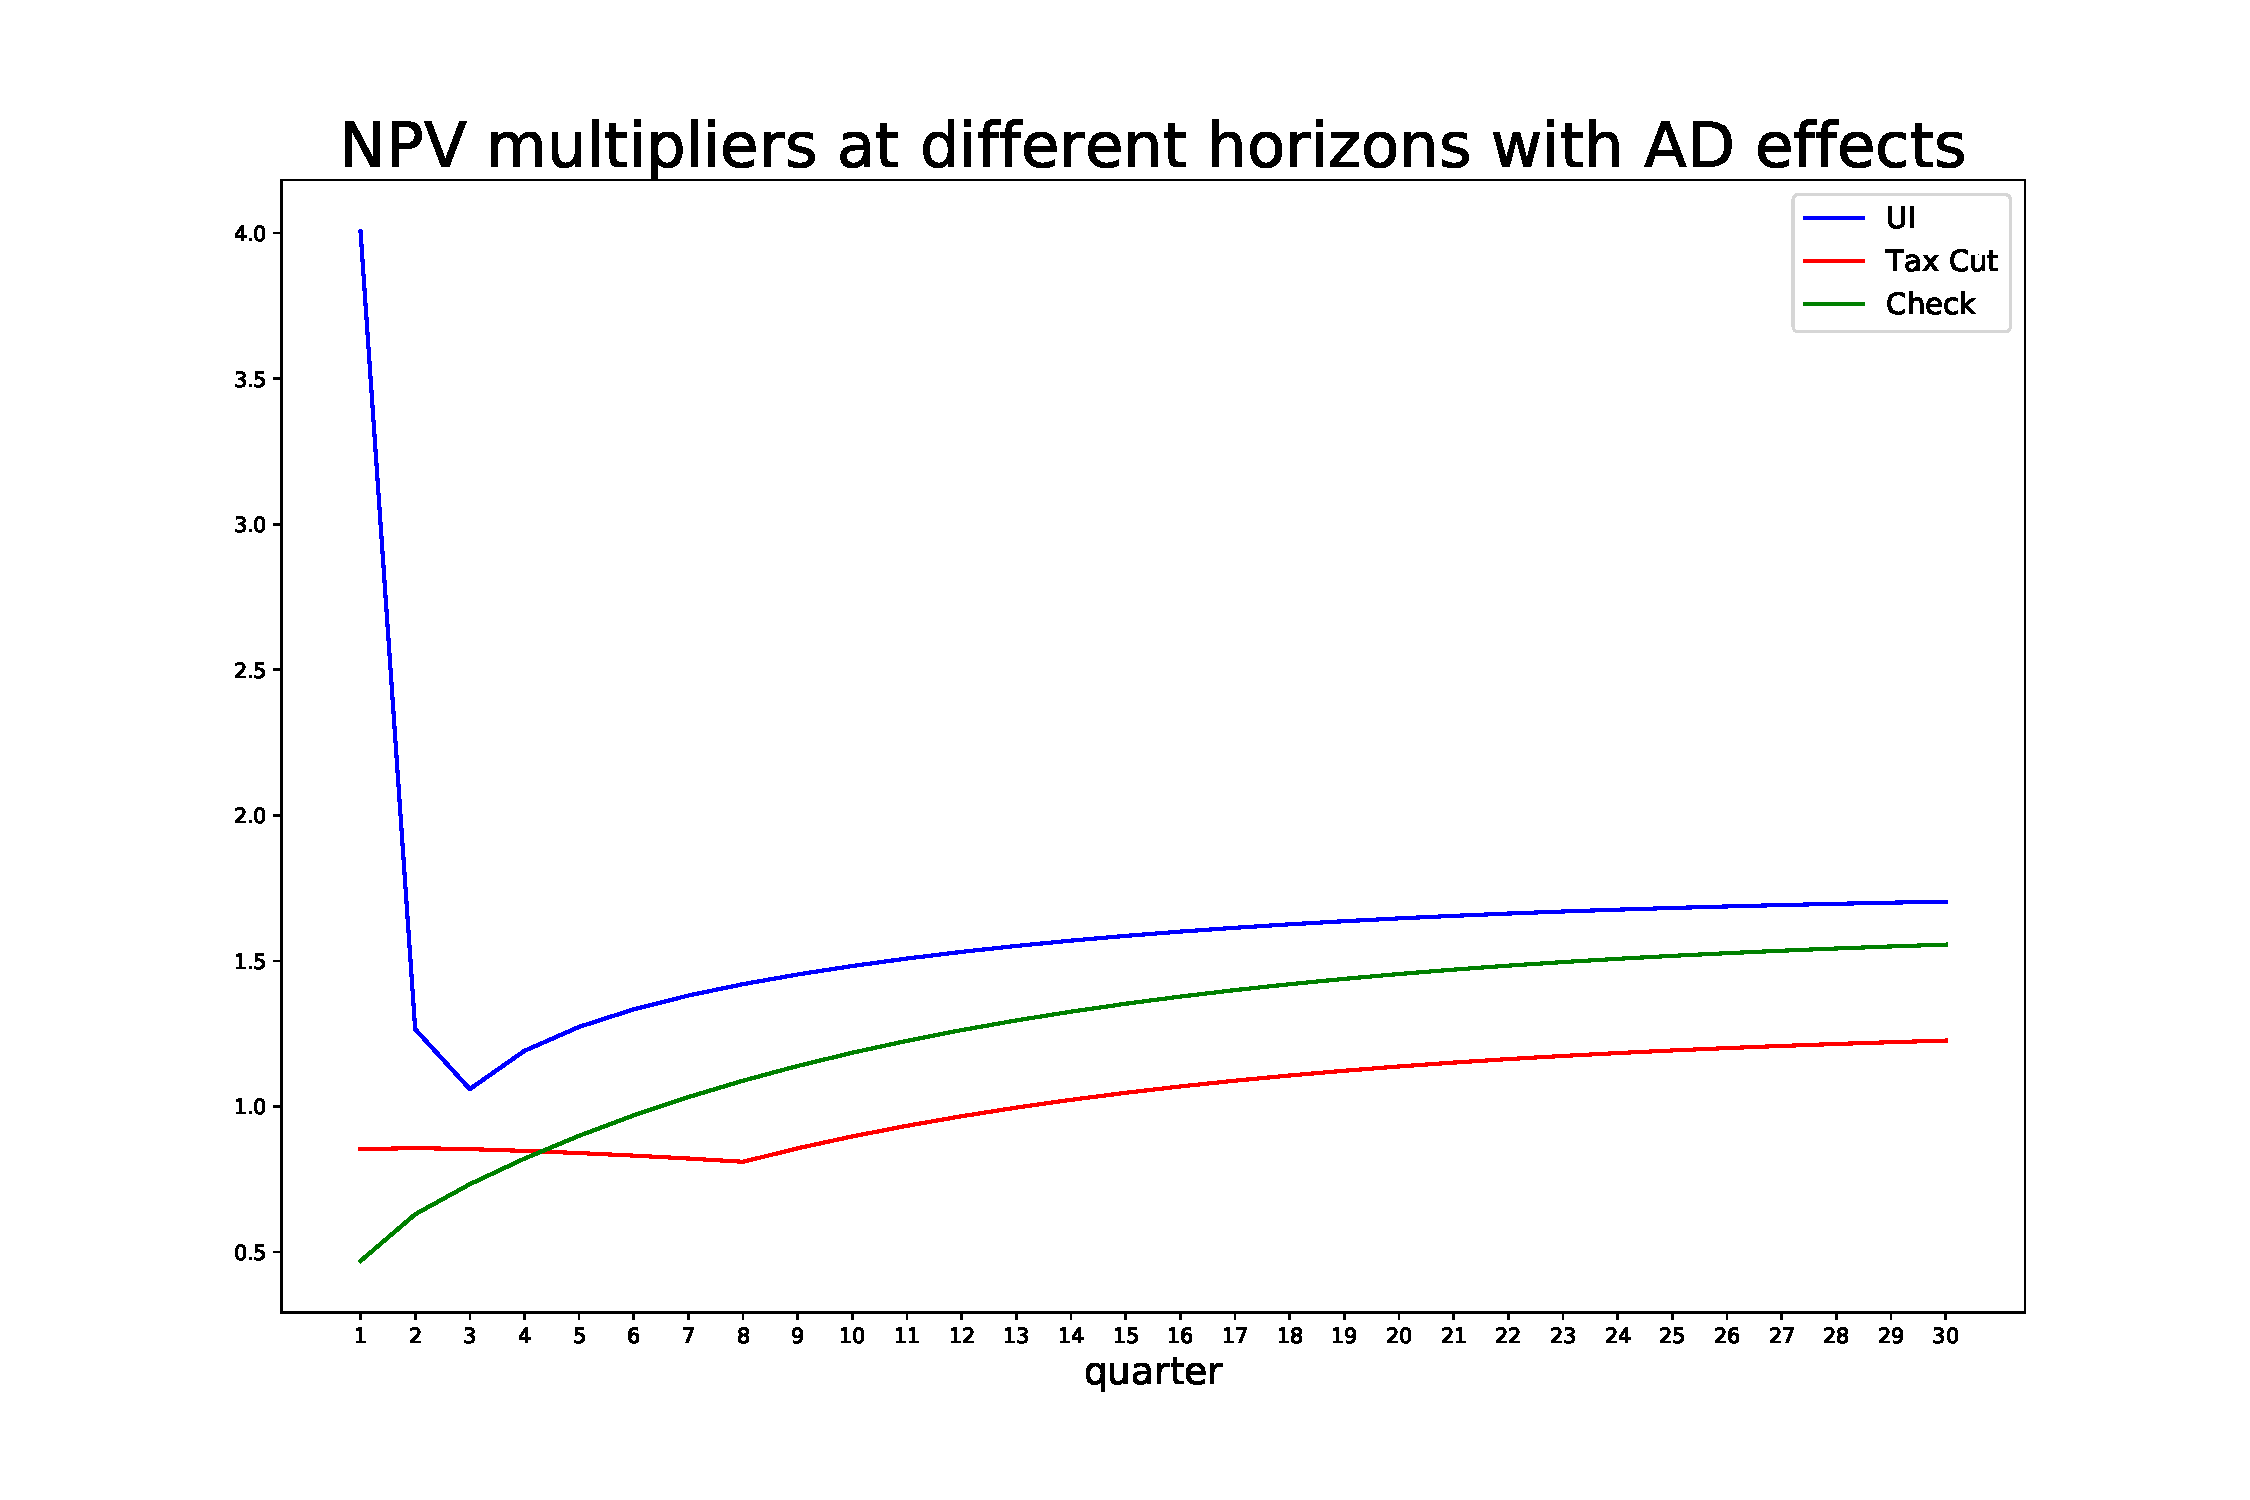
\includegraphics[width=\linewidth]{../FullRun_June7th/NPV_multipliers}
		\caption{Net present value multipliers at horizon 1 (impact multiplier) to 30}
		\label{fig:npvmultipliers}
	\end{figure}
	
	
	\item Cummulative multiplier: The ratio of the NPV of additional consumption up to time $t$ to the infinite-horizon NPV of policy expenditure
	\begin{equation}
	CM(t) = \frac{NPV(t,\Delta C)}{NPV (\infty,\Delta G)}
	\end{equation}
	
	\textit{Useful to investigate when additional consumption occurs}
	
	\begin{figure}
		\centering
		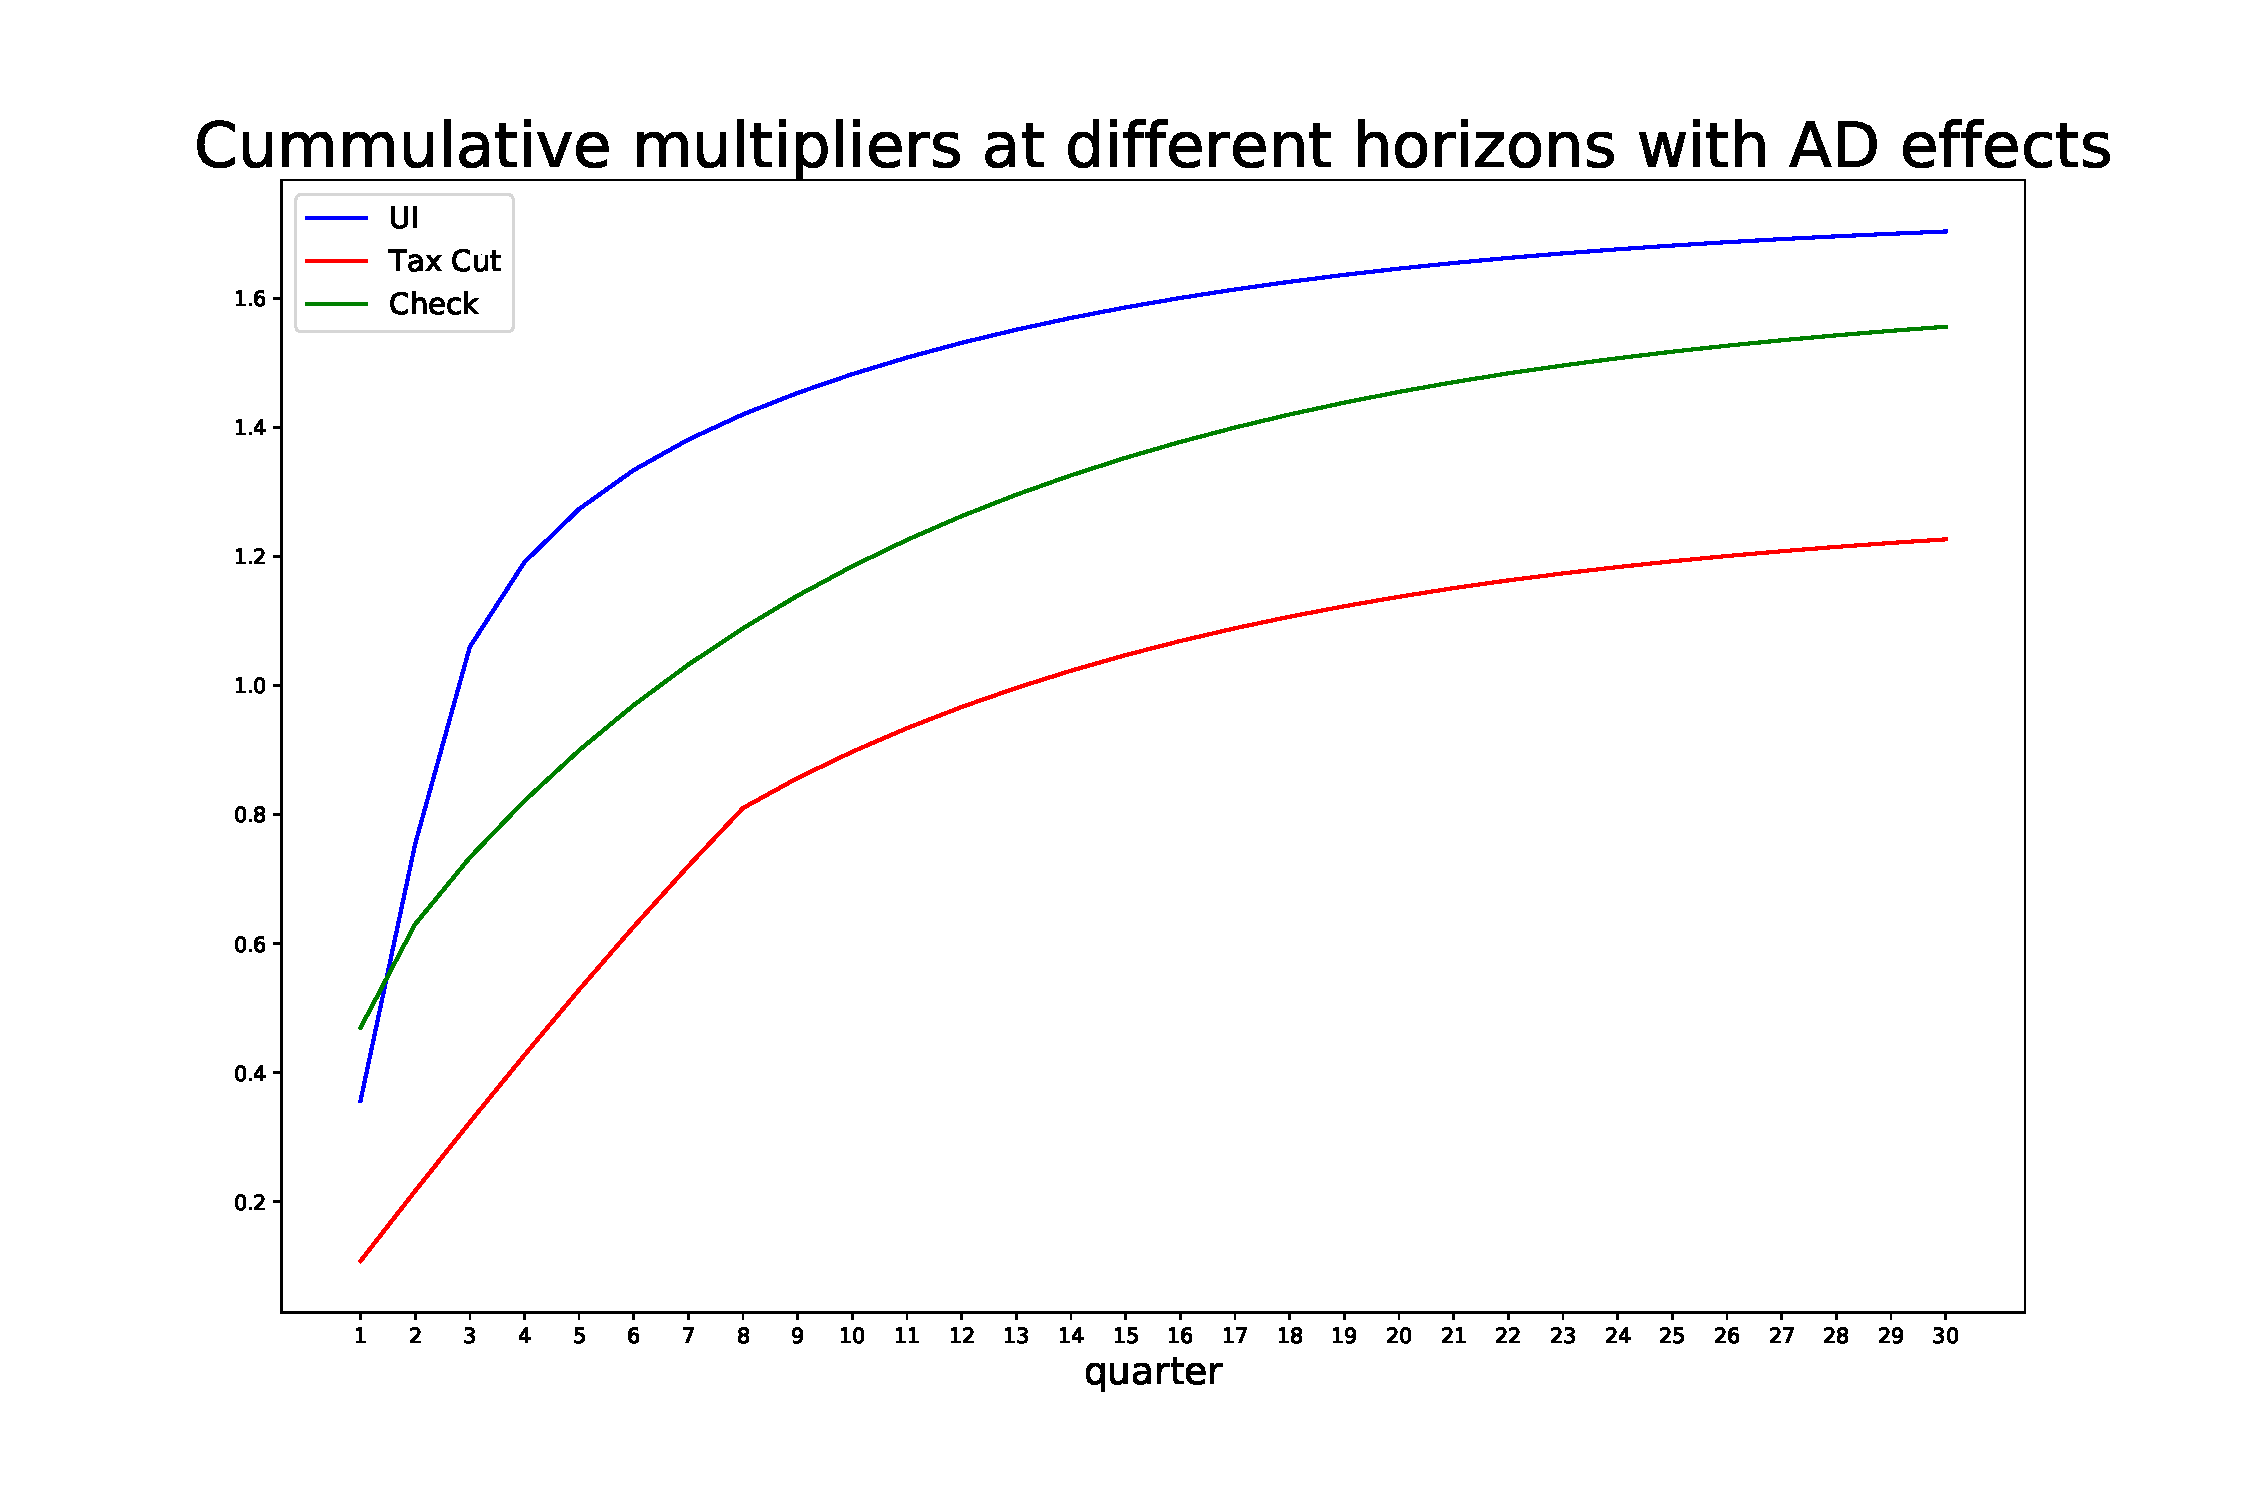
\includegraphics[width=\linewidth]{../FullRun_June7th/C_multipliers}
		\caption{}
		\label{fig:cmultipliers}
	\end{figure}
	
\end{enumerate}









	


\FloatBarrier
\subsection{Long-run NPV multipliers table}

The table shows $NPVM(\infty)$.

\begin{table}[htb]
	\centering
	\begin{tabular}{@{}llllll@{}}
		\toprule
		Experiment  	& no AD effects & AD = 0.5 		& AD = 0.5 (1st round)	& AD = 0.25 	& AD = 0.75 	\\ \midrule
		Payroll tax cut & 1 			& 1.28   		& 1.18  			    & 1.10			& 1.58			\\
		UI extension    & 0.98 			& 1.74 			& 1.51 					& 1.30			& 2.42			\\
		Check		    & 0.97 			& 1.62 			& 1.40 					& 1.23			& 2.25			\\ \bottomrule
	\end{tabular}	
	\caption{Long-run multipliers}
\end{table}


	

\begin{comment}


\section{Update - May 19th 2021}

\begin{figure}
	\centering
	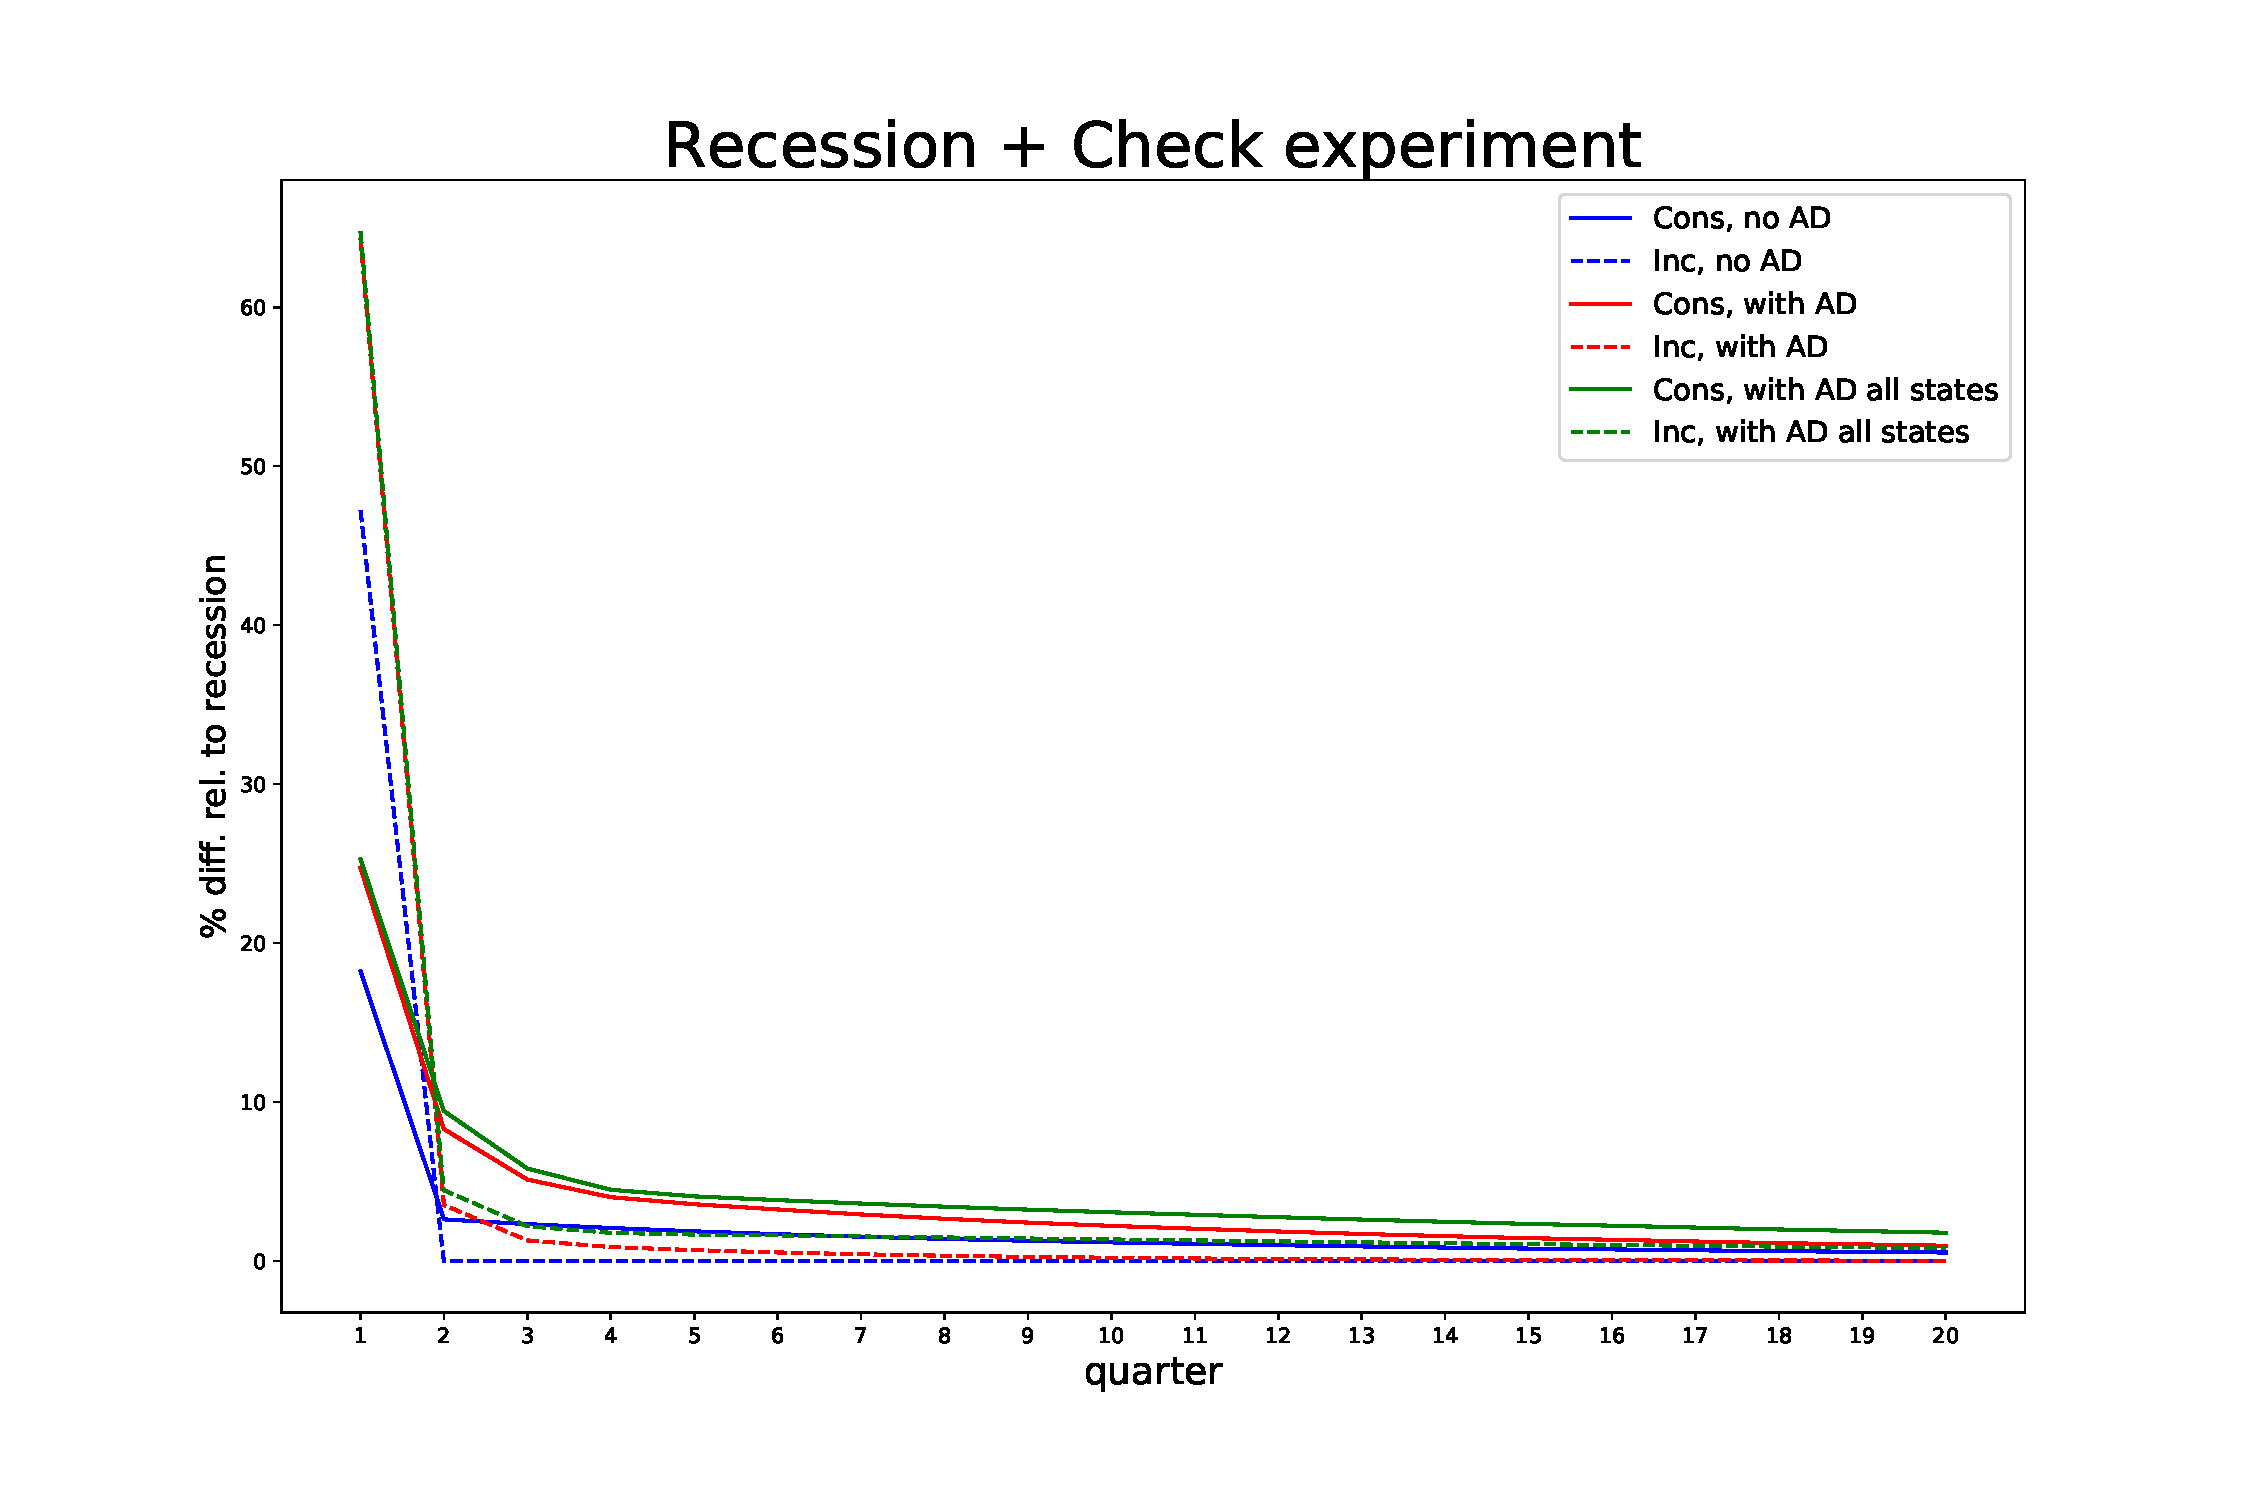
\includegraphics[width=\linewidth]{../Check_Experiment/recession_Check_relrecession}
	\caption{One period stimulus check}
	\label{fig:recessioncheckrelrecession}
\end{figure}

\begin{itemize}
	\item Figure \ref{fig:recessioncheckrelrecession}: The stimulus check has the size 0.5 x the mean permanent income level (which is set to 1 in the code). 
	\item Everyone up to a first income threshold (again expressed ad multiple of the mean permanent income) receives 100 \% of the check (and within this group everyone gets the same amount), everyone above a second threshold 0 \% of the check size, and everyone inbetween a proportion according to the linear distance between these two threshold points.
	\item Income on average thus increases slightly below 50 \% because some of the richer agents don't get the check fully or at all.
	The stimulus check goes to everyone to 100 \% up to a first
	\item AD effects increase income, AD effects even during non-recession states increase income even more 
	\item Figure \ref{fig:npvmultirecessioncheckrelrecession} shows the NPV multiplier for different time-horizons. The multipliers reach, after 80q a long-run multiplier of 0.97 (no AD effects), 1.70 (with AD effects) and 2.24 (with AD effects in all states).
\end{itemize}


\begin{figure}
	\centering
	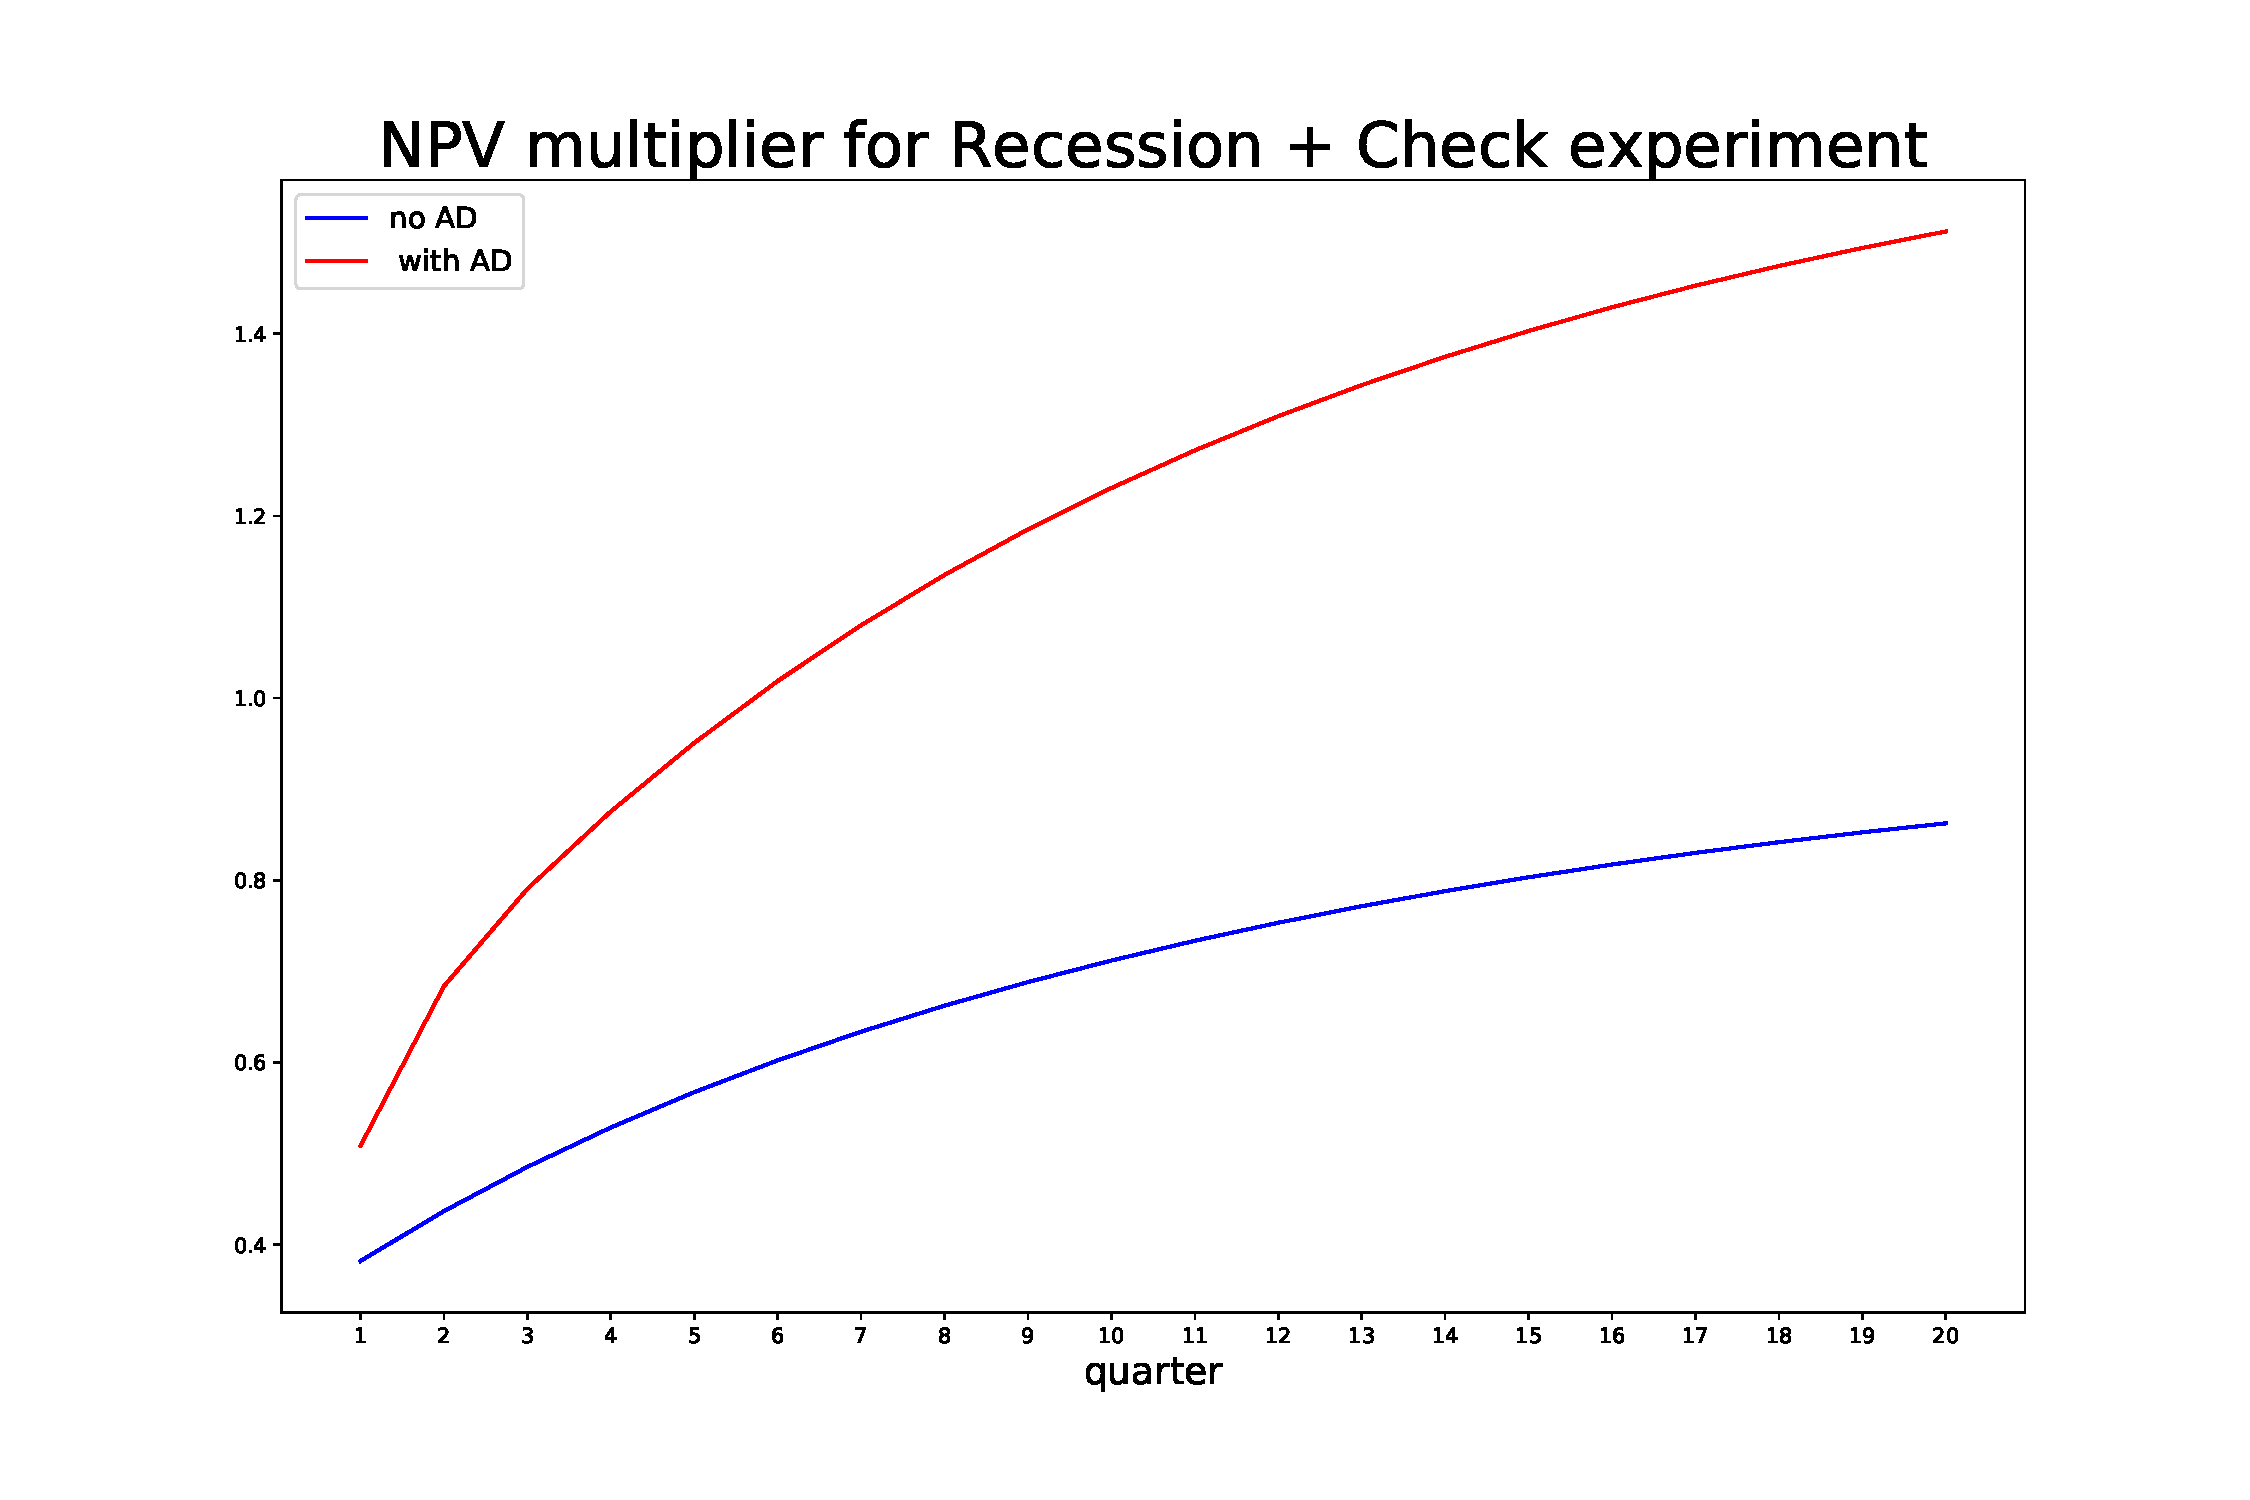
\includegraphics[width=\linewidth]{../Check_Experiment/NPVmulti_recession_Check_relrecession}
	\caption{}
	\label{fig:npvmultirecessioncheckrelrecession}
\end{figure}


\FloatBarrier	
\section{Update - Apr 21st 2021}

\subsection{Multipliers}
\begin{table}[htb]
	\centering
	\begin{tabular}{@{}llll@{}}
		\toprule
		Experiment  	& no AD effects & AD only in Rec. states 	& AD in all states \\ \midrule
		Payroll tax cut & 1 			& 1.3   			& 2.0  \\
		UI extension    & 1 			& 1.9 				& 2.7     \\ \bottomrule
	\end{tabular}	
	\caption{Long-run multipliers for each policy intervention }
\end{table}
	
Difference to last update: Only the number 2.7 has increased (from 2.2). Reason is that simulation now has 800 k agents, as opposed to 200k


\FloatBarrier
\subsection{Multipliers under different recession / policy lengths}
\begin{figure}[h]
	\centering
	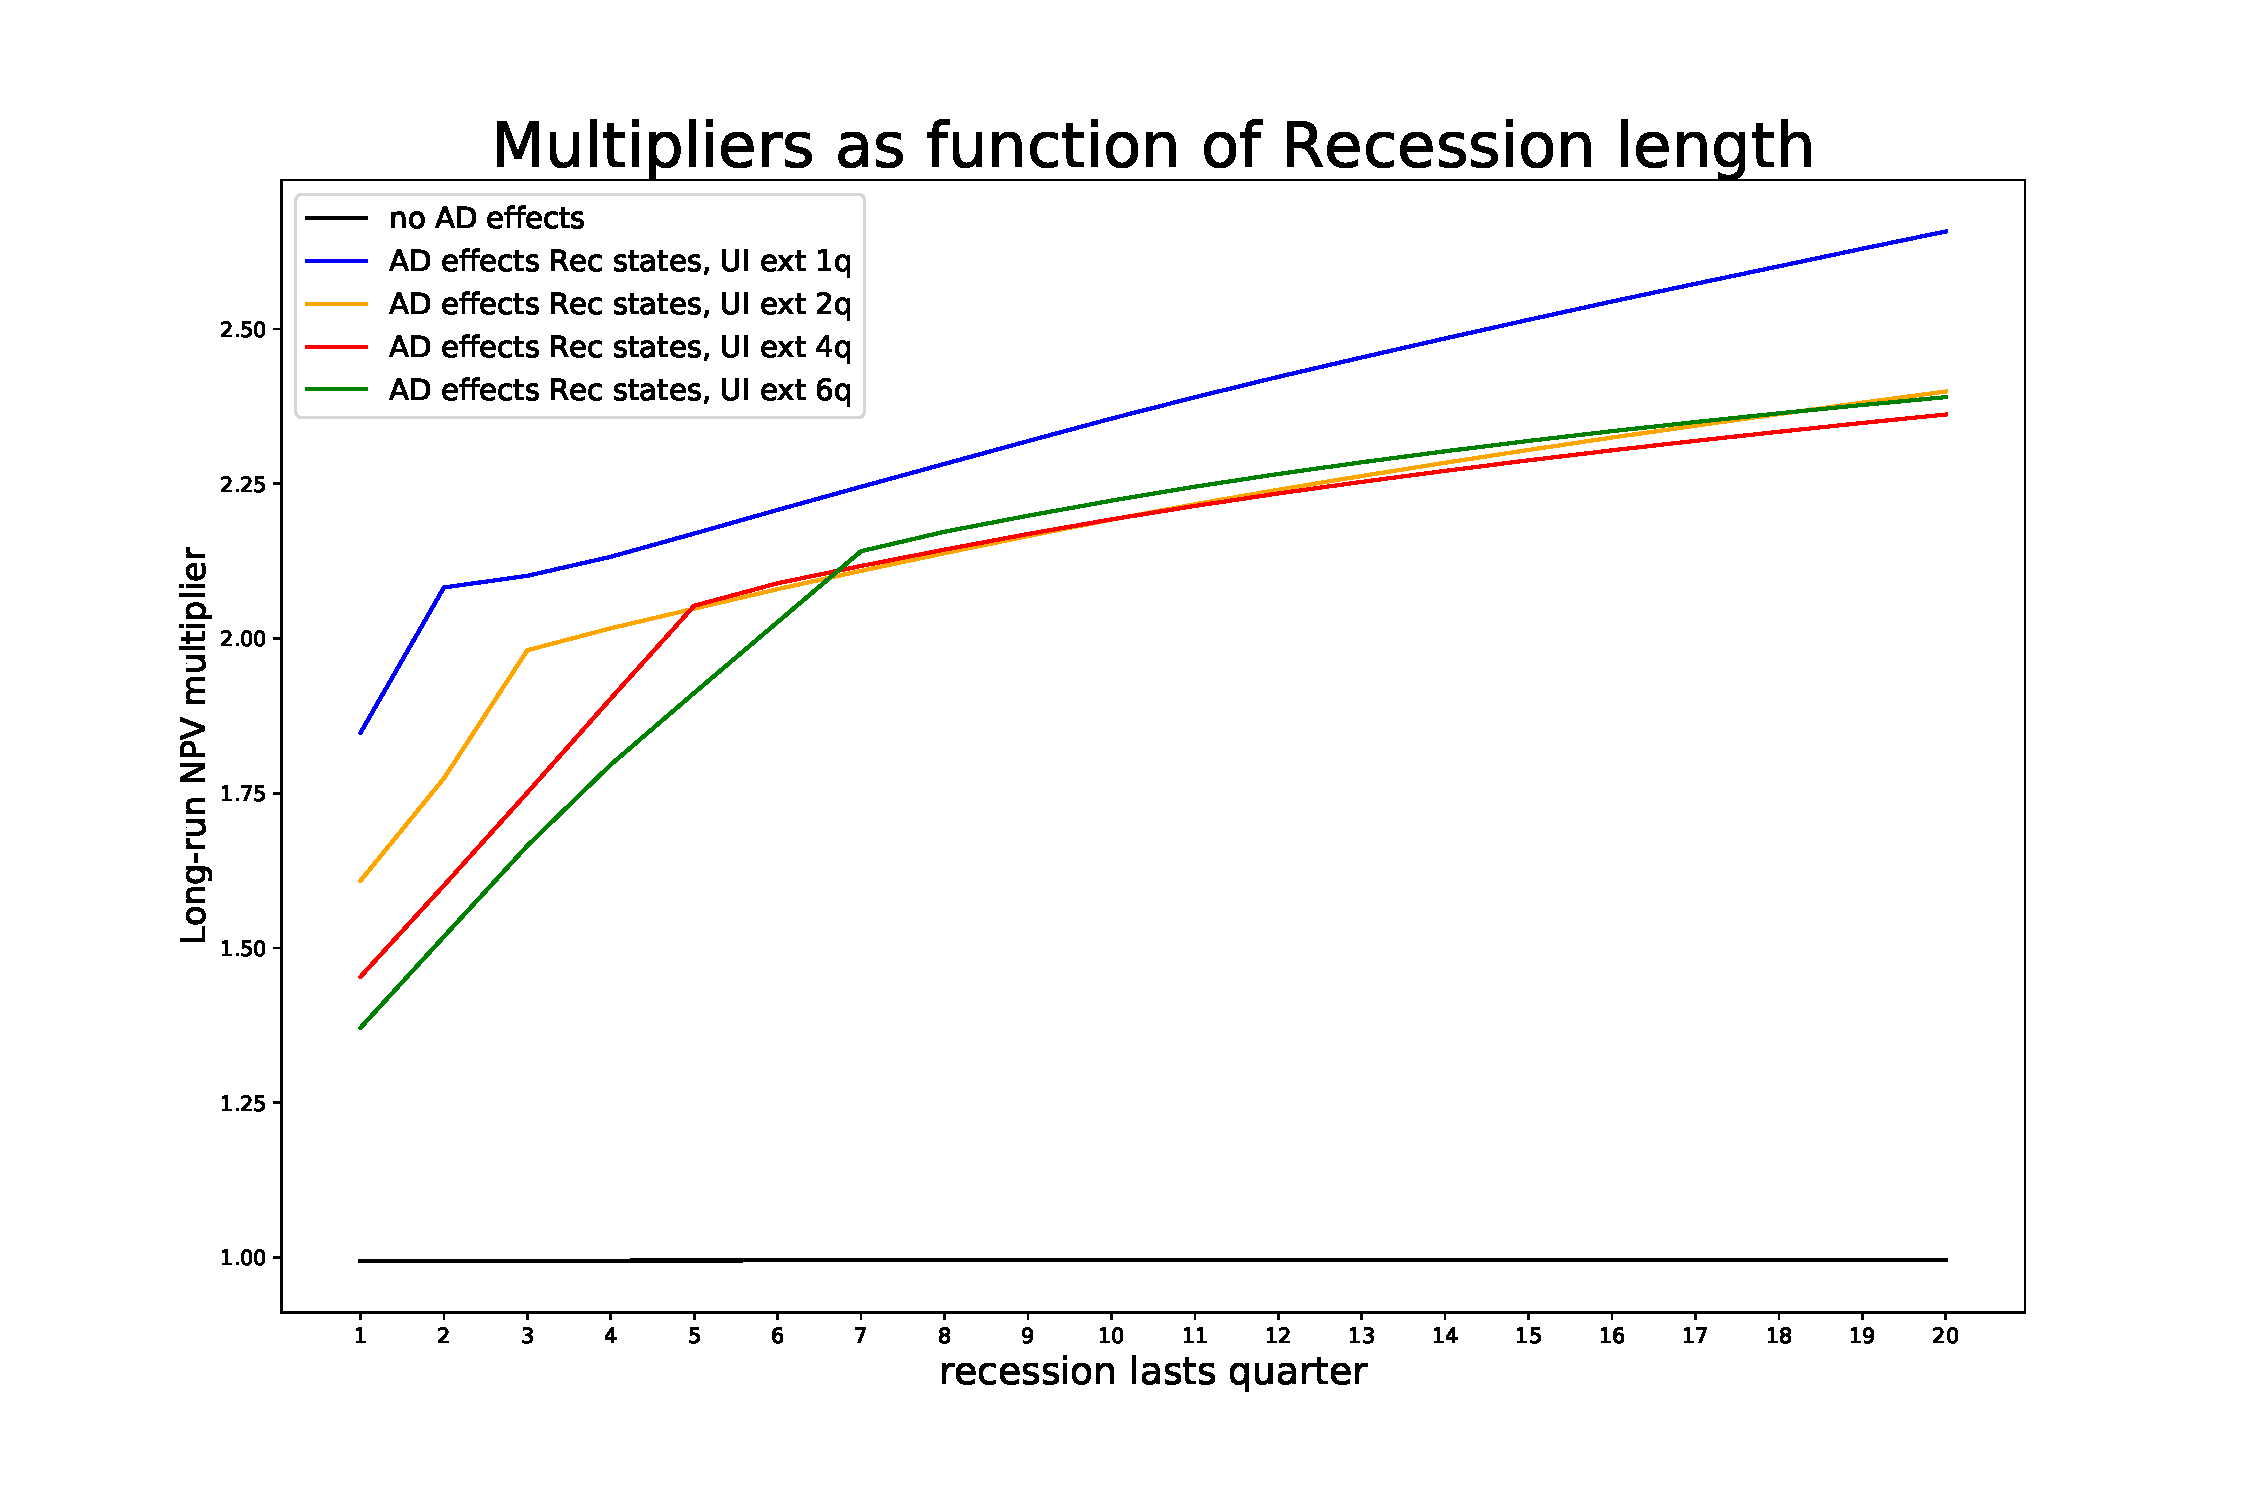
\includegraphics[width=1\linewidth]{../FullRun_Apr18_AD05_AllStates_800k/Multipliers_RecLength_PolicyLength1}
	\caption{}
	\label{fig:multipliersreclengthpolicylength1}
\end{figure}

\begin{enumerate}
	\item The longer the recesssion the higher the mulitplier, because of AD effects
	\item For short recessions: the shorter the UI extension in length, the higher the multiplier. Reason: 
	i) A higher share of the policy expenditure occurs during the recession. Once the recession (>6) is long enough this is not an issue anymore
	ii) the 2nd quarter of policy extension is less effective because the most constrained households have already been pushed off their borrowing limit, jumping to a poliy extension that is 4q long does not changes things anymore
	\item Zoom in on aspect ii in the following table
\end{enumerate}

\begin{table}[htb]
	\centering
	\begin{tabular}{@{}lllllll@{}}
		\toprule
					  				& P1 Q1 & P2 Q2 & P1 Q2 & P2 Q2 &  P1 Q3 & P2 Q3 \\ \midrule
		Add. Income     			& 3600  & 3600  & 1344  & 4375  &  514   & 1653 \\
		Add. Cons    				& 3938  & 3938  & 1914  & 4637  &  1706  & 3107  \\
		Add. Cons (rel to Income)   & 1.09  & 1.09  & 1.42  & 1.06  &  3.31  & 1.87  \\ \bottomrule
	\end{tabular}	
	\caption{Recession lasts only 1q; P = Policy length, Q = evaluated quarter}
\end{table}

In the first quarter exactly the same result.\\
In the second quarter..



\begin{figure}[h]
	\centering
	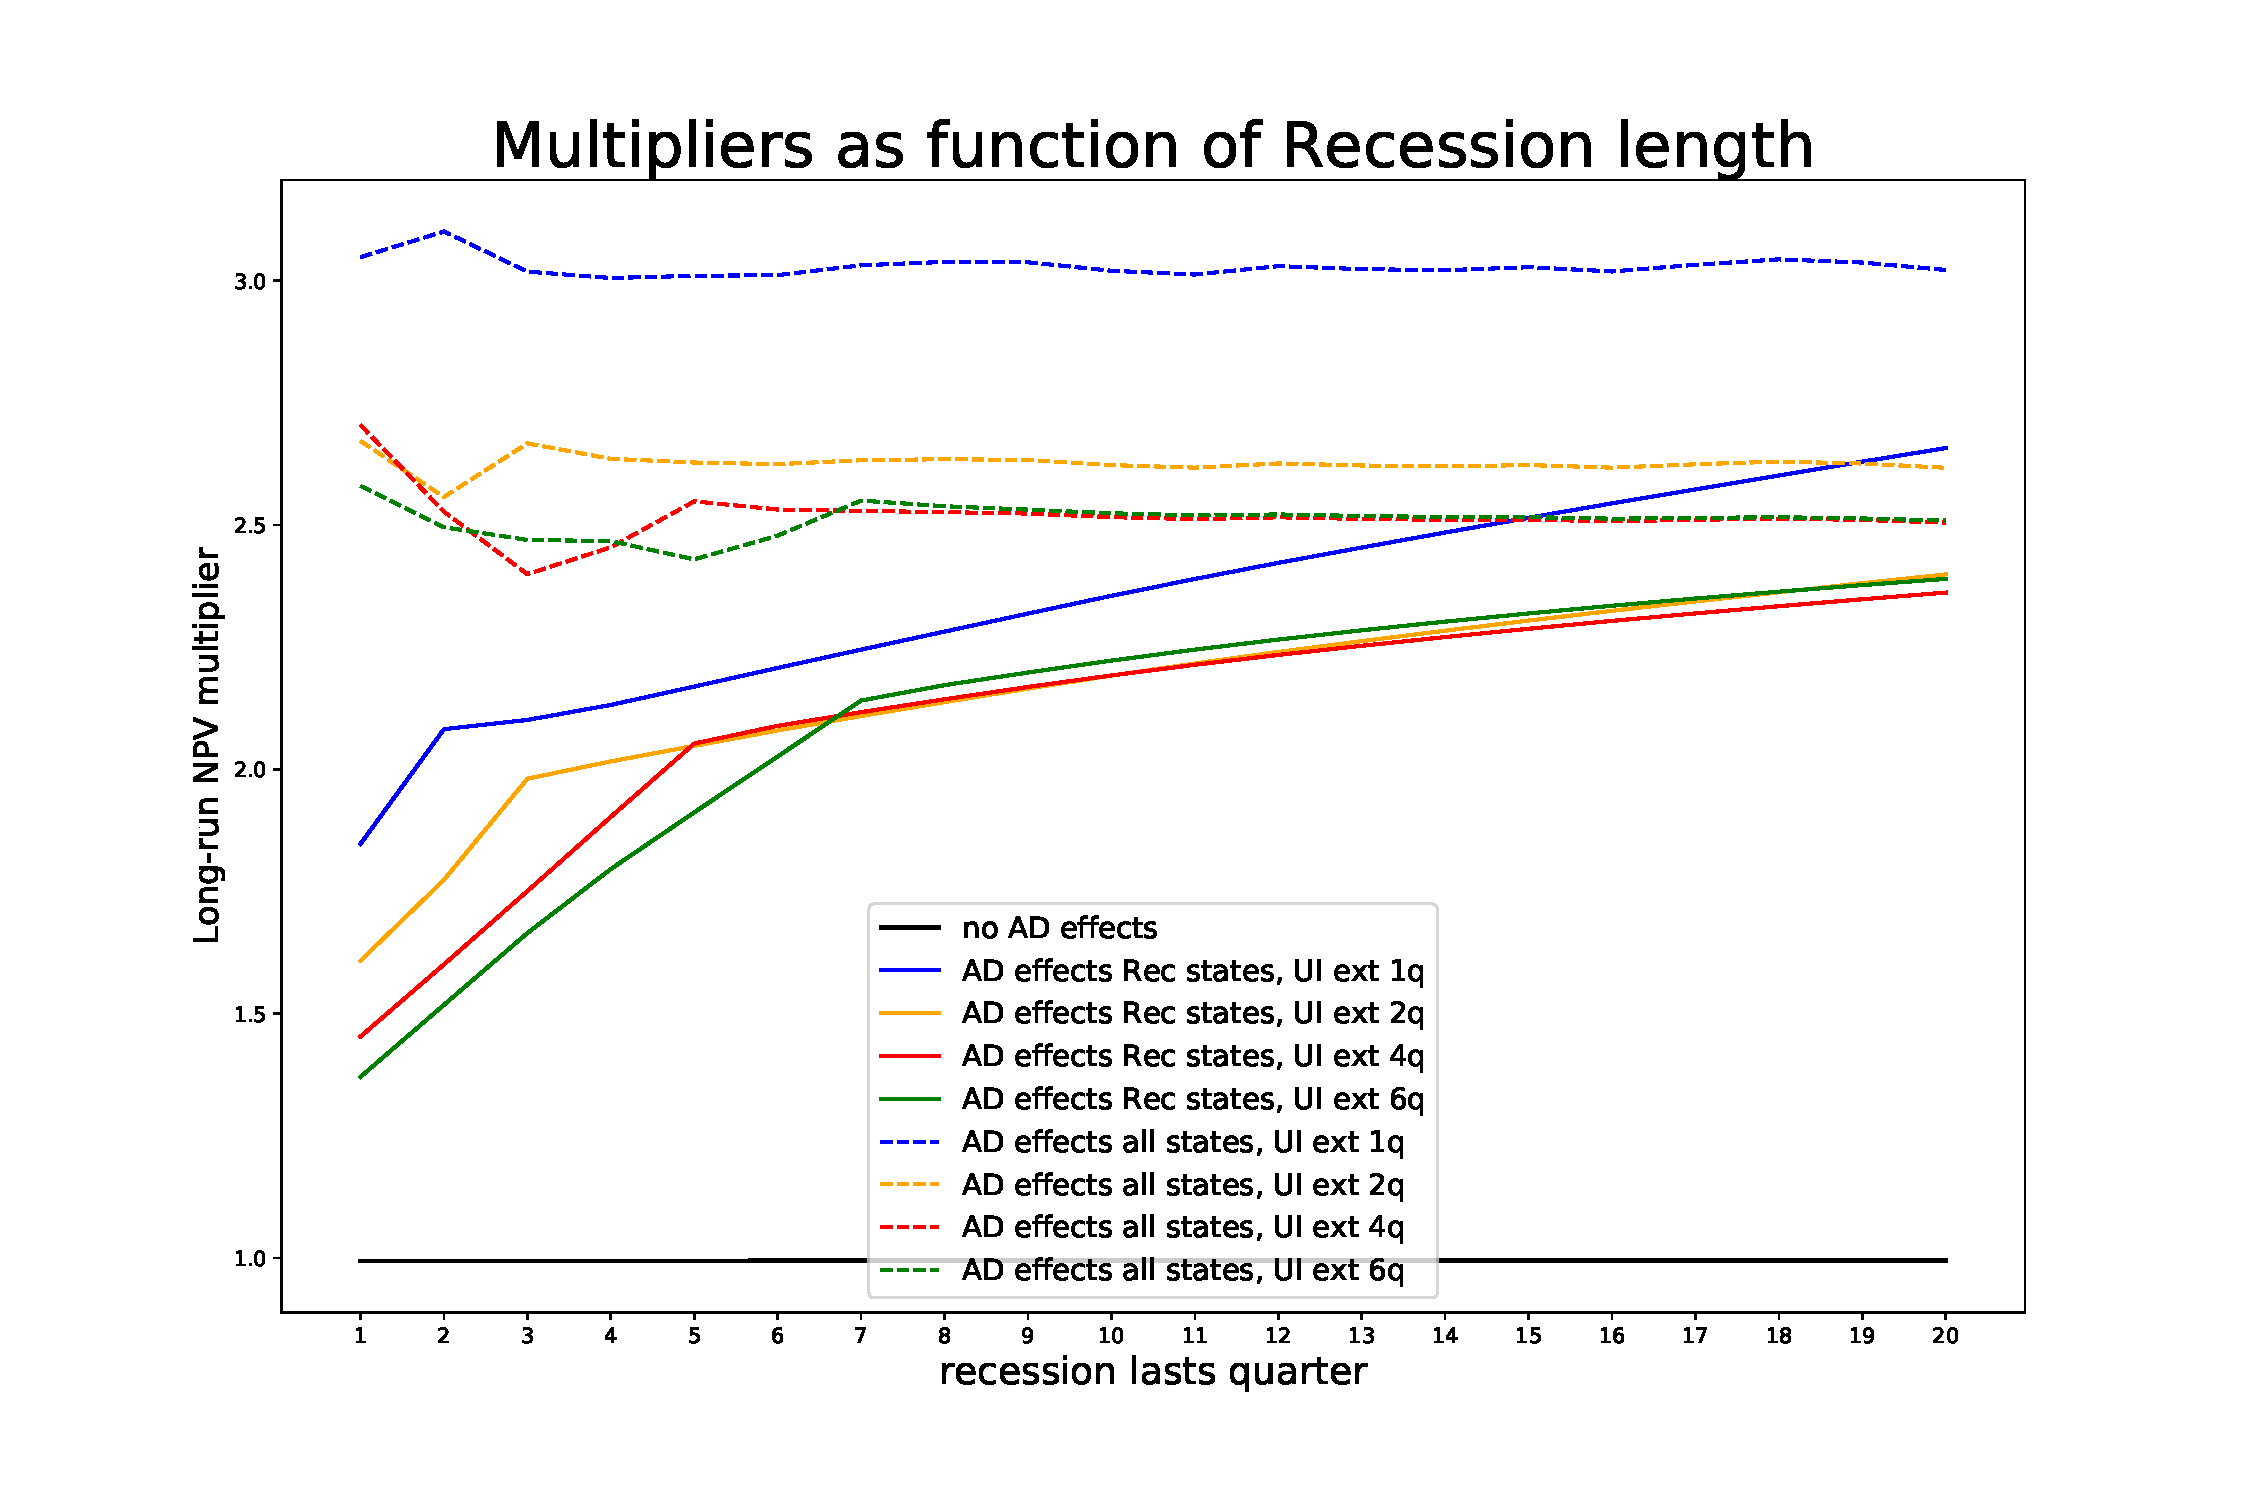
\includegraphics[width=1\linewidth]{../FullRun_Apr18_AD05_AllStates_800k/Multipliers_RecLength_PolicyLength2}
	\caption{}
	\label{fig:multipliersreclengthpolicylength2}
\end{figure}

\begin{enumerate}
	\item Wiggles from previous update disappeared with more agents (size of UI extension policy was the issue)
	\item Multipliers higher because AD effects are present in all states
	\item Length of recession does not play a role anymore
	\item after 20q small diff between all states / only rec state curves (remaing diffs probably still due to numerical error)
\end{enumerate}

	
\section{Update - Apr 7th 2021}

\subsection{Multipliers}
\begin{table}[htb]
	\centering
	\begin{tabular}{@{}llll@{}}
		\toprule
		Experiment  	& no AD effects & AD only in Rec. states 	& AD in all states \\ \midrule
		Payroll tax cut & 1 			& 1.3   			& 1.9  \\
		UI extension    & 1 			& 1.9 				& 2.2     \\ \bottomrule
	\end{tabular}	
	\caption{Long-run multipliers for each policy intervention }
	\label{tab:NPVADelas}
\end{table}

Difference to last update: UI multiplier lower (down from 5 to 1.9!). Reason was a bug that led to the UI extension being simulated under the assumption of no recession for SOME states, while the stimulus was calcuated under the assumption that the baseline was a recession.

\FloatBarrier
\subsection{Multipliers under different recession / policy lengths}
\begin{figure}[h]
	\centering
	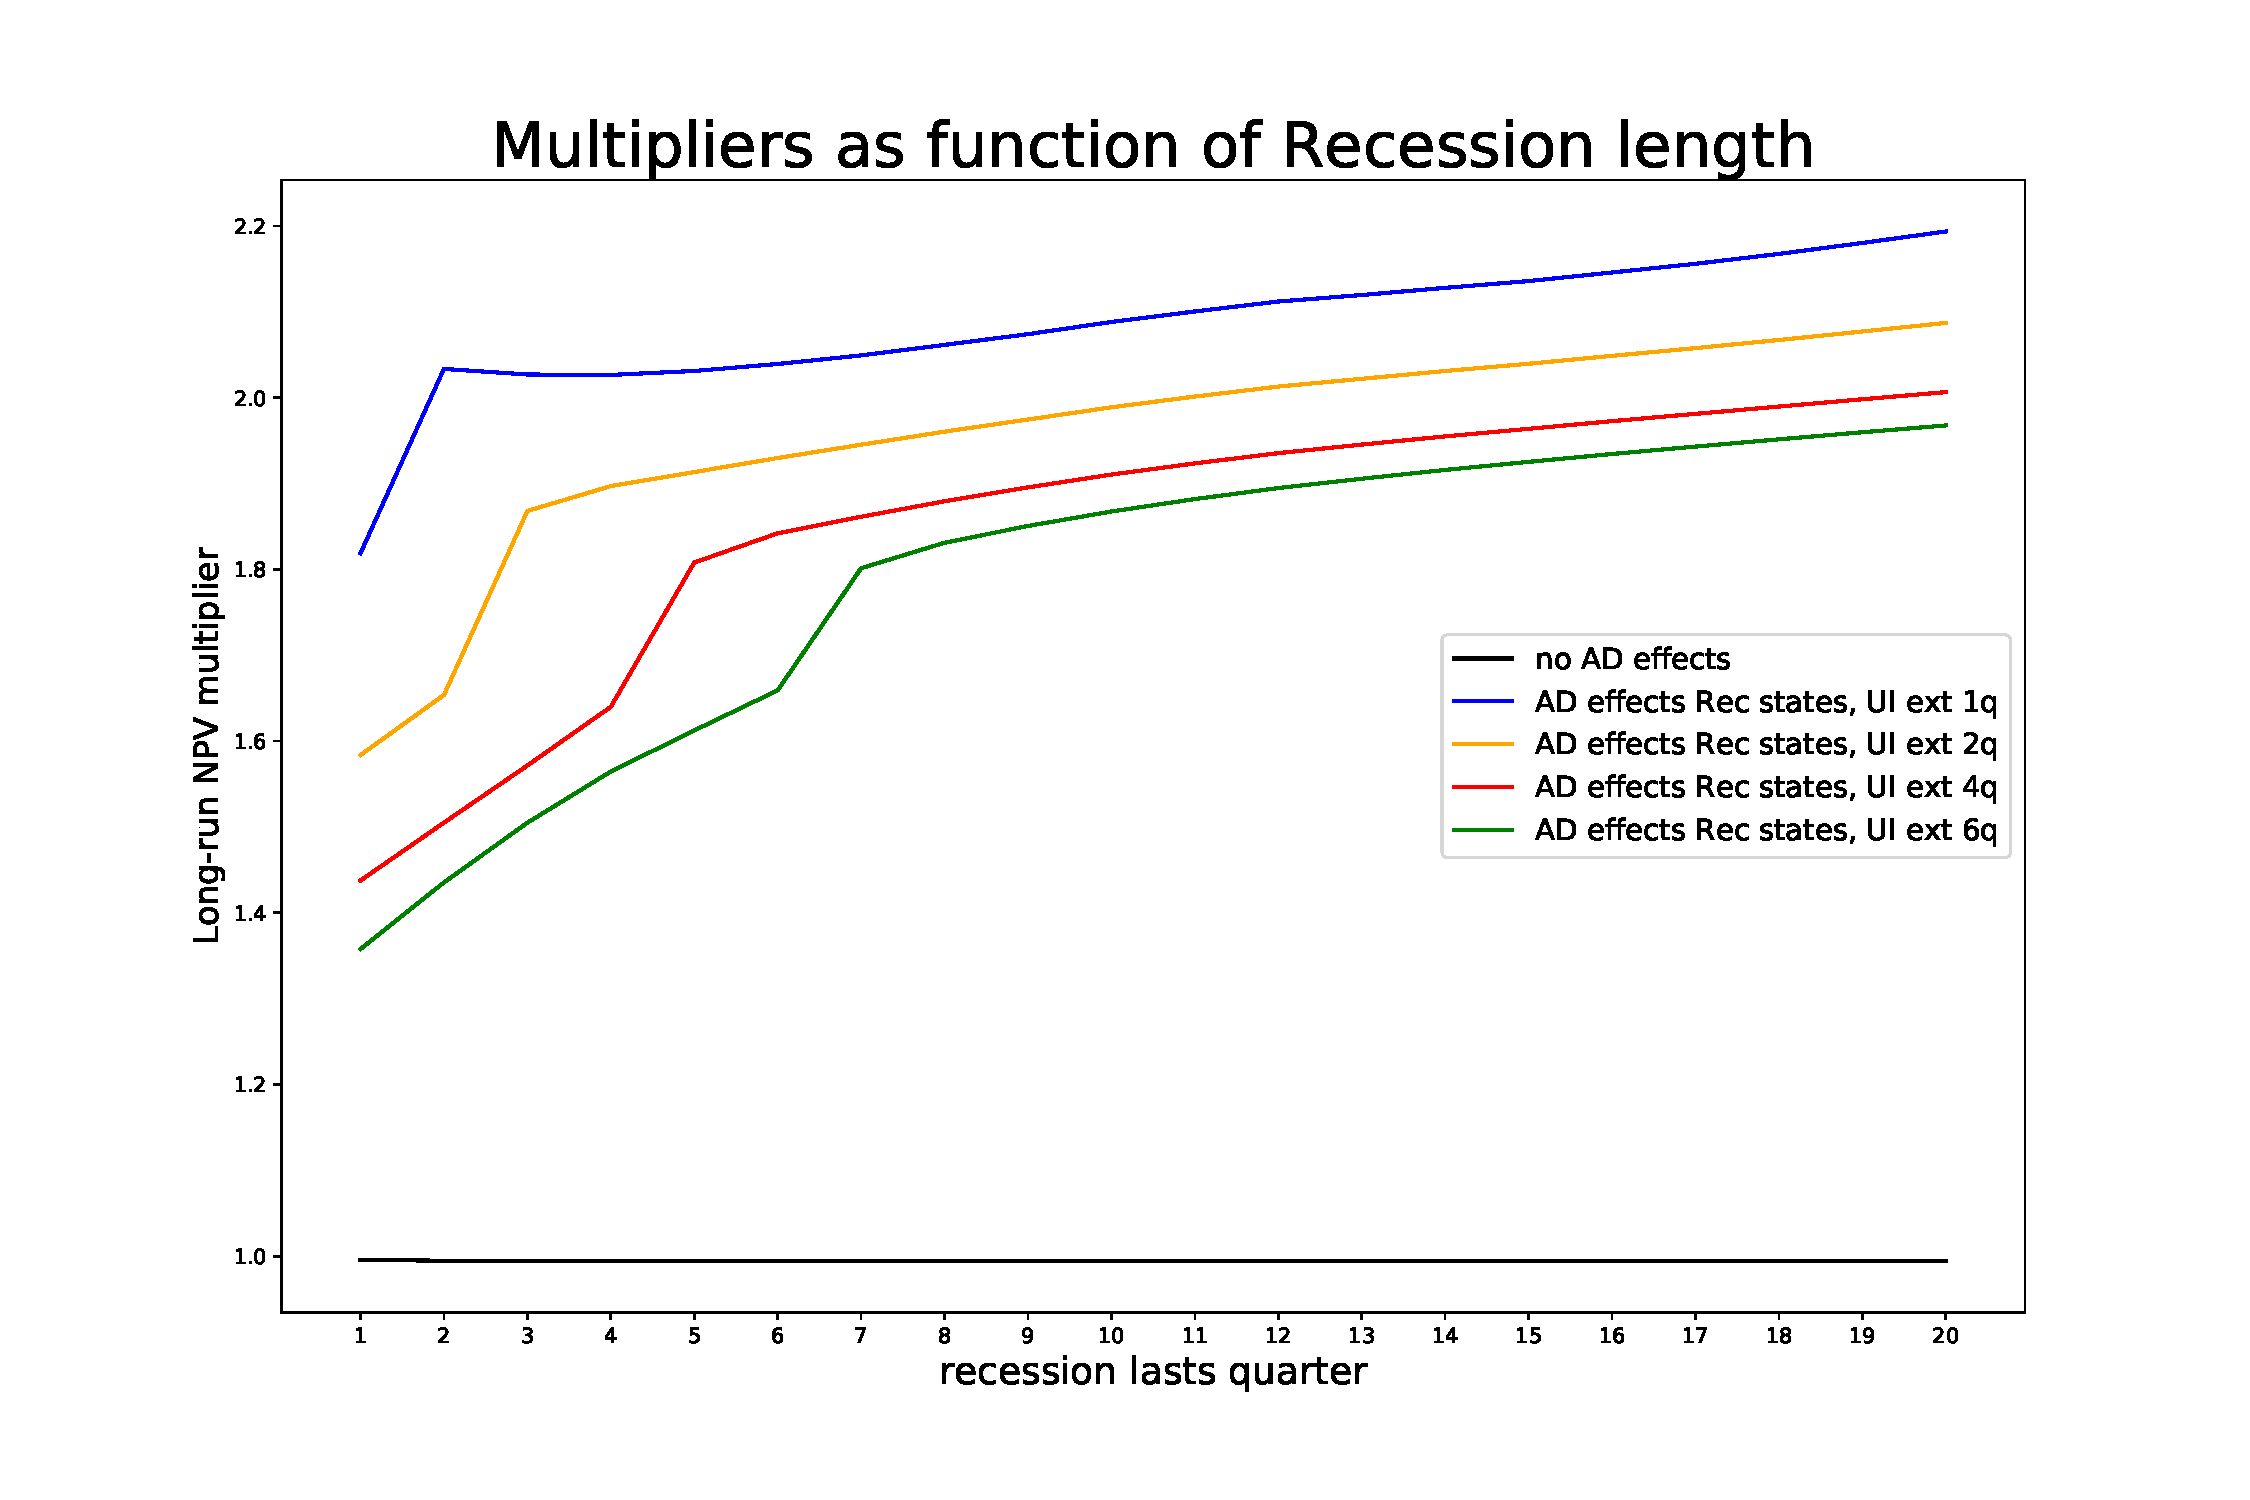
\includegraphics[width=1\linewidth]{../FullRun_Apr04_AD05_AllStates/Multipliers_RecLength_PolicyLength1}
\end{figure}

\begin{enumerate}
	\item The longer the recesssion the higher the mulitplier: Clear!
	\item For short recessions: the shorter the UI extension in length, the higher the multiplier. Reason: A higher share of the policy expenditure occur during the recession
	\item For longer recessions: Still a difference but smaller. Probably because left-over spending still occuring during the end of the recession
	\item Why do they not converge to the same level?
\end{enumerate}

\begin{figure}[h]
	\centering
	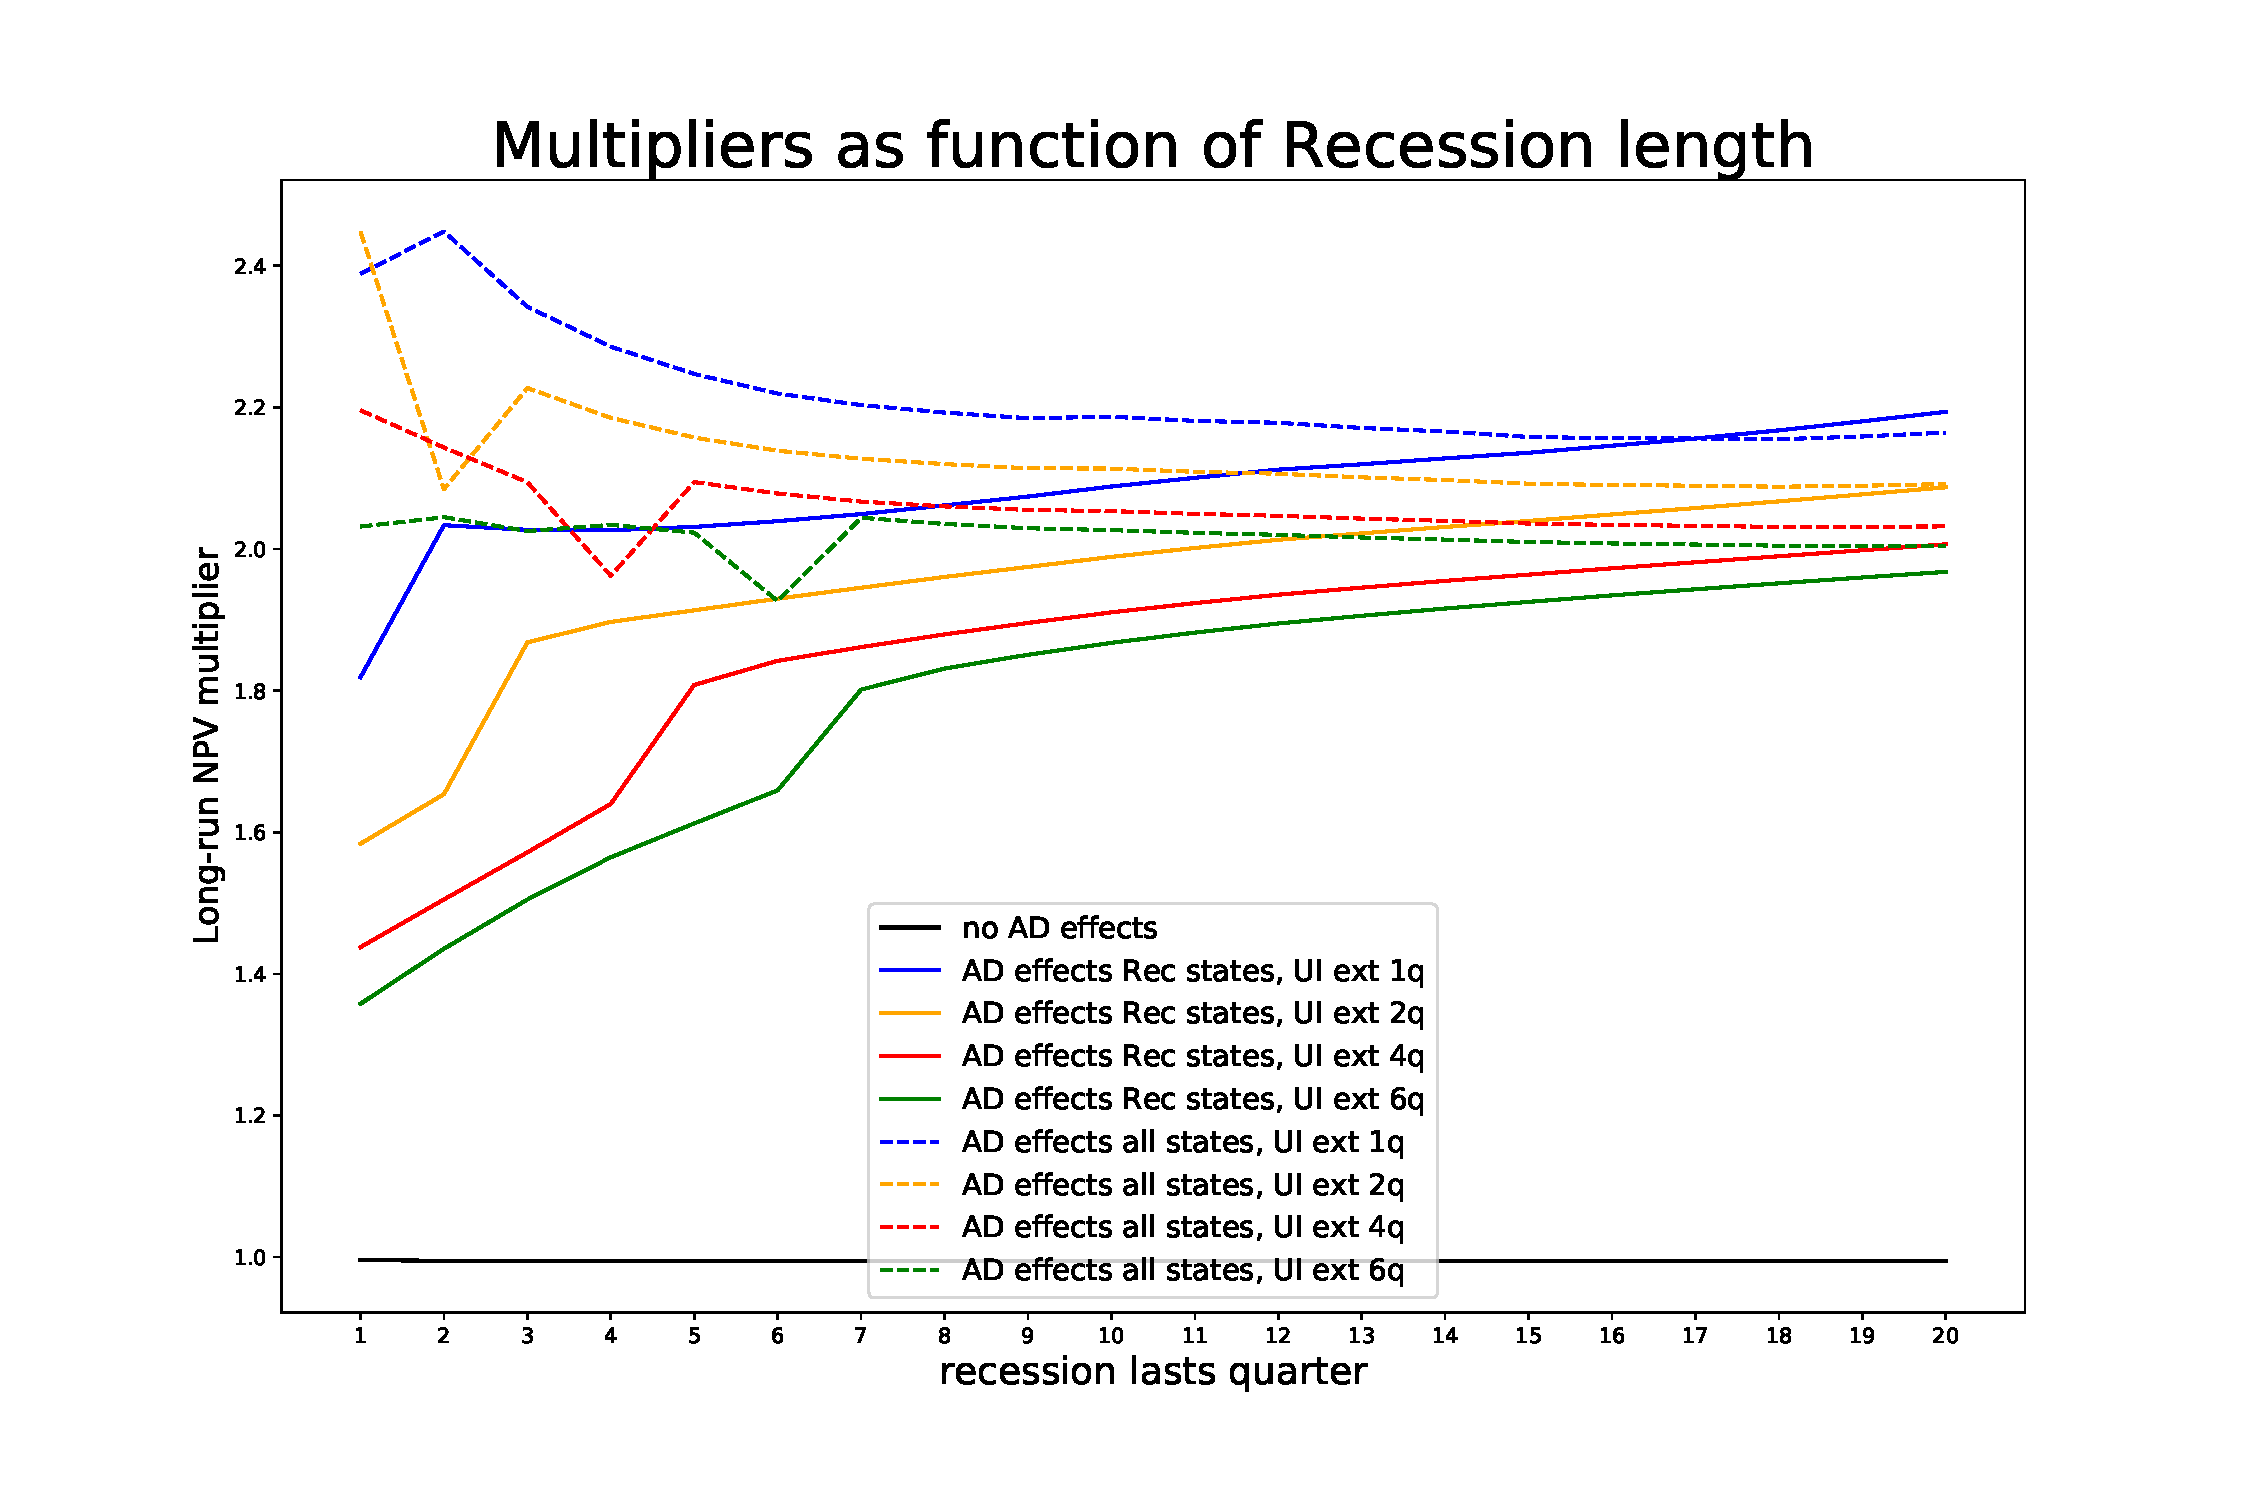
\includegraphics[width=1\linewidth]{../FullRun_Apr04_AD05_AllStates/Multipliers_RecLength_PolicyLength2}
\end{figure}

\begin{enumerate}
	\item wiggly behaviour due to a known bug, should be more or less flat
	\item The longer the recesssion the lower the multiplier. Reason: State does not matter anymore. 
	\item after 20q no diff between all states / only rec state curves
\end{enumerate}



\newpage
\FloatBarrier	
\section{Update - March 24th 2021}

\FloatBarrier
\subsection{UI extension - AD effects}



\begin{figure}[h]
	\centering
	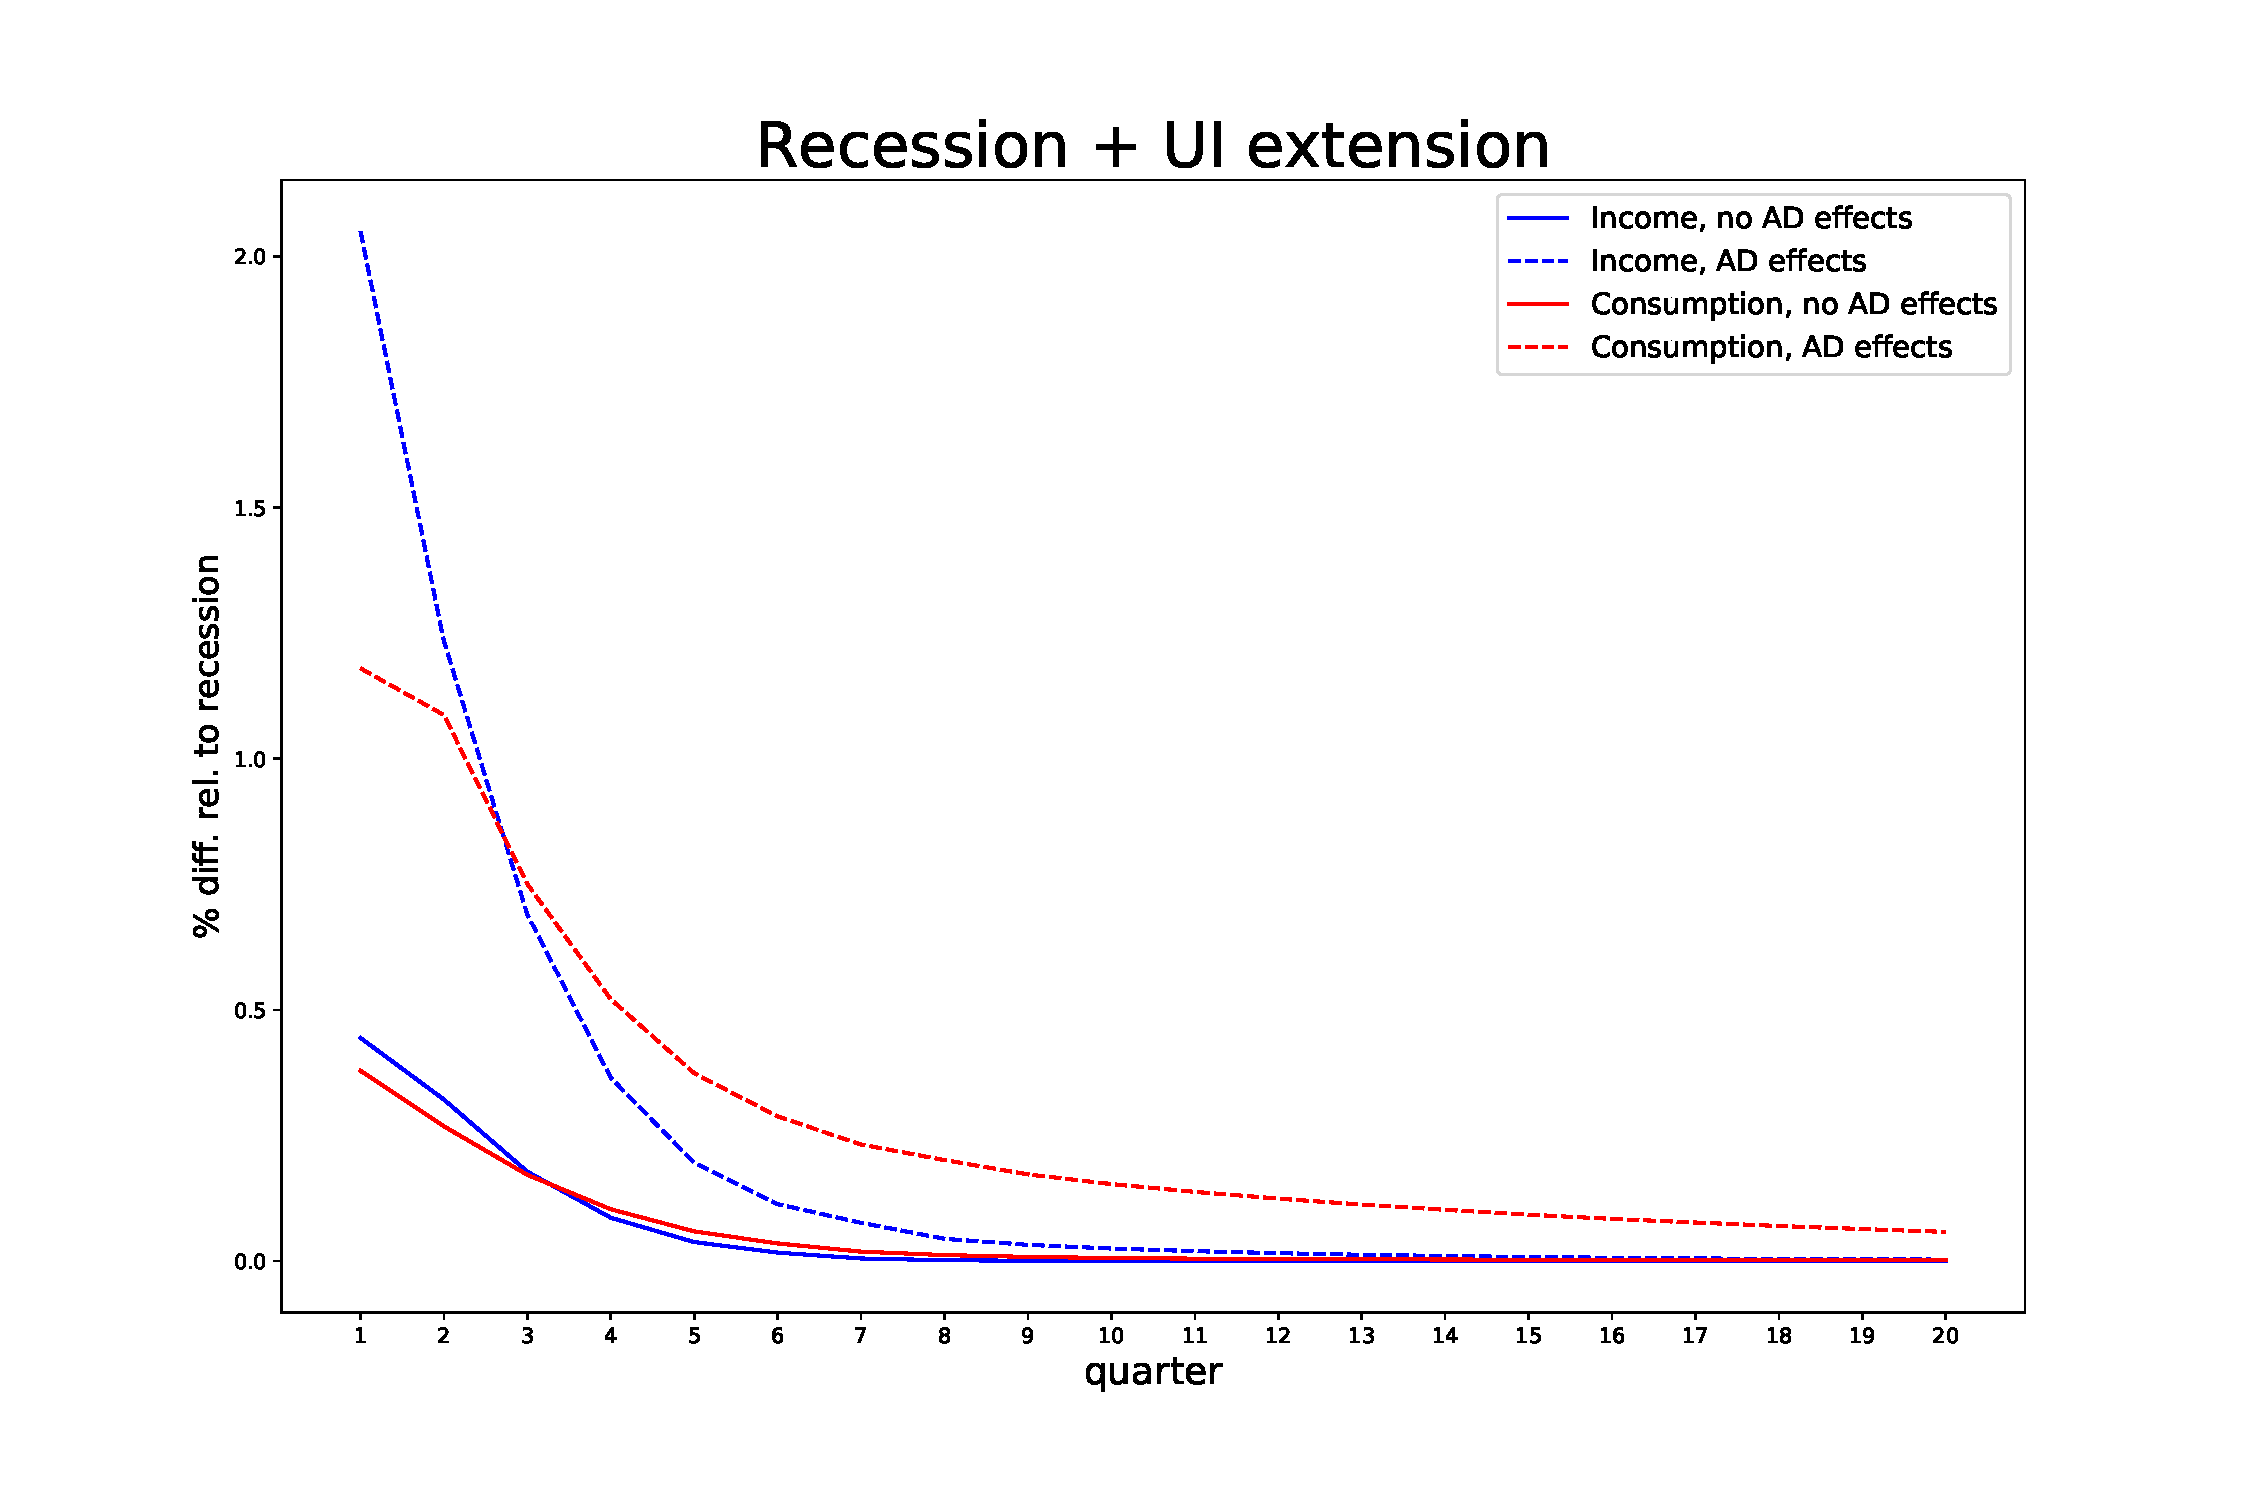
\includegraphics[width=0.7\linewidth]{../UI_AD05_new/recession_UI_relrecession}
	\caption{UI extension during recession, AD elasticity set to 0 (solid) or 0.5 (dashed)}
	\label{fig:recessionuirelrecession}
\end{figure}

\begin{figure}[h]
	\centering
	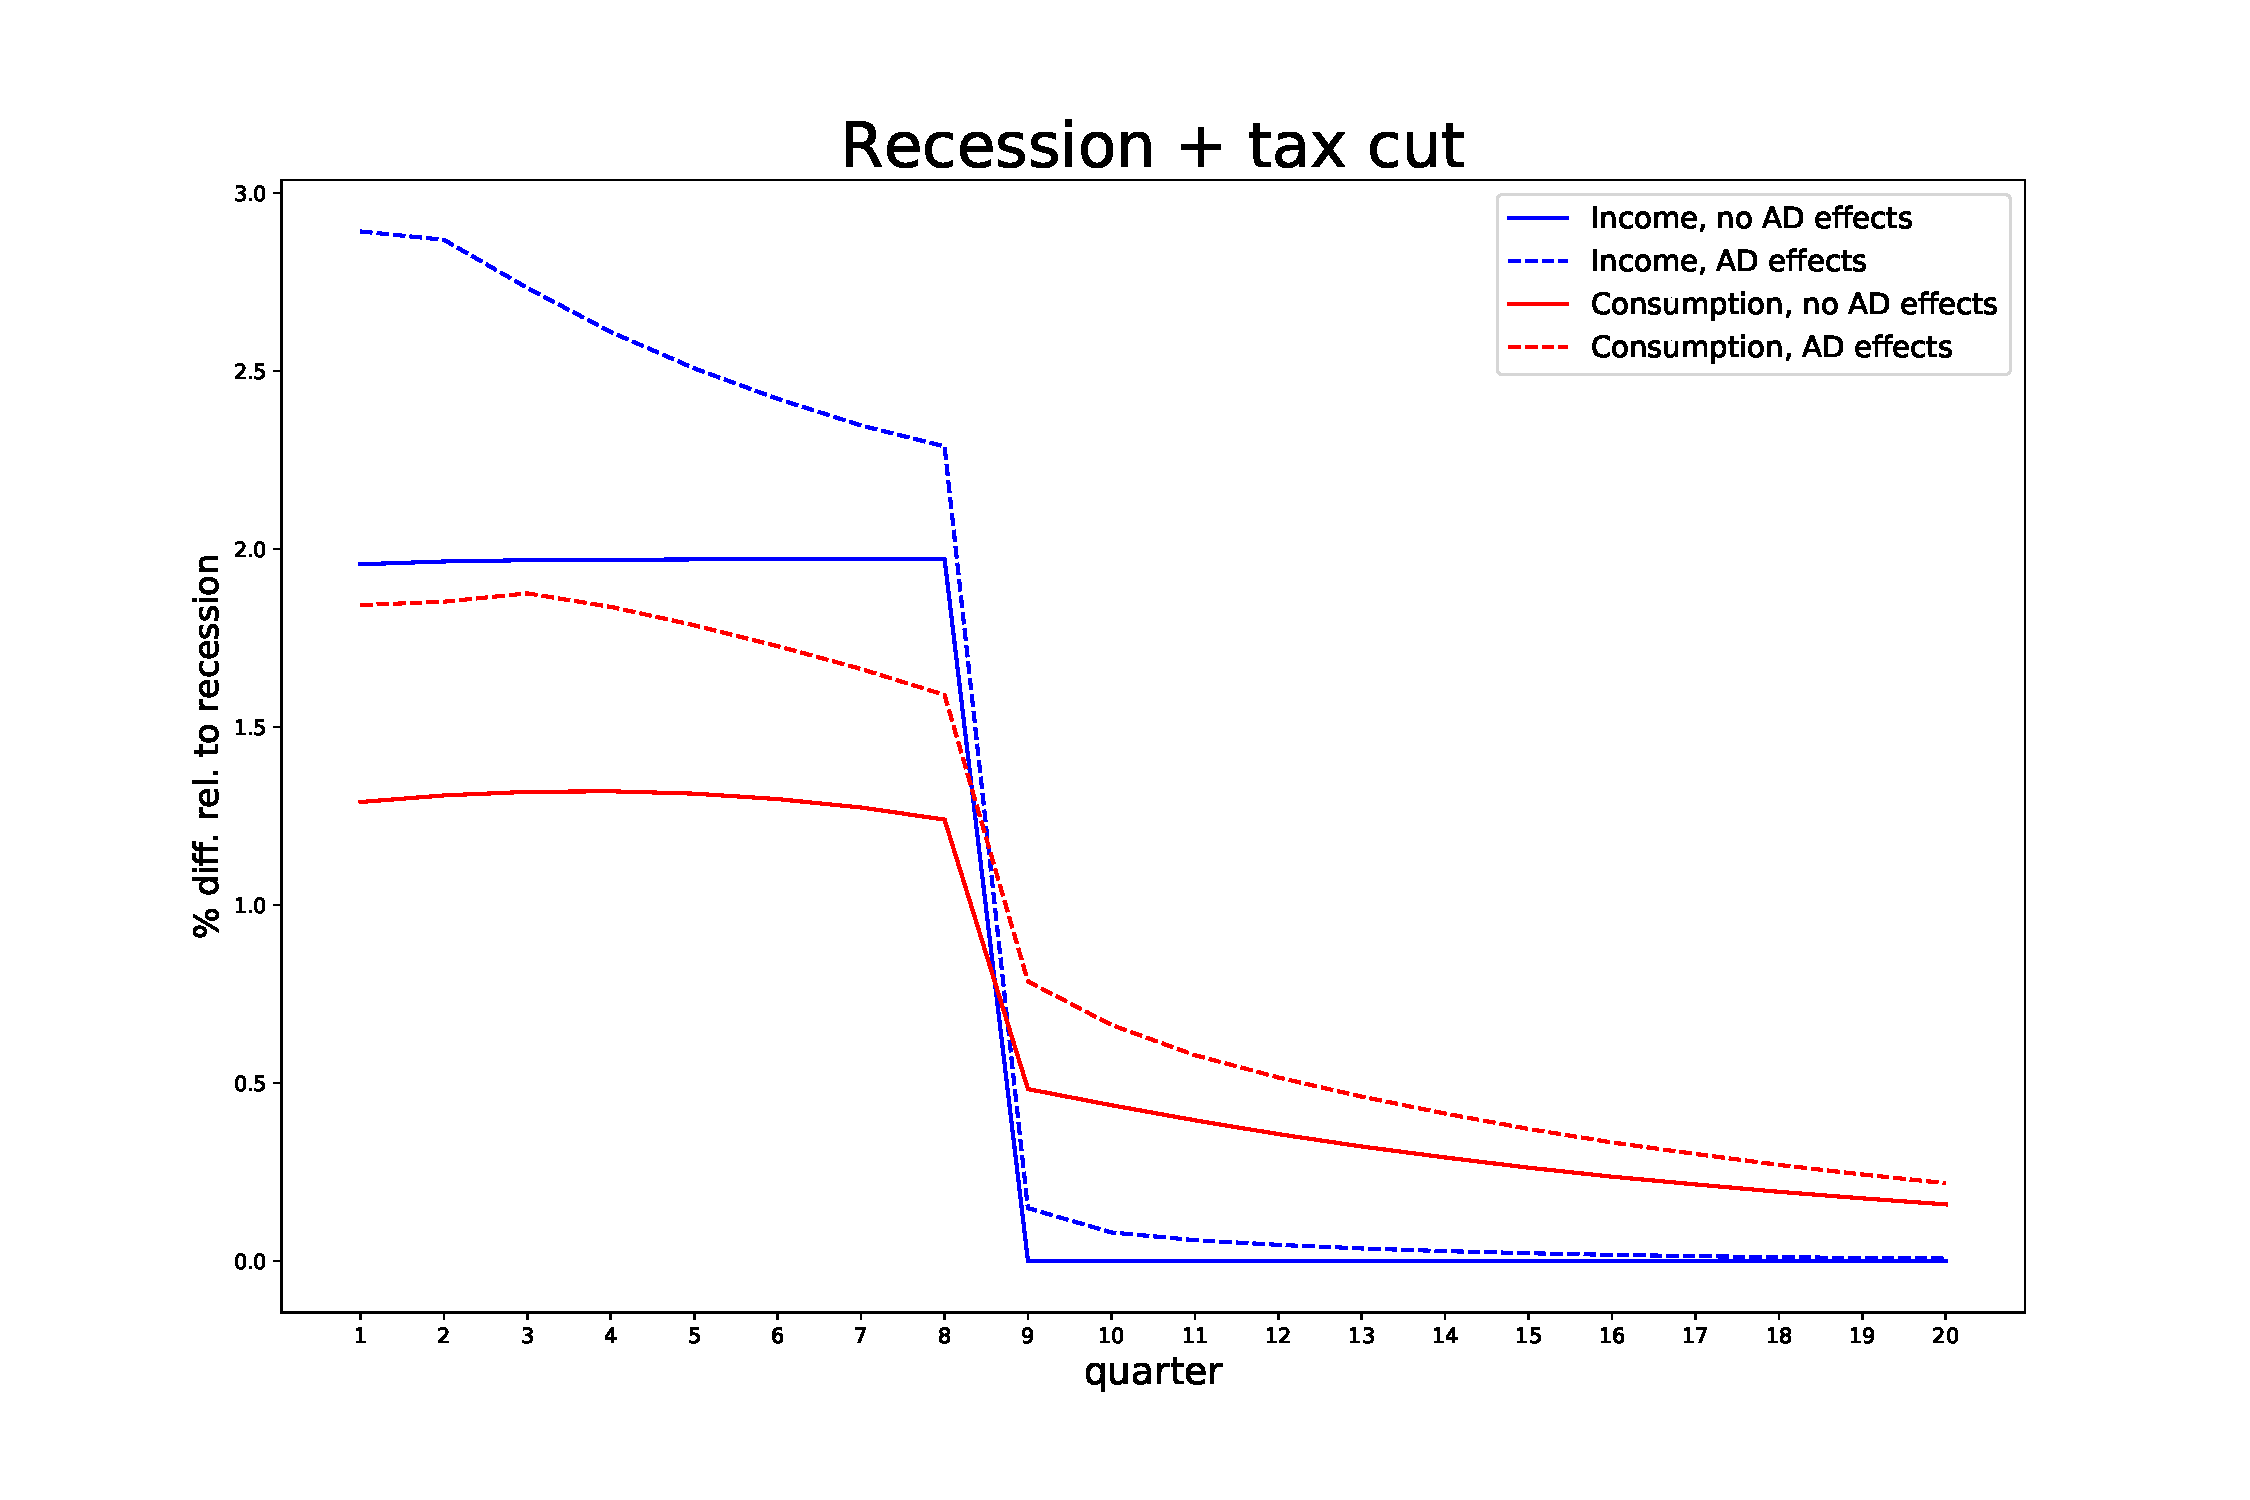
\includegraphics[width=0.7\linewidth]{../Full_Run_Mar5/recession_taxcut_relrecession}
	\caption{Payroll tax cut during recession, AD elasticity set to 0 (solid) or 0.5 (dashed)}
	\label{fig:recessiontaxcutrelrecession_statedep}
\end{figure}

\begin{figure}
	\centering
	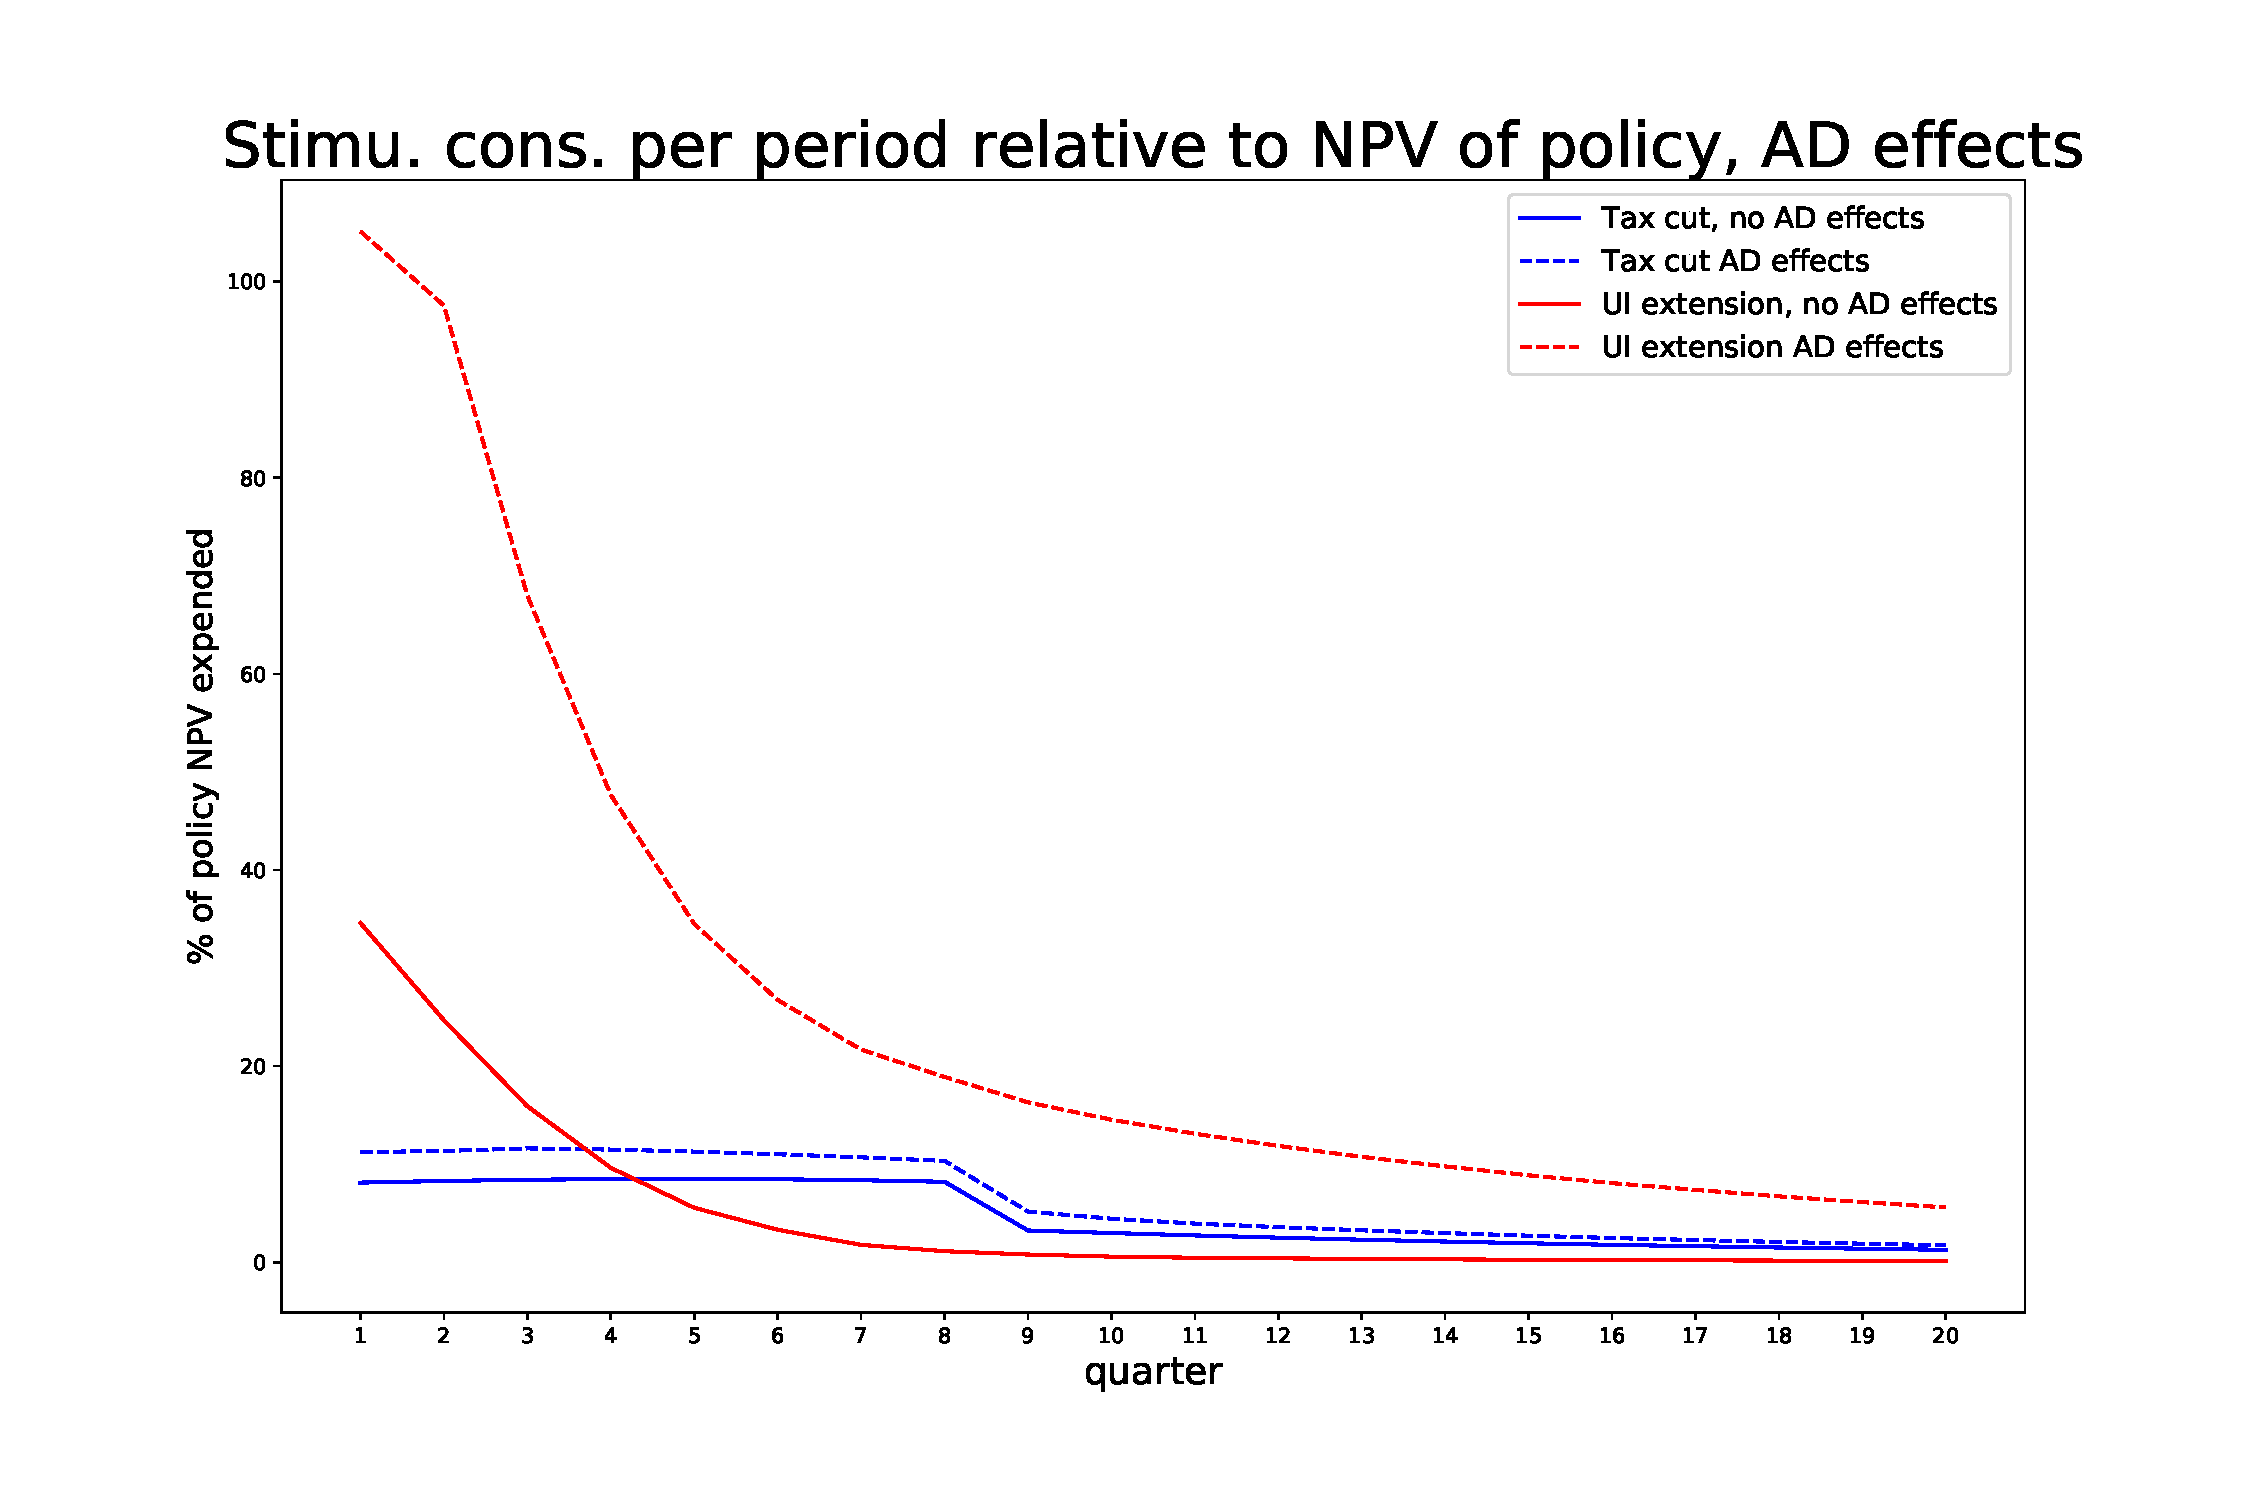
\includegraphics[width=0.7\linewidth]{../UI_AD02/Stimulus_TaxCut_AD}
	\caption{Policy experiments during recession; AD elasticity set to 0 (solid) or 0.5 (dashed)}
	\label{fig:npvmultipliernoad}
\end{figure}


\FloatBarrier
\subsection{Long-run (NPV) multipliers}

Figure \ref{fig:longrunmultipliertaxcutsenselas} shows the long-run multiplier for the payroll tax cut during a recession depending on the assumed elasticity of aggregate producitvity to demand (holding only in recession state). The multiplier for the payroll tax cut during a baseline is per construction 1 as the AD elasticity is zero in that case.

\begin{figure}[h]
	\centering
	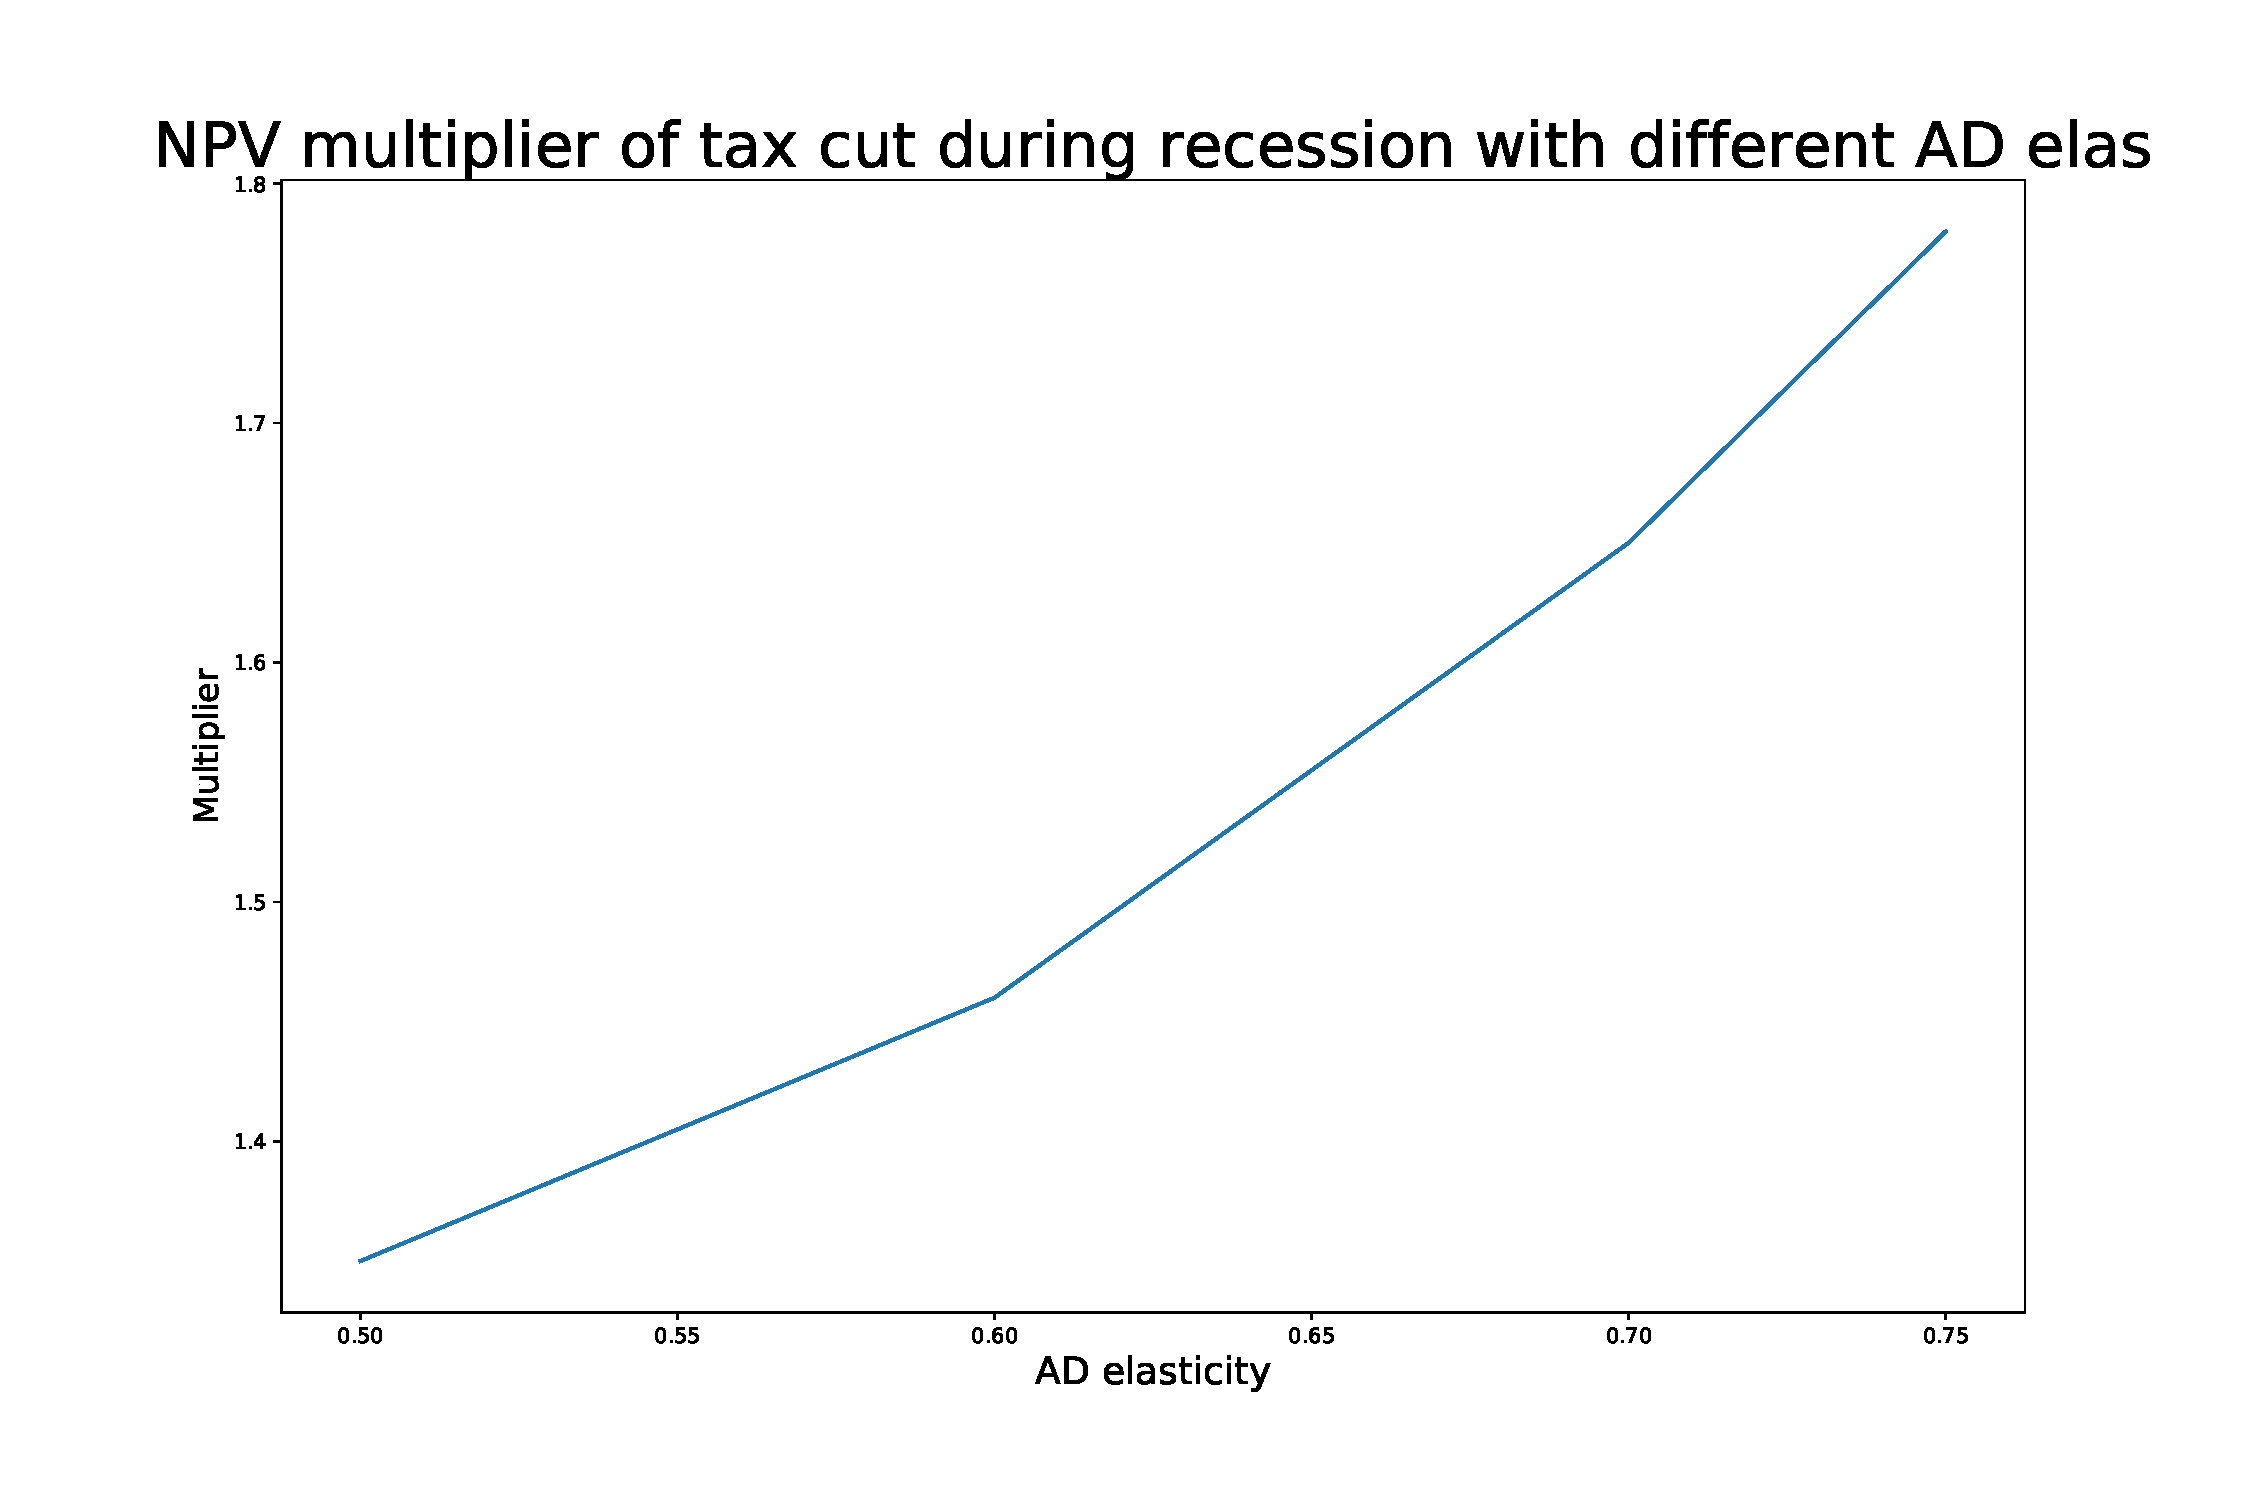
\includegraphics[width=\linewidth]{../Full_Run_Mar11_AD_Elas075/Longrun_Multiplier_TaxCut_SensElas}
	\caption{}
	\label{fig:longrunmultipliertaxcutsenselas}
\end{figure}

\begin{enumerate}
	\item Payroll tax cut gives 2 \% more income, leading to 1.3 \% more consumption (for MPC of 0.65)
	\item This leads to $(1.013)^{0.5}$ more income, hence a total increase in income by 2.65 \%, implying a 1.7 \% increase in consumption
	\item This leads to$(1.017)^{0.5}$ more income, hence a total increase in income by 2.9 \%, implying a .... \% increase in consumption
	\item and so on...
\end{enumerate}

Alternative

\begin{enumerate}
	\item Let us for arguments sake consider a 1q payroll tax cut increasing income by 1 \% and the MPC is 1
	\item Then for an AD elasticity of 1, the 1 \% higher income leads to 1 \% more consumption which leads to 1 more \% income and again 1 \% more consumption and so on forever
	\item Let now assume the MPC is only 50 \%, and the remaining 50 \% are expended in q2
	\item The likelihood that the recession is still there in q2 is 100 \%
	\item In q1: 1 \% more income -> 0.5 \% more consumption -> additional 0.5 \% income -> 0.25 \% more consumption ->
	\item In q2: 0.5 \% more consumption -> 0.5\% more income -> additional 0.25\% consumption and so on...
	\item Going through all qs gives high sum (not infinity though)
	\item However, if recession ends, sum is reduced!
	\item Also, the higher the initial MPC is the stronger will this cascade be and less important the length of recession
\end{enumerate}


Table \ref{tab:NPVADelas} shows the same information in form of a table including also the results for the Unemployment insurance extension.

\begin{table}[htb]
	\centering
	\begin{tabular}{@{}lllll@{}}
		\toprule
		Experiment \textbackslash AD-Elas & 0 & 0.2 & 0.5  & 0.75 \\ \midrule
		Payroll tax cut                   & 1 & -   & 1.35 & 1.8  \\
		UI extension                      & 1 & 2.4 & 5.6  & -    \\ \bottomrule
	\end{tabular}	
	\caption{Long-run multipliers for each policy intervention for different AD elasticities}
	\label{tab:NPVADelas}
\end{table}

\begin{enumerate}
	\item UI extension gives 0.5 \% more income (10 \% unepmloyed x 0.25 (additional replacement rate) x 20 \% in need of extension), leading to 0.5 \% more consumption (for MPC of 1 by unemployed)
	\item This leads to $(1.005)^{0.5}$ more income, i.e. 0.25 \% more income in the aggregate and continuing cascade
	\item However larger share of spending expended during recession!
\end{enumerate}


\FloatBarrier
\section{Update - March 10th 2021}	

\FloatBarrier
\subsection{Open question}

\begin{itemize}
	\item Absent AD effects, the NPV of fiscal policy intervention can be measured as: NPV of aggregate income in policy experiment - NPV of aggregate income without policy experiment
	\item But what about with AD effects?
	\item Cannot do the sasme calculation: NPV of aggregate income in policy experiment - NPV of aggregate income without policy experiment: The difference captures both policy expenditure as well as higher productivity
	\item Can we use the policy expenditure as calculated under no AD effects?
\end{itemize}

\FloatBarrier
\subsection{State-dependent AD elasticity}

\begin{itemize}
	\item Figure \ref{fig:recessiontaxcutrelrecession_statedep} shows additional income and consumption for tax cut during recession relative to recession with no tax cut, both when AD effects are present and when they are not
	\item AD effects, however, are state-dependent. Only in a recession we have an AD elasticity of 0.5
	\item Figure \ref{fig:taxcutrecdecomprelrecession} shows a decomposition. Full results are the weighted (by recession length probality) sum of different simulations with increasing length of recession. If recession stops after few quarters, then AD elasticity jumps back to zero, such that the tax cut becomes less effective. As we progress in time, the likelihood that recession has ended becomes larger, such that that gets a larger weight in the weighted sum. Over time the weighted average AD effect drops.
	\item Problably some numerical issue with q1. Income drops more going from q1 to 2 in No Tax Cut recession.
\end{itemize}

\begin{figure}
	\centering
	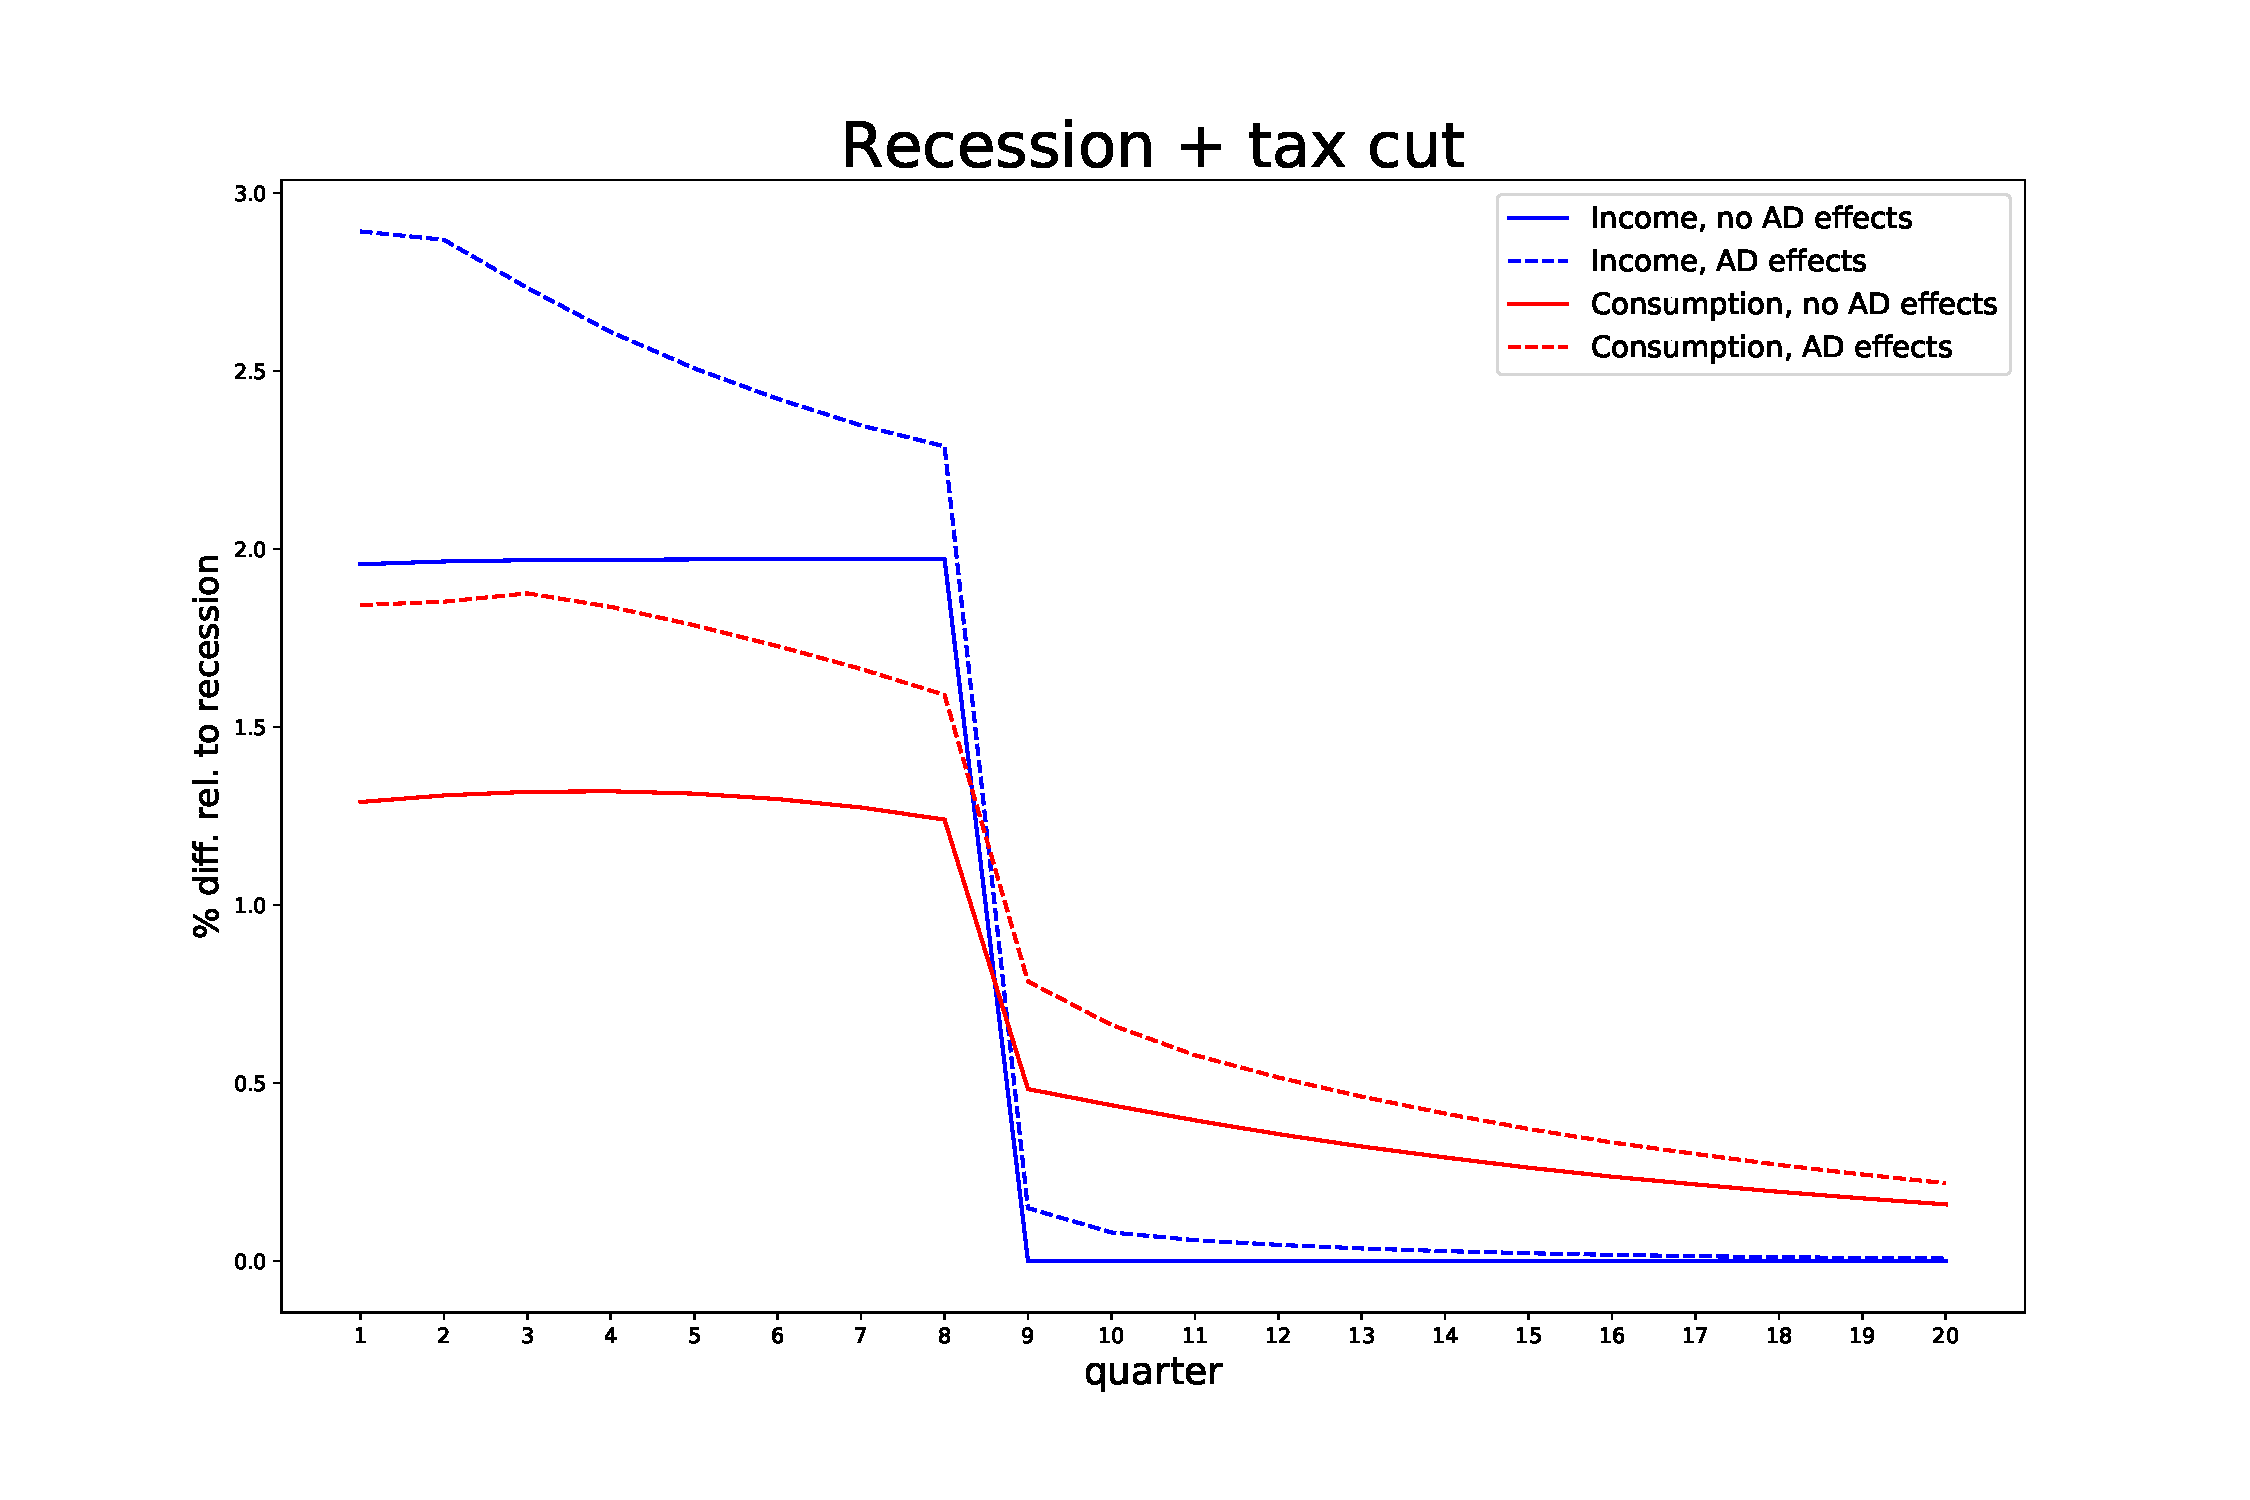
\includegraphics[width=\linewidth]{../Full_Run_Mar5/recession_taxcut_relrecession}
	\caption{}
	\label{fig:recessiontaxcutrelrecession_statedep}
\end{figure}

\begin{figure}
	\centering
	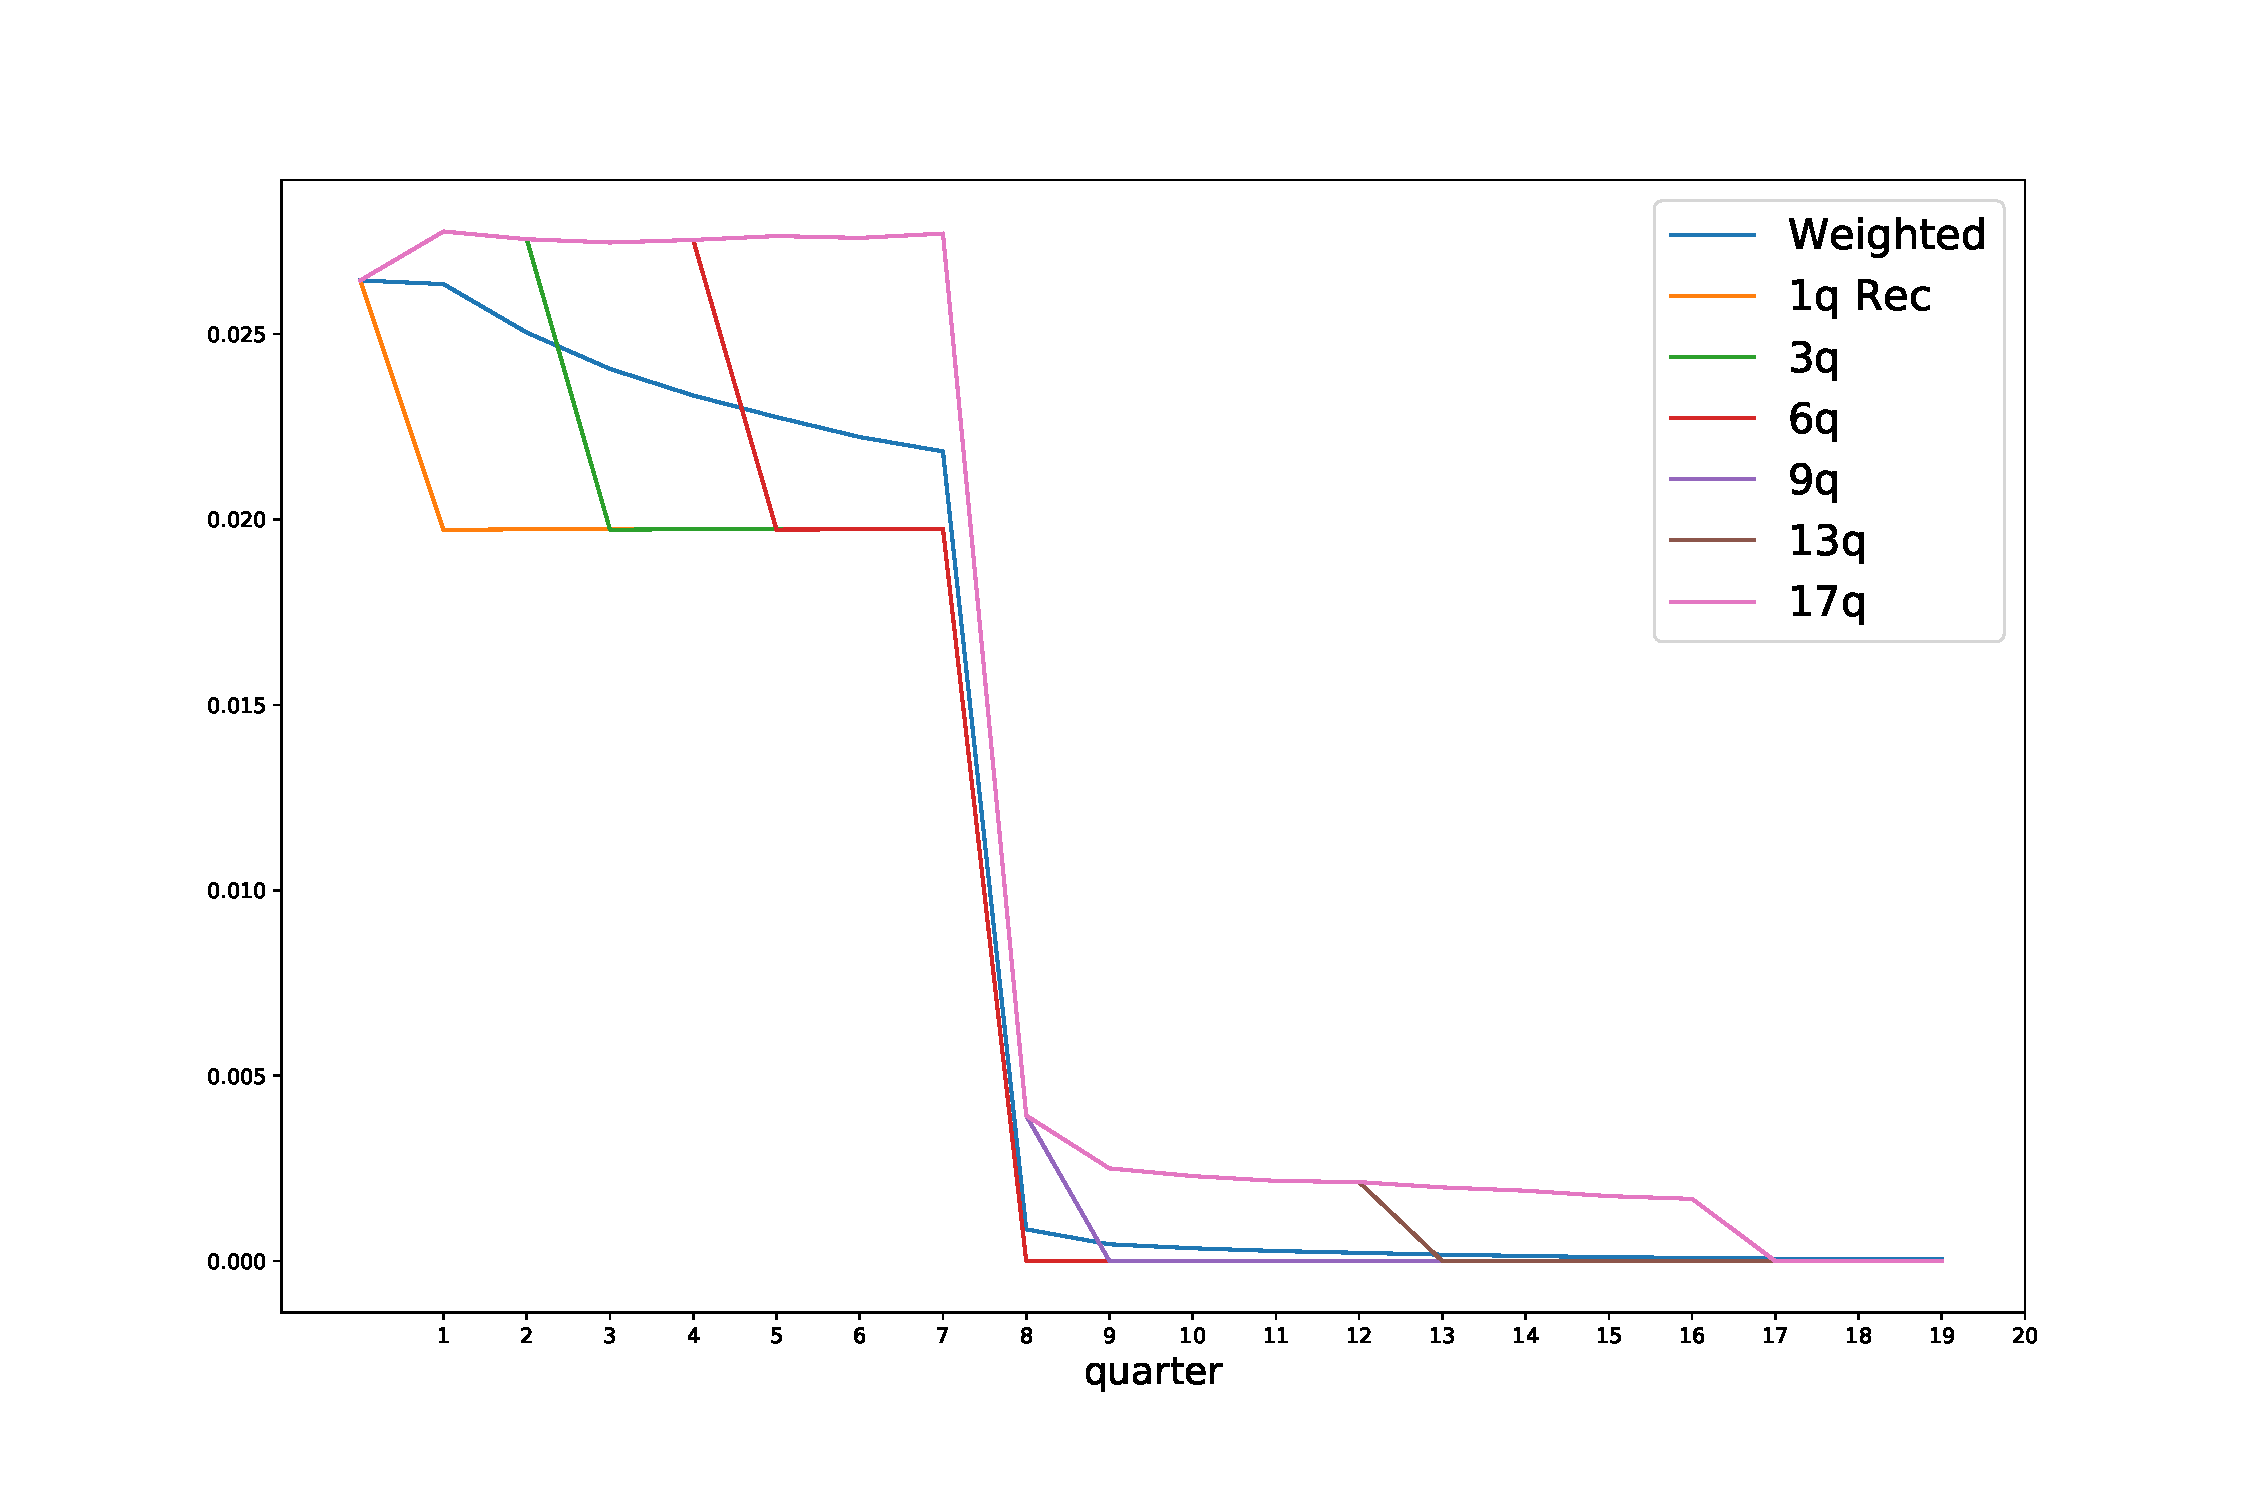
\includegraphics[width=\linewidth]{../Full_Run_Mar5/Tax_Cut_Rec_Decomp_Rel_Recession}
	\caption{}
	\label{fig:taxcutrecdecomprelrecession}
\end{figure}

\begin{figure}
	\centering
	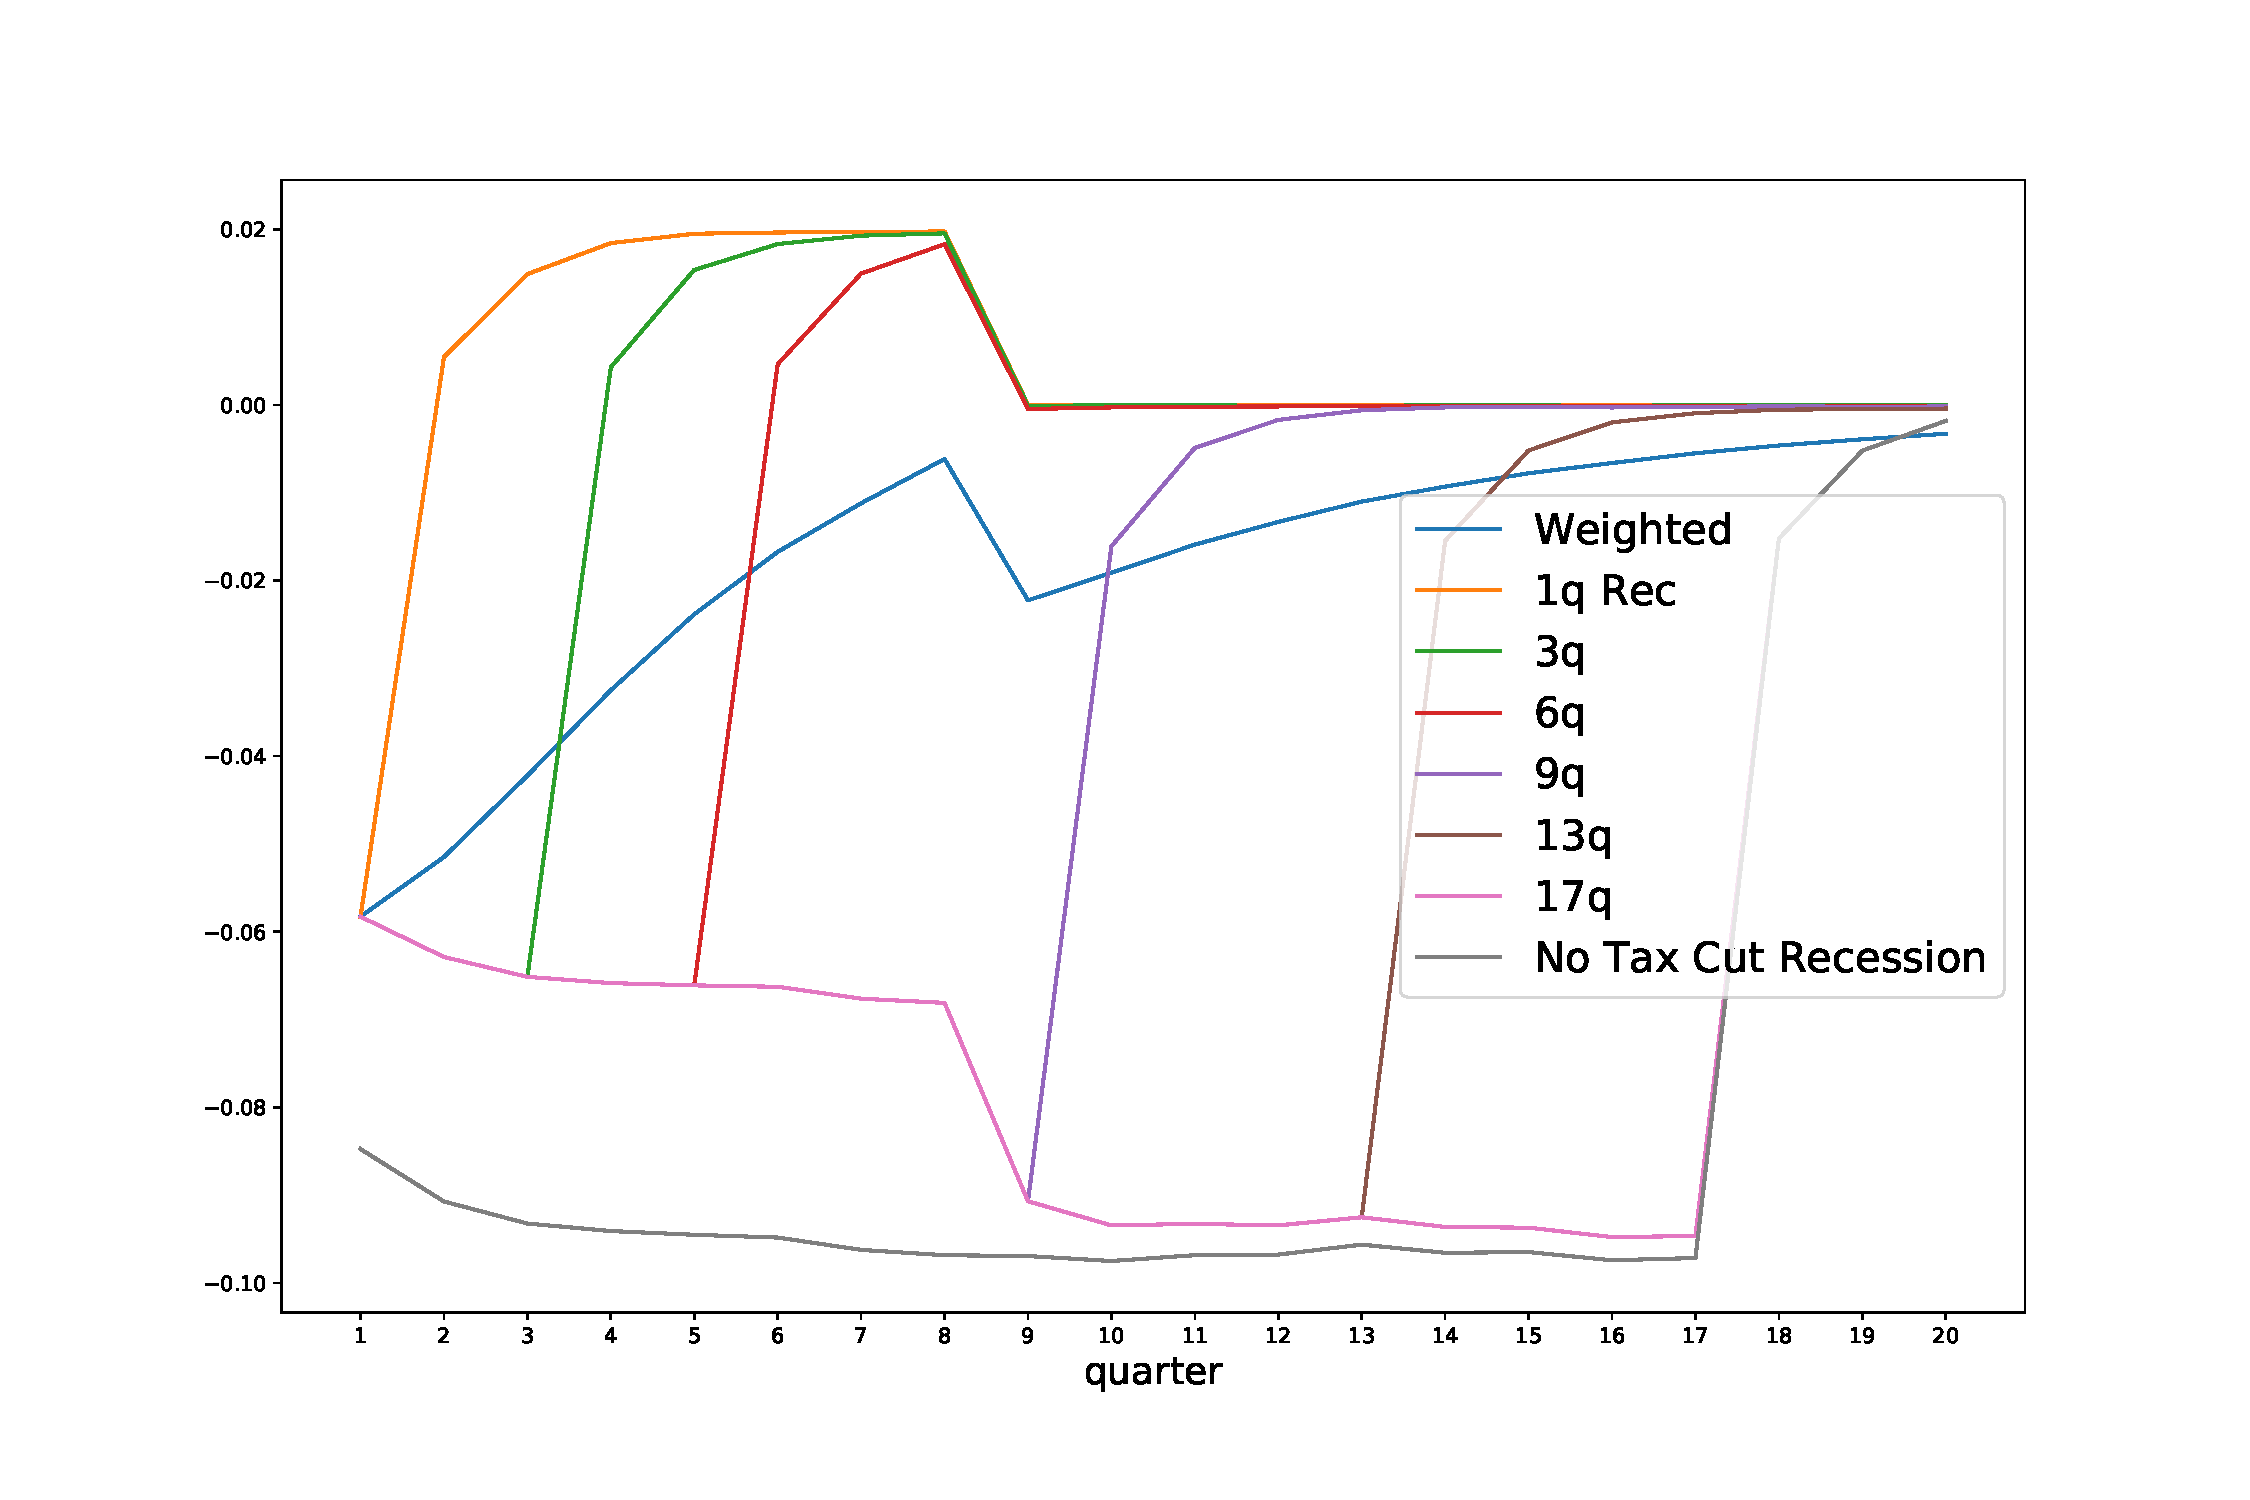
\includegraphics[width=\linewidth]{../Full_Run_Mar5/Tax_Cut_Rec_Decomp_Rel_Baseline}
	\caption{}
	\label{fig:taxcutrecdecomprelbaseline}
\end{figure}


\FloatBarrier	
\section{Update - February 24th 2021}	
\FloatBarrier
\subsection{Multipliers}

\begin{itemize}
	\item Figure \ref{fig:npvmultipliernoad} and \ref{fig:periodmultipliernoad} show different ways to plot spending / tax multipliers.
	\item The first figure shows the additional consumption created by the specific policy relative to the NPV of the total policy intervention. For example, about 35 \% of the total NPV of the UI exentension is spend by households in the very first quarter. (The value is higher is higher outside of the recession because there is less need for precautionary saving.)
	\item The secon plot shows the perid by period multiplier. The value for q1 represents the impact multiplier. Hence, about 70 \% of the additional income generated by the payroll tax cut is expended in each period, while 85 \% of the additional unemployment benefits is spent.
\end{itemize}

\begin{figure}
	\centering
	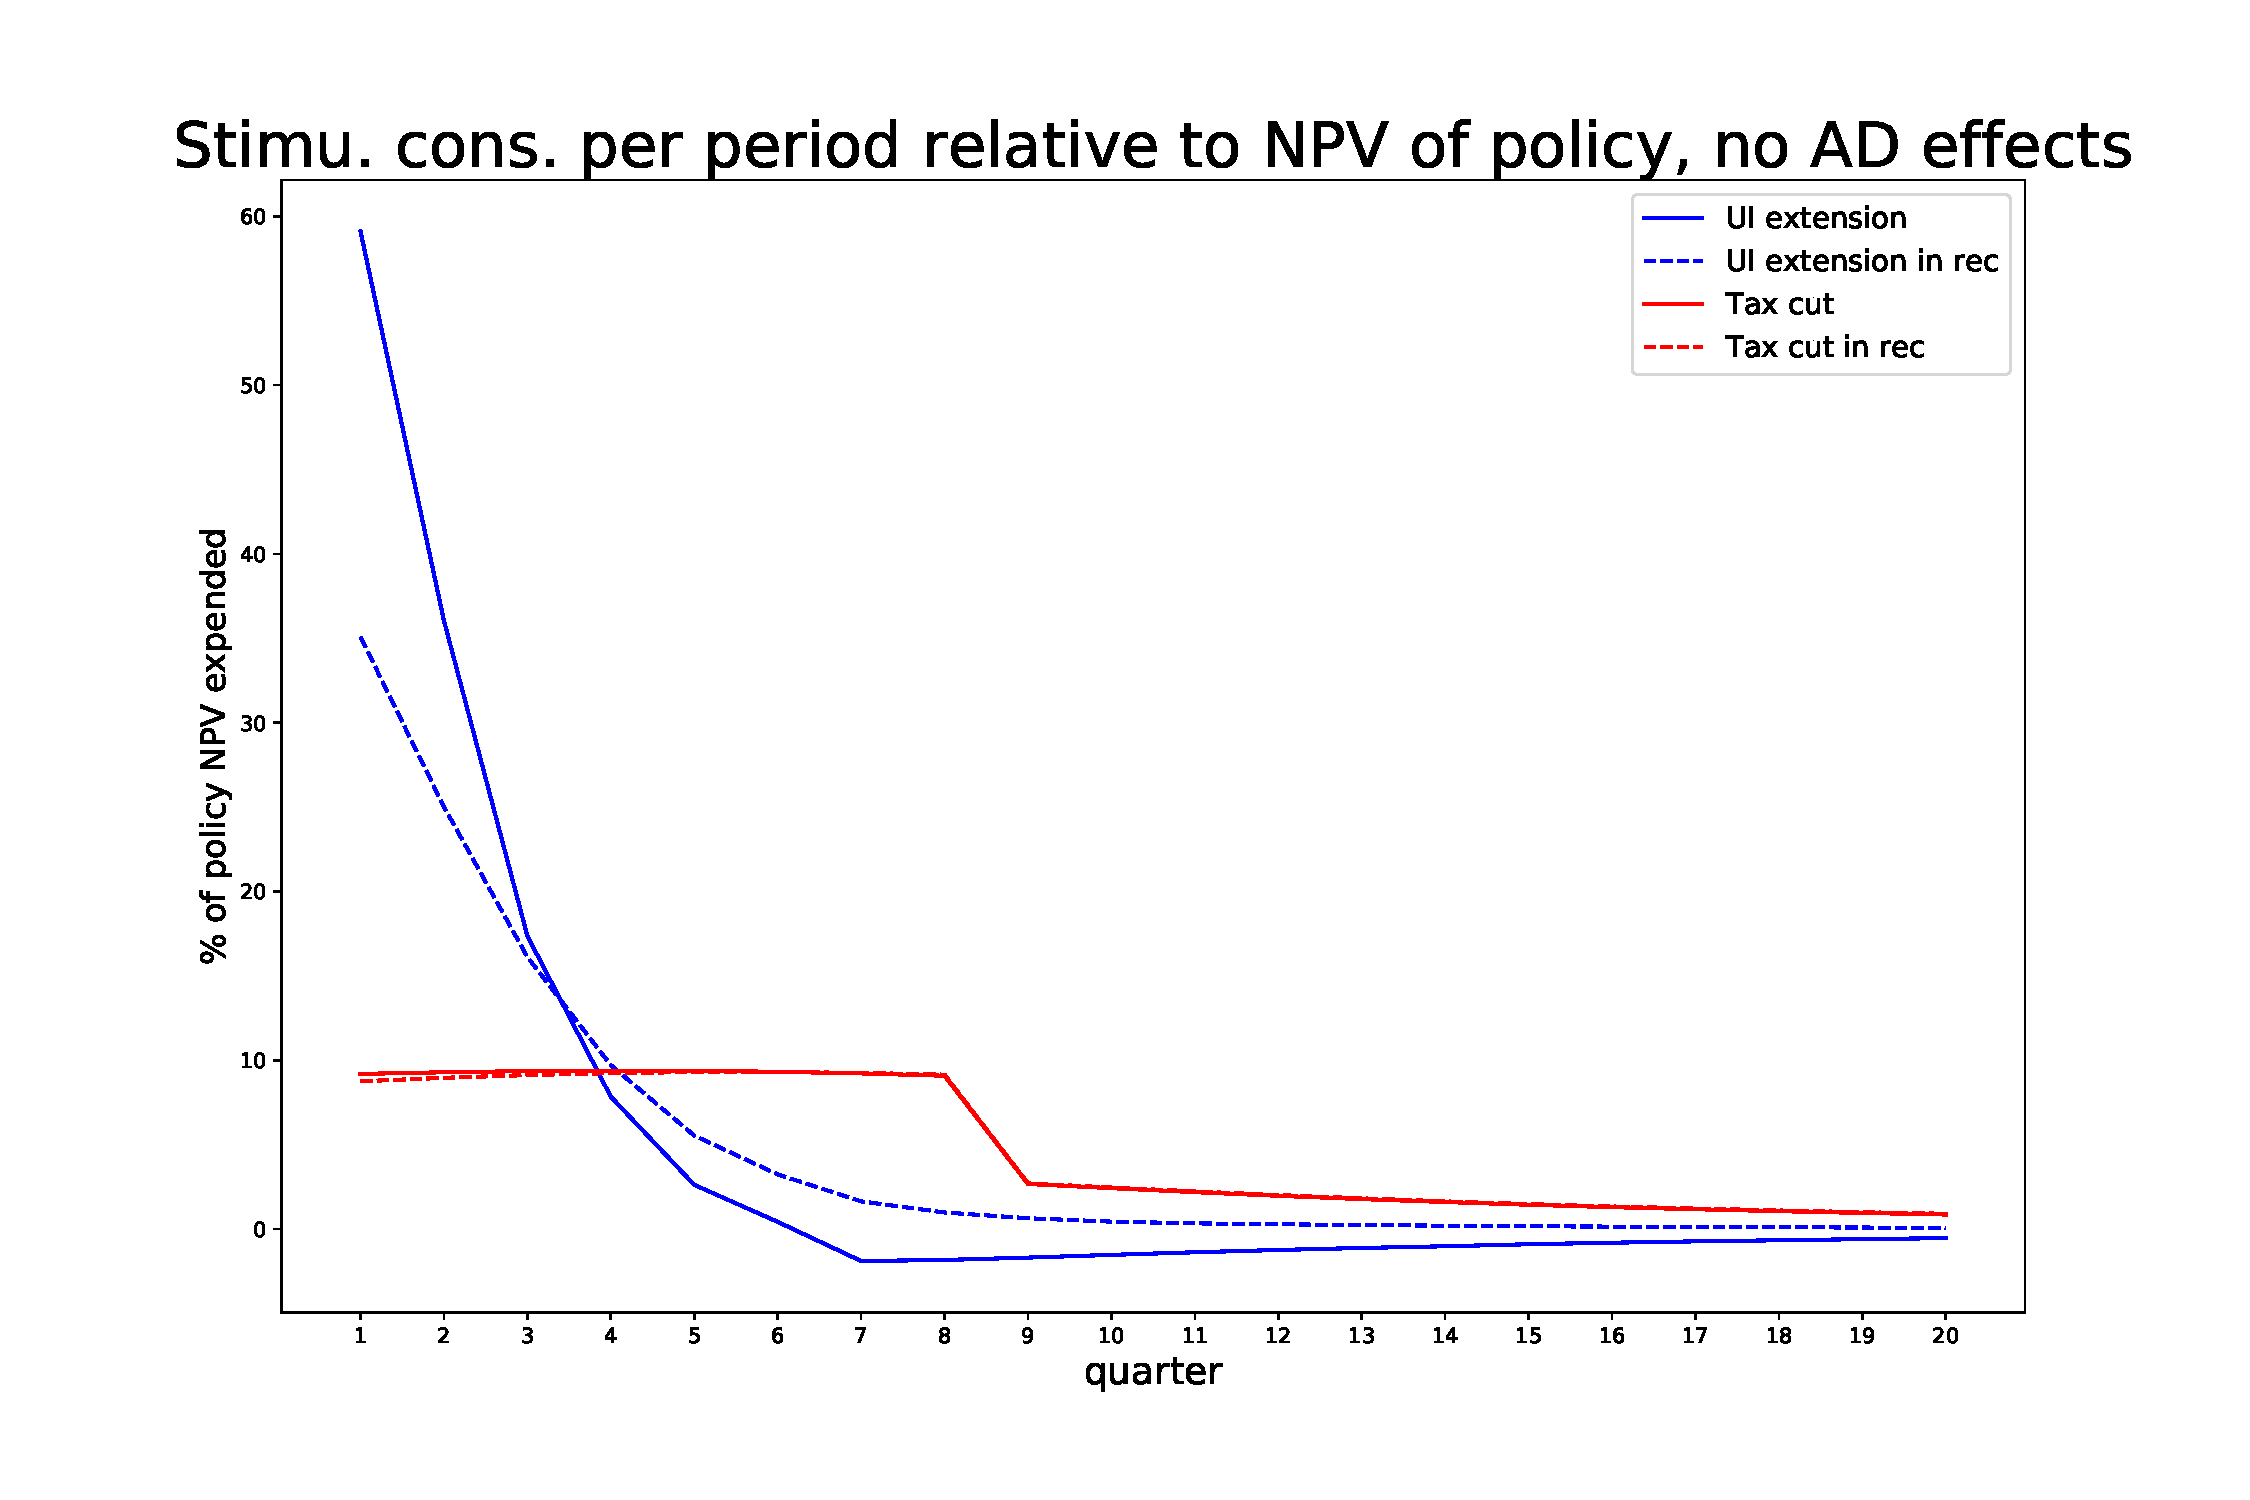
\includegraphics[width=\linewidth]{../Full_Run_with_UI_Ext/NPV_Multiplier_no_AD}
	\caption{}
	\label{fig:npvmultipliernoad}
\end{figure}


\begin{figure}
	\centering
	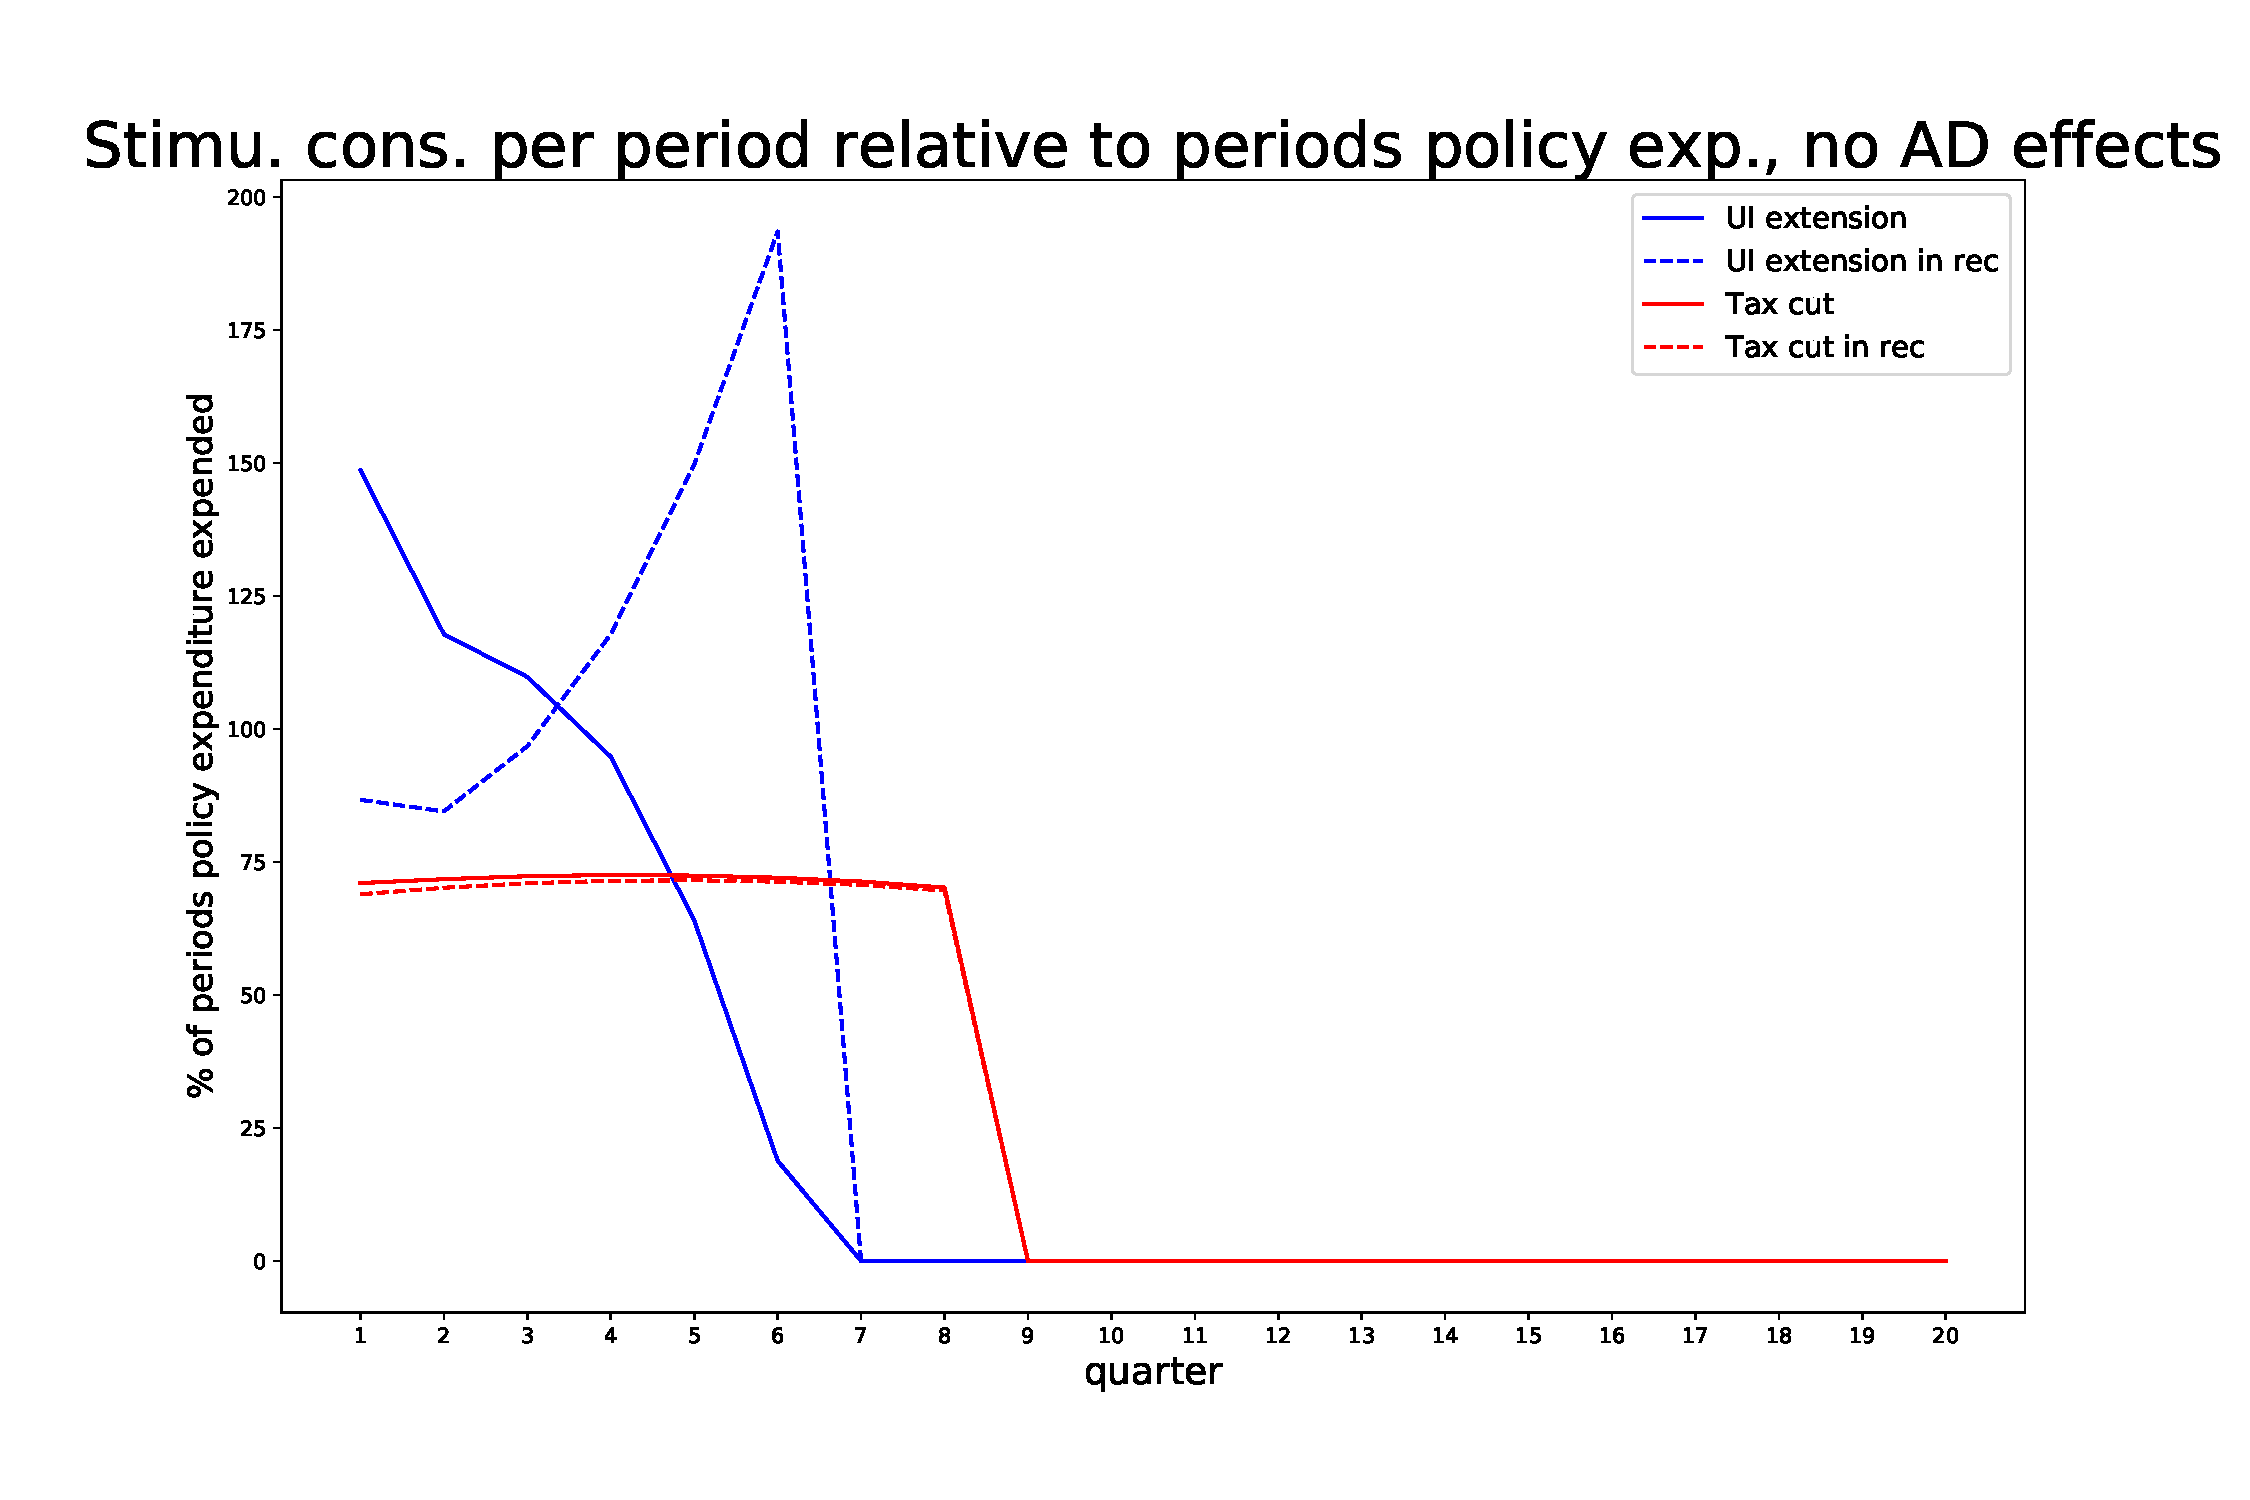
\includegraphics[width=\linewidth]{../Full_Run_with_UI_Ext/Period_Multiplier_no_AD}
	\caption{}
	\label{fig:periodmultipliernoad}
\end{figure}


\FloatBarrier
\subsection{Continuation probability linked to business cycle state}
\begin{itemize}
	\item Figure \ref{fig:taxcutrecessionnoadeffects}: No AD effects
	\item Consider either 8q or 16 tax cut (black lines)
	\item Simulations: Conditional on recesssion lasting at least 9q (otherwise: probability of continuation only when recession in q8 is meaningless.)
	\item Consumption in the case of tax cut only occuring 8q long
	\subitem - Blue:  Zero probability of continuation of tax cut after 8q
	\subitem - Green: 50\% probability of continuation of tax cut after 8q (independent of business cycle)
	\subitem - Red:   50\% probability of continuation of tax cut after 8q only when recession in q8: This curve is upward sloping as with the recession staying on it becomes more and more likely that tax cut will be extended
	\item Consumption in the case of tax cut being continued after q8
	\subitem - Green:  50\% probability of continuation of tax cut after 8q (independent of business cycle)
	\subitem - Red:    50\% probability of continuation of tax cut after 8q only when recession in q8
	\subitem - Orange: 100\% probability of continuation of tax cut after 8q only when recession in q8
	\item Conclusion: Continuing the payroll tax cut even when recession ends does not boost consumption by much (except during first quarters) (see diff red green line). More stimulating is a guarantee to extend the tax cut in case of an ongoing recession.
	\item Figure \ref{fig:taxcutrecessionadeffects}: same but with AD effects
\end{itemize}
	
\begin{figure}
	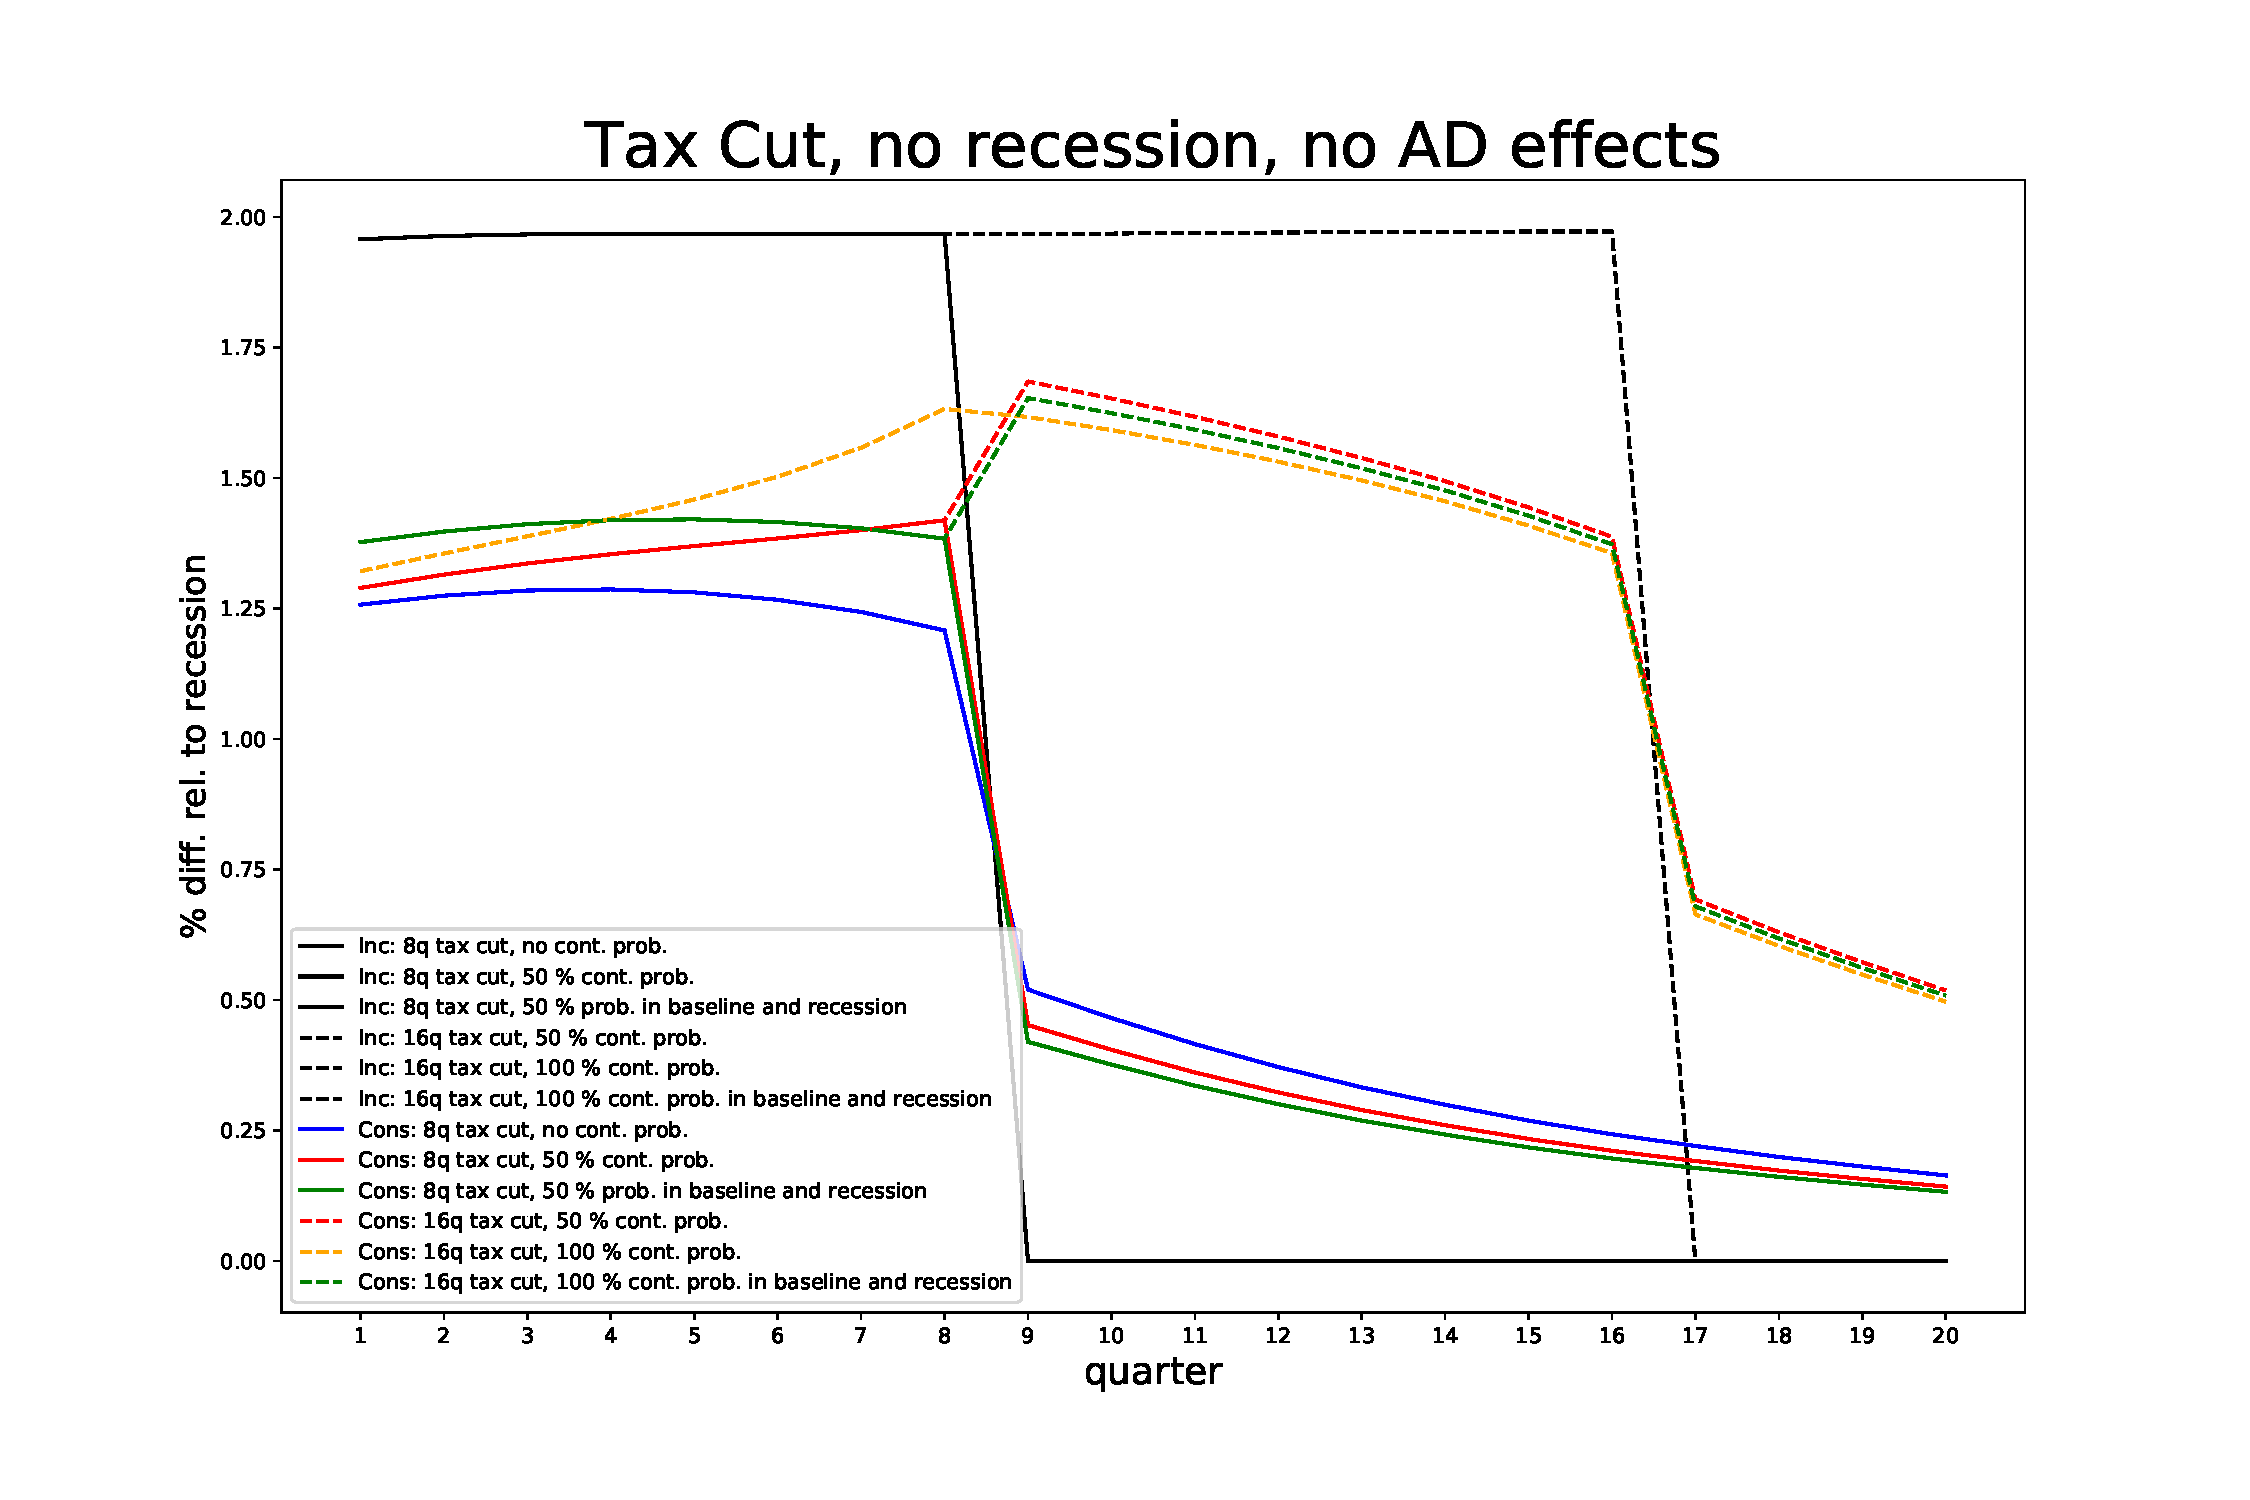
\includegraphics[width=1\linewidth]{../Continuation_Prob_Experiments/tax_cut_recession_no_AD_effects}
	\caption{}
	\label{fig:taxcutrecessionnoadeffects}
\end{figure}
	
\begin{figure}
	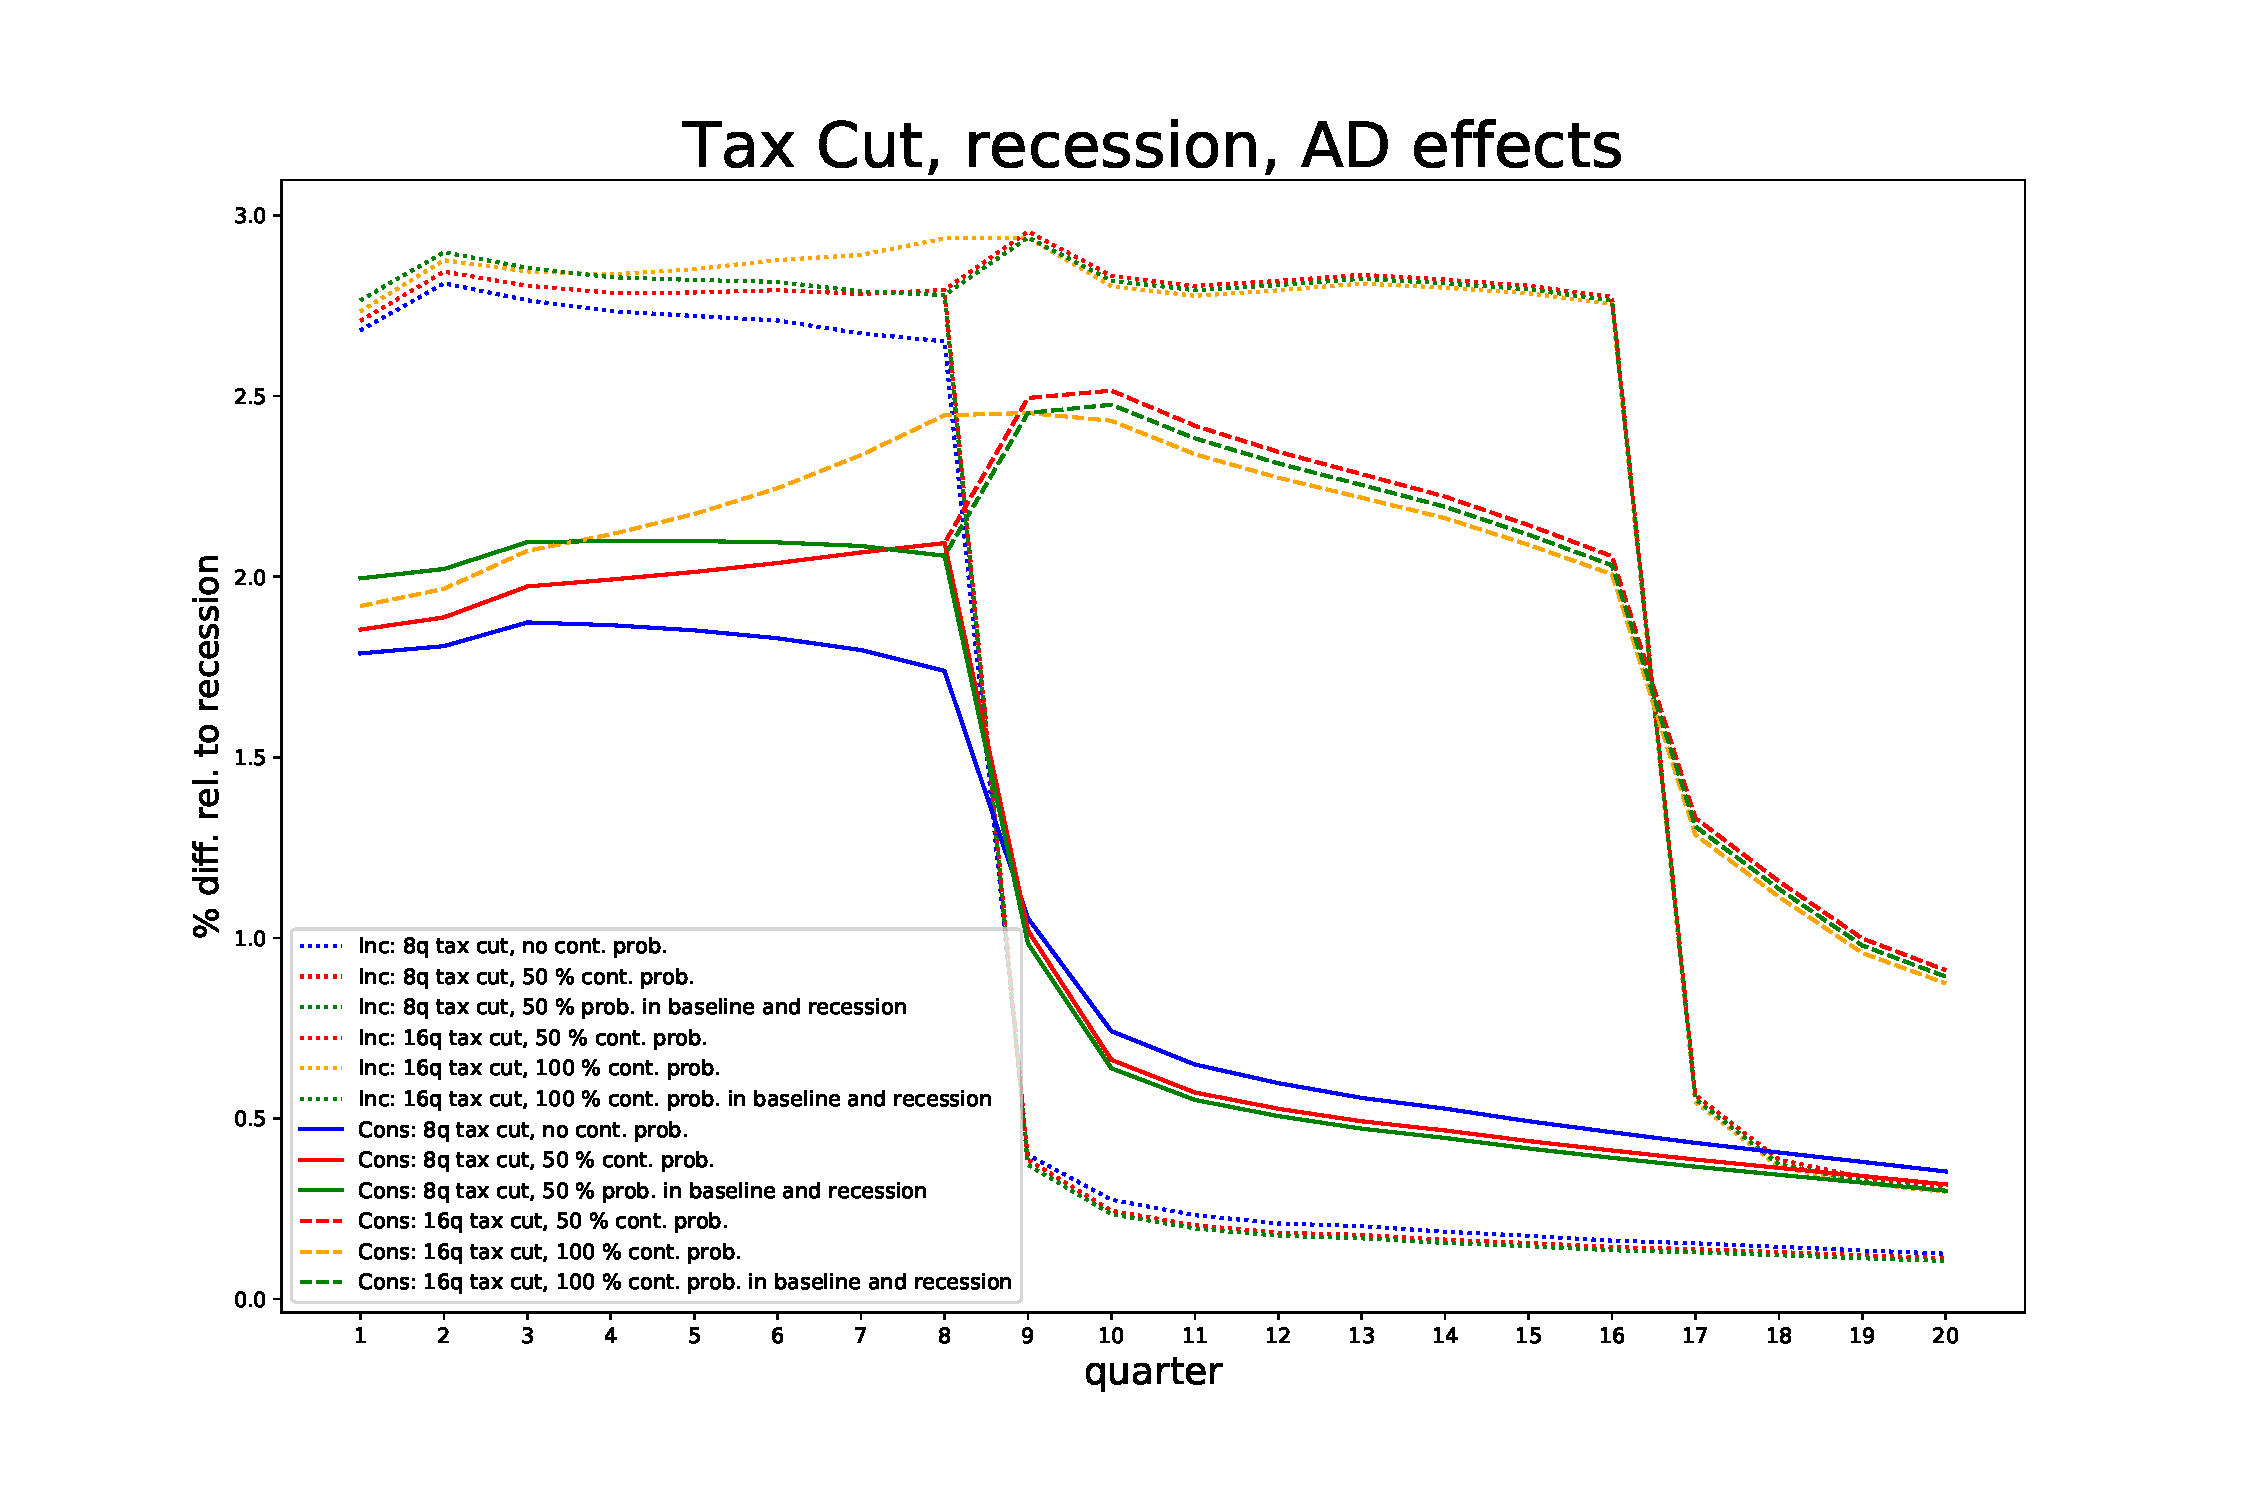
\includegraphics[width=1\linewidth]{../Continuation_Prob_Experiments/tax_cut_recession_AD_effects}
	\caption{}
	\label{fig:taxcutrecessionadeffects}
\end{figure}
	
	
	
	
	
\FloatBarrier
\section{Update - February 10th 2021}	


\FloatBarrier	
\subsection{Improved convergence}

\FloatBarrier
\subsection{Tax cut}

\begin{figure}
	\centering
	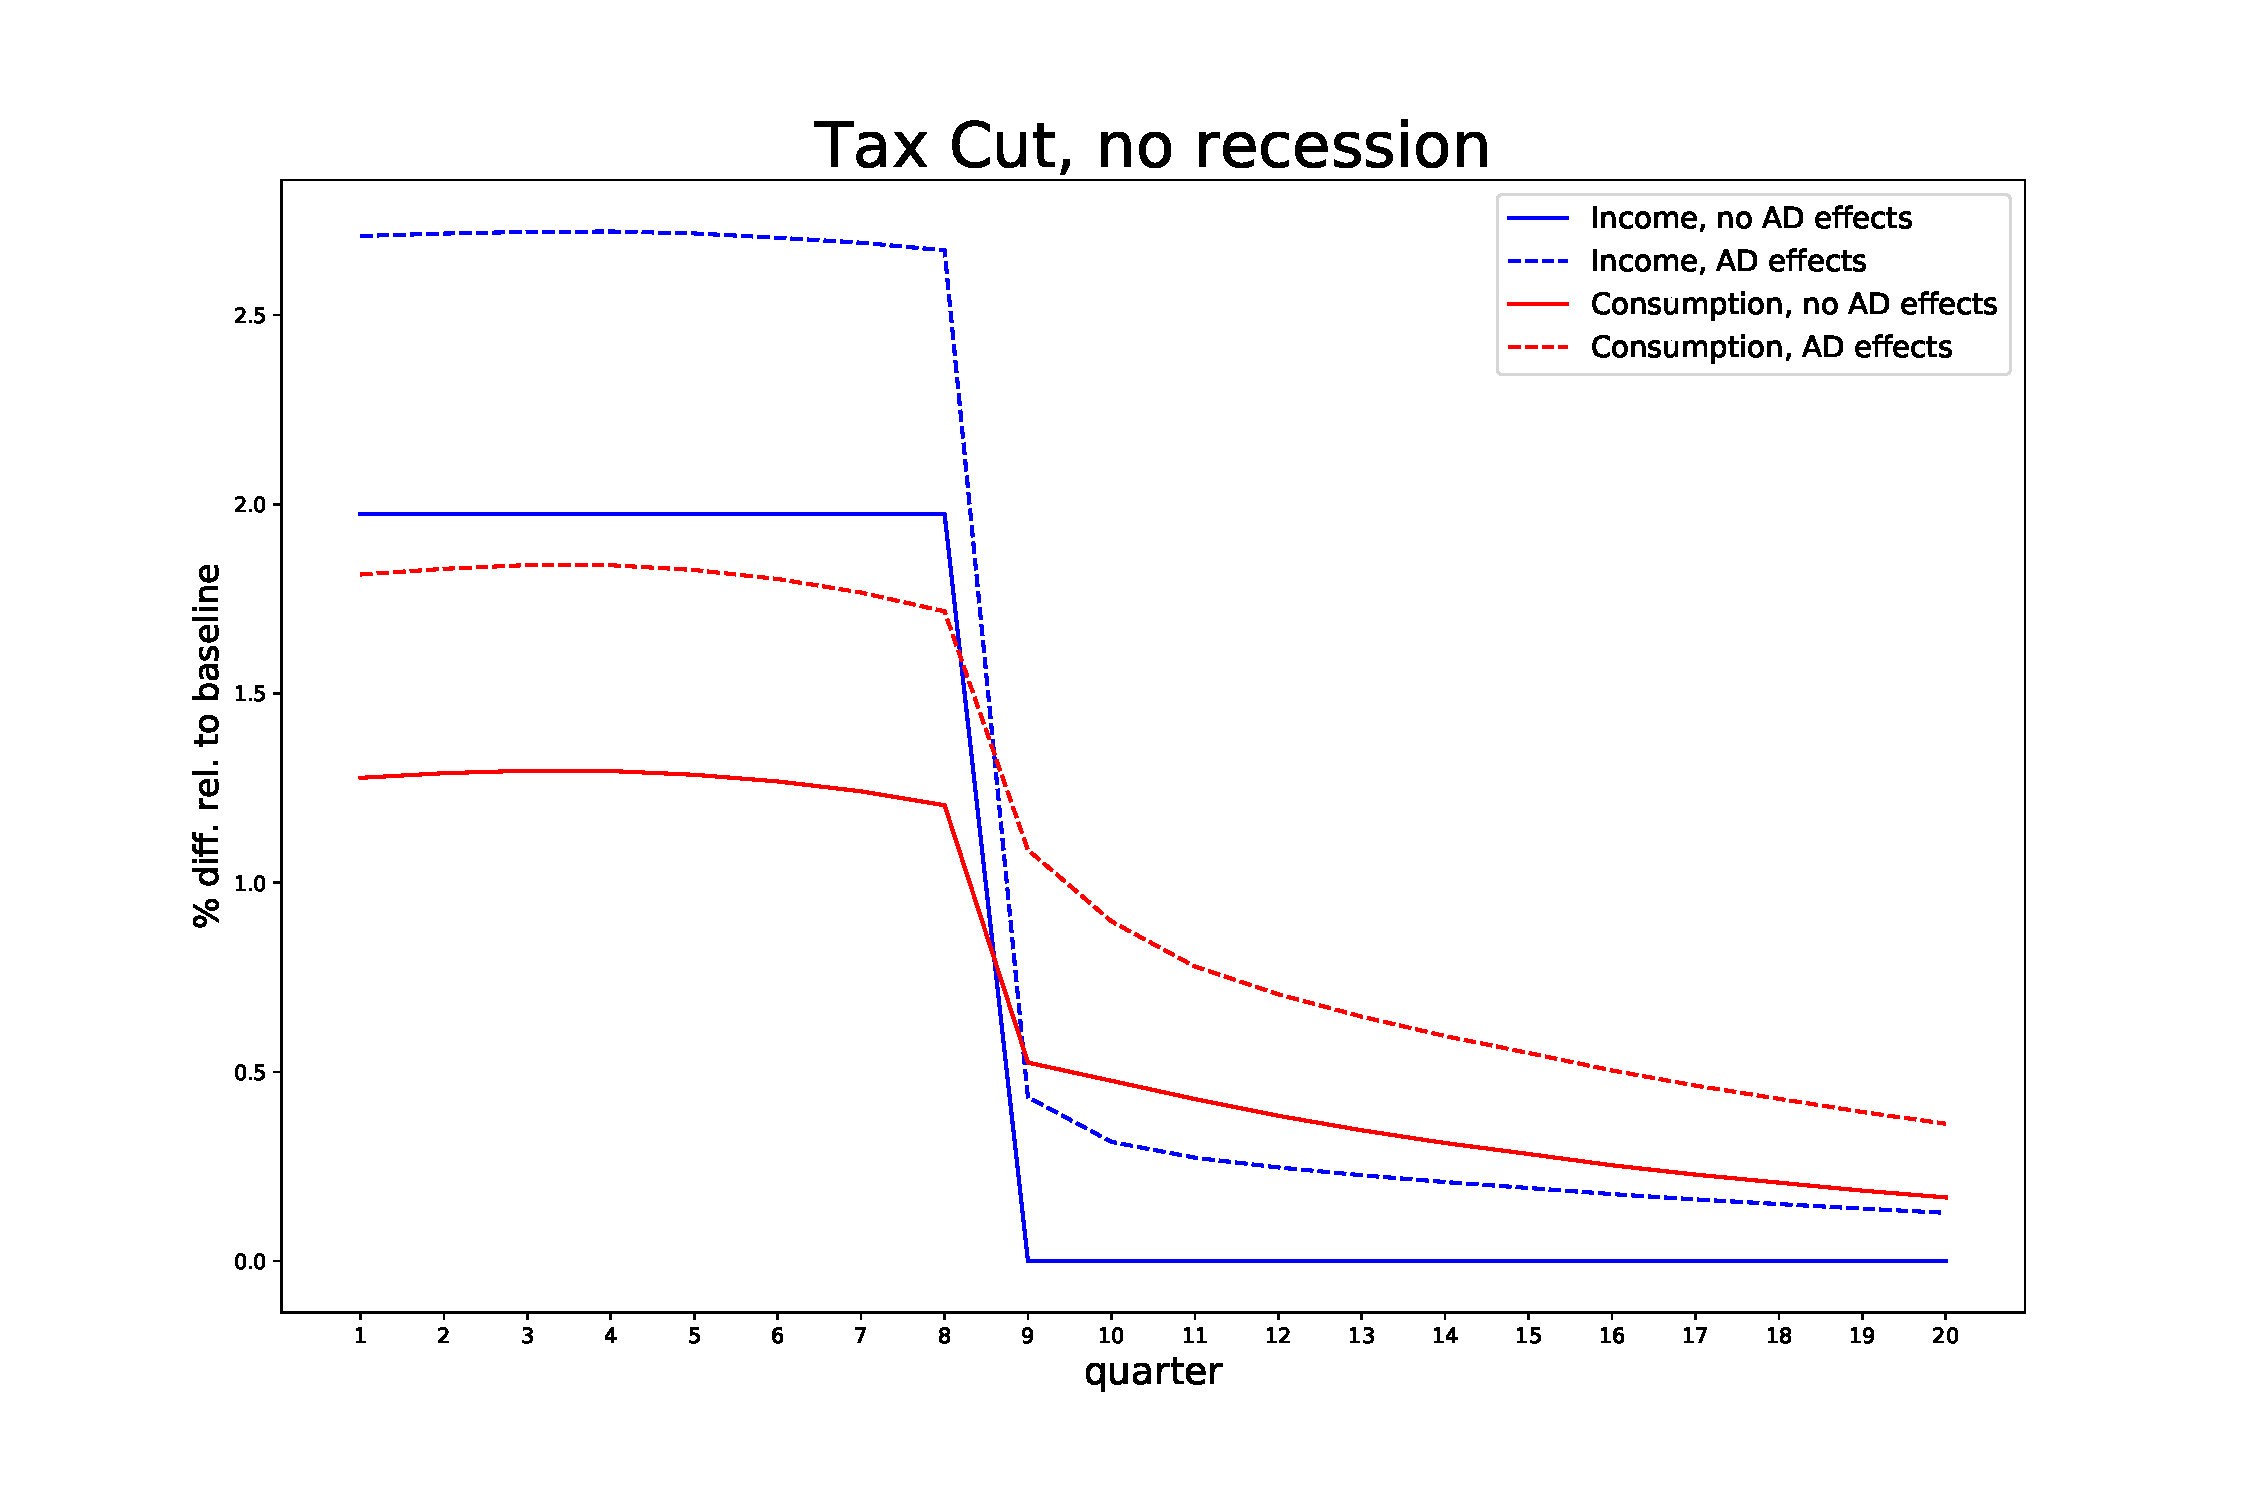
\includegraphics[width=\linewidth]{../full_run/tax_cut}
	\caption{}
	\label{fig:taxcut}
\end{figure}
\begin{figure}
	\centering
	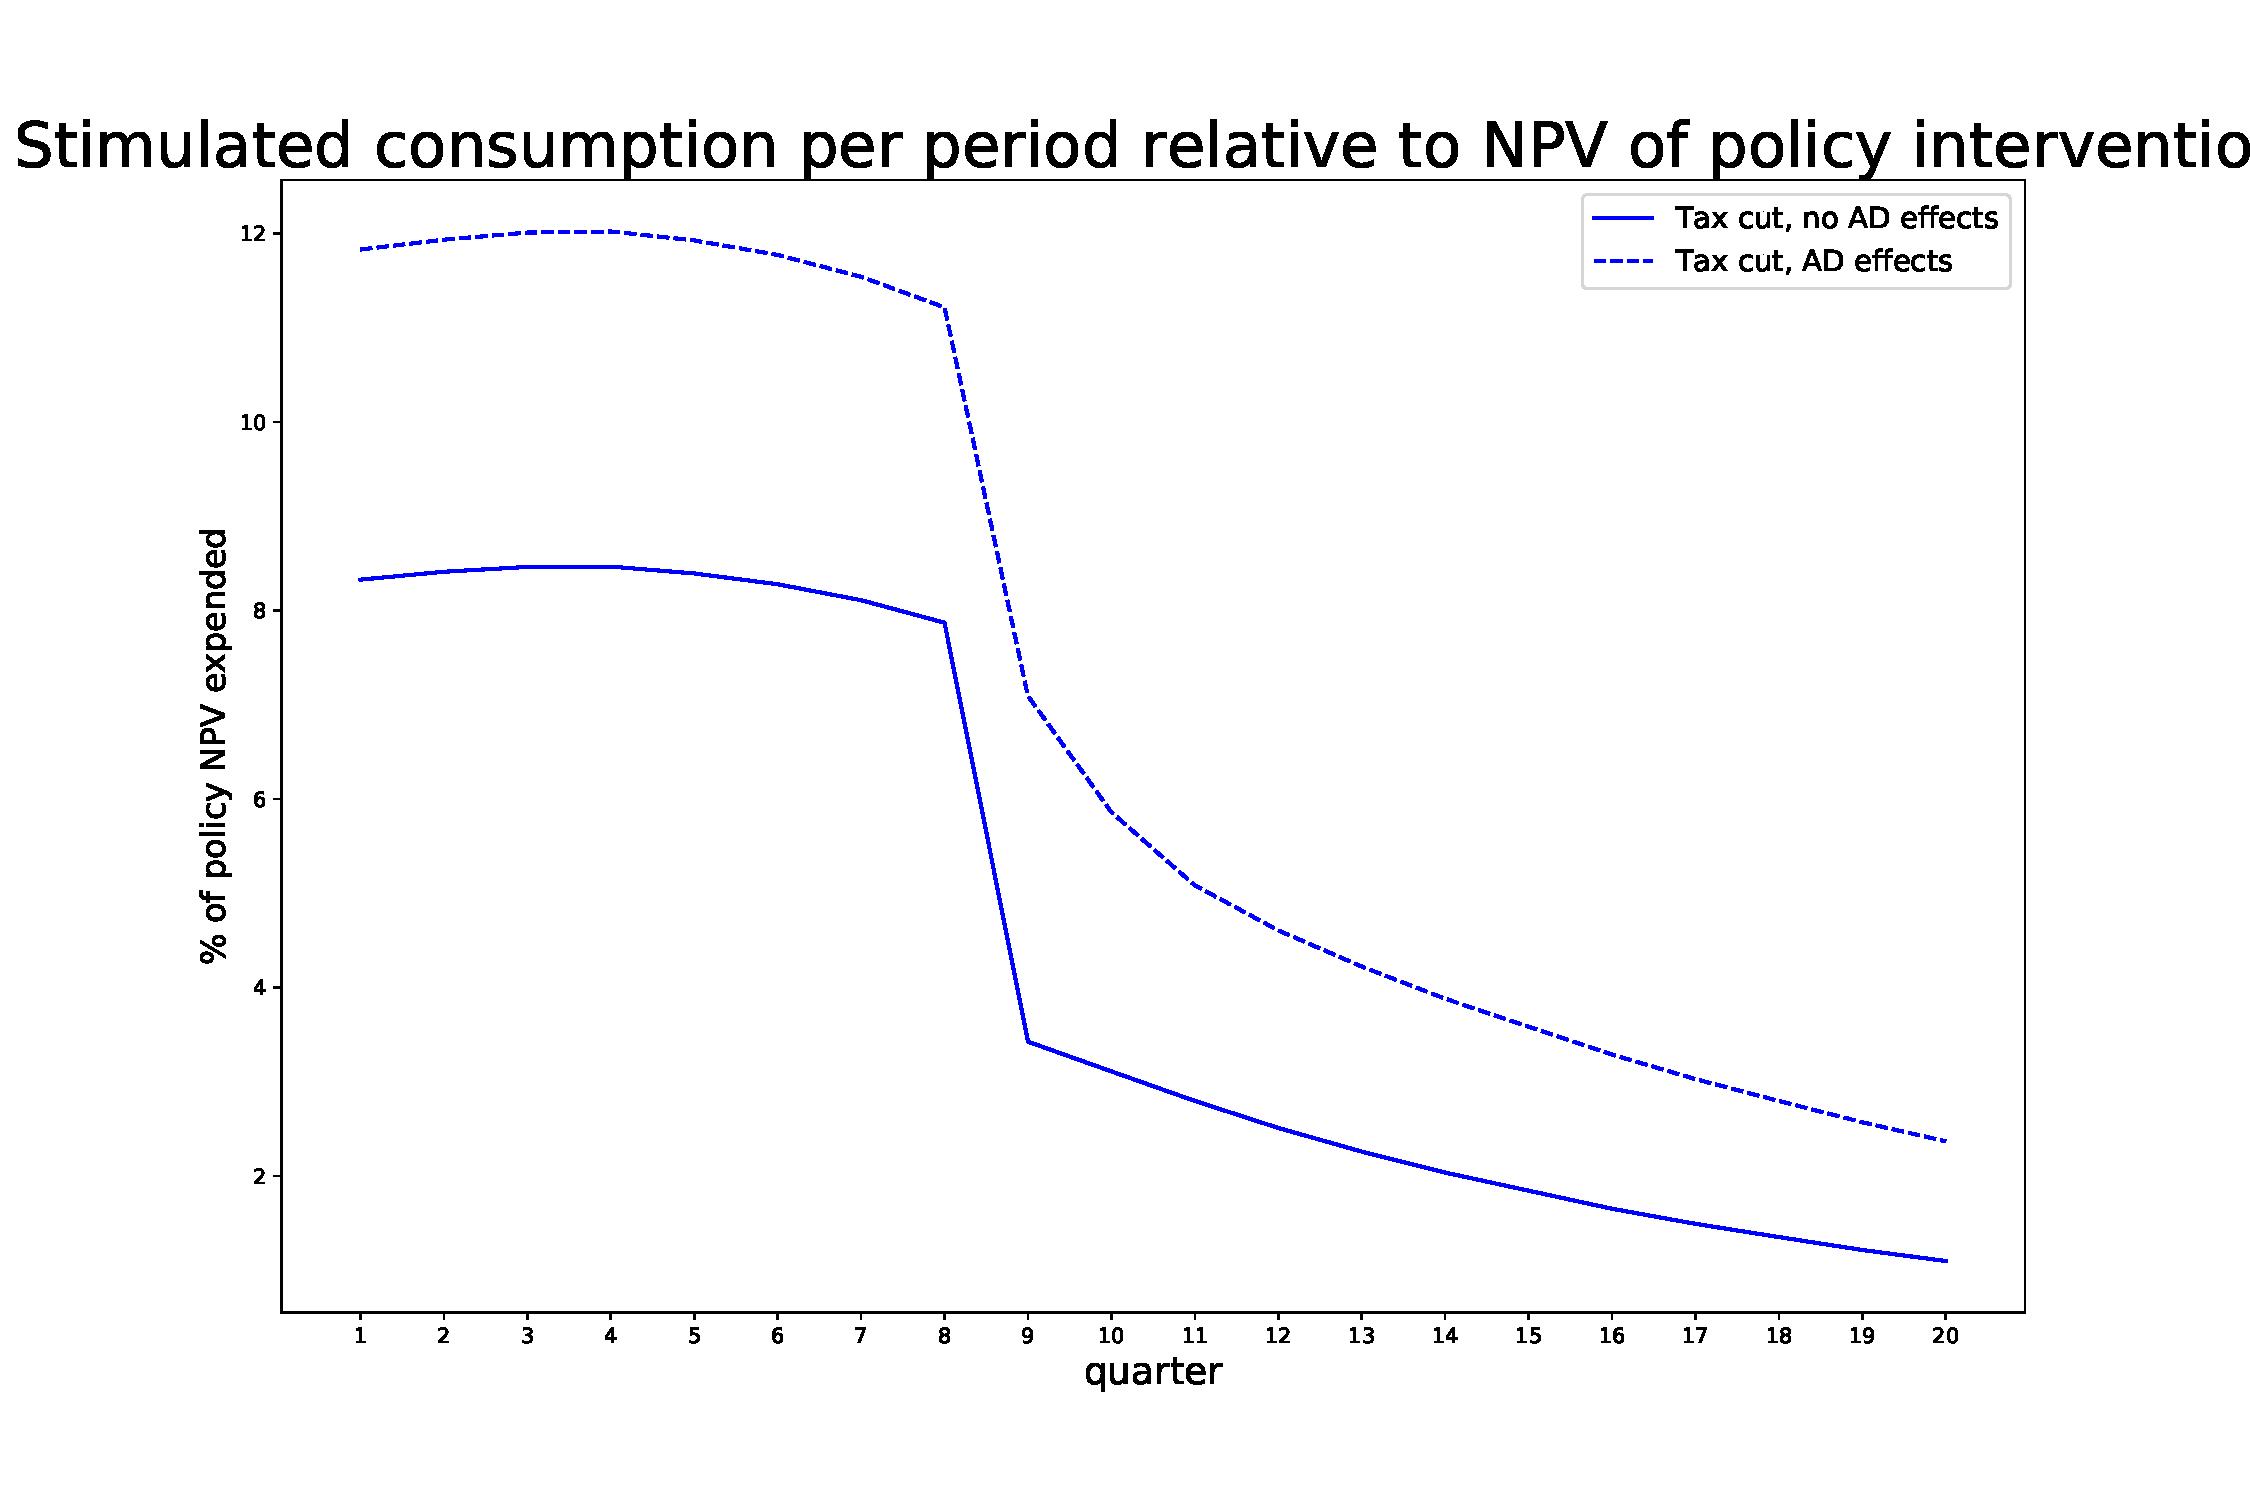
\includegraphics[width=\linewidth]{../full_run/stimulated-consumption_TaxCut}
	\caption{}
	\label{fig:stimulated-consumptiontaxcut}
\end{figure}


\begin{itemize}
	\item We consider a payroll tax cut by 2 pp for 8q (deterministic length)
	\item See Figure \ref{fig:taxcut}
	\subitem The tax increases income and consequently pushes up consumption
	\subitem The drop in consumption in 9q is due to the fact that the splurge is applied to income in excess of the baseline income, which drops to zero after the tax cut is reversed. Consumption spending remains elevated for some time after the tax cut due to built up savings. 
	\subitem With aggregate demand effects, the effect on consumption is larger as the increased consumption reinforces consumption through higher income due to higher TFP	
\end{itemize}

\FloatBarrier
\subsubsection{Recession}

\begin{figure}
	\centering
	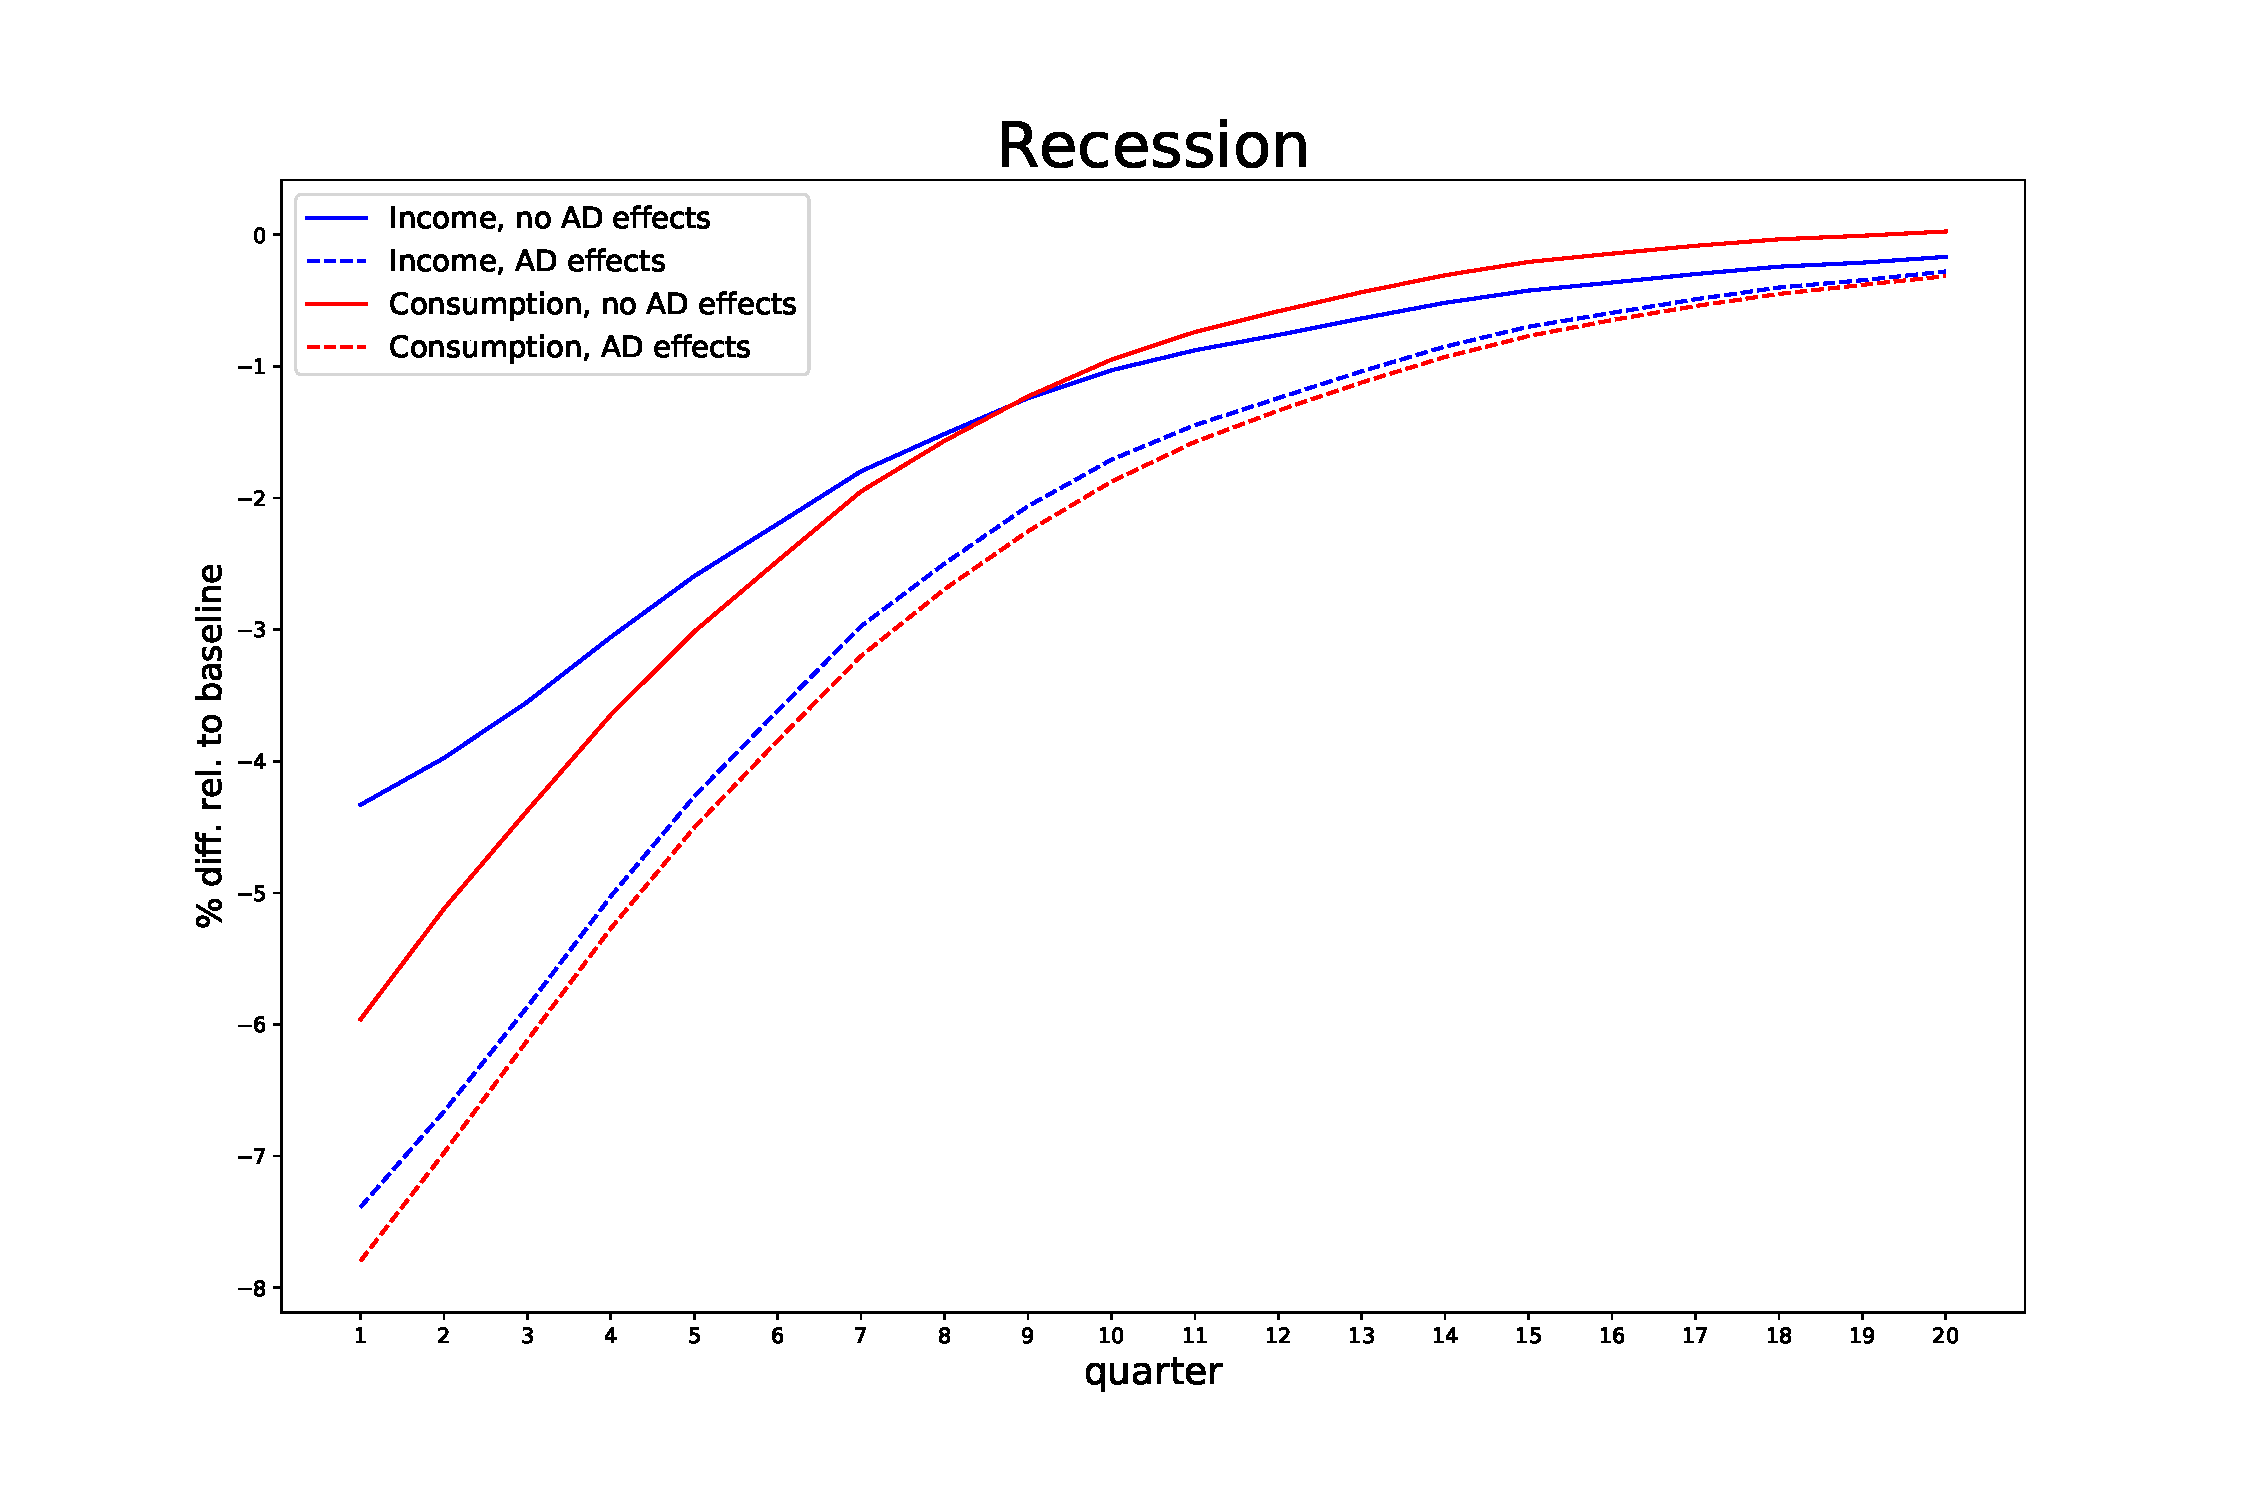
\includegraphics[width=\linewidth]{../full_run/recession}
	\caption{}
	\label{fig:recession}
\end{figure}


\begin{itemize}
	\item We consider a recession with an expected length of 6 quarters, see Figure \ref{fig:recession}
	\item In a recession the unemployment rate increases to 10 \% and lasts on average 4 quarters (as opposed to 5\% / 1.5 q in normal times)
	\item The recession depresses aggregate income due to loss of labor income, only partly compensated by unemployment benefits (lasting 2 q, replacing 30 \% of income)
	\item Consumption falls as income is lower.
	\item The recession is deeper when productivity depends on aggregate demand.
\end{itemize}




\FloatBarrier
\subsection{Tax cut during recession}


\begin{figure}
	\centering
	\begin{subfigure}[b]{\textwidth}
		\centering
		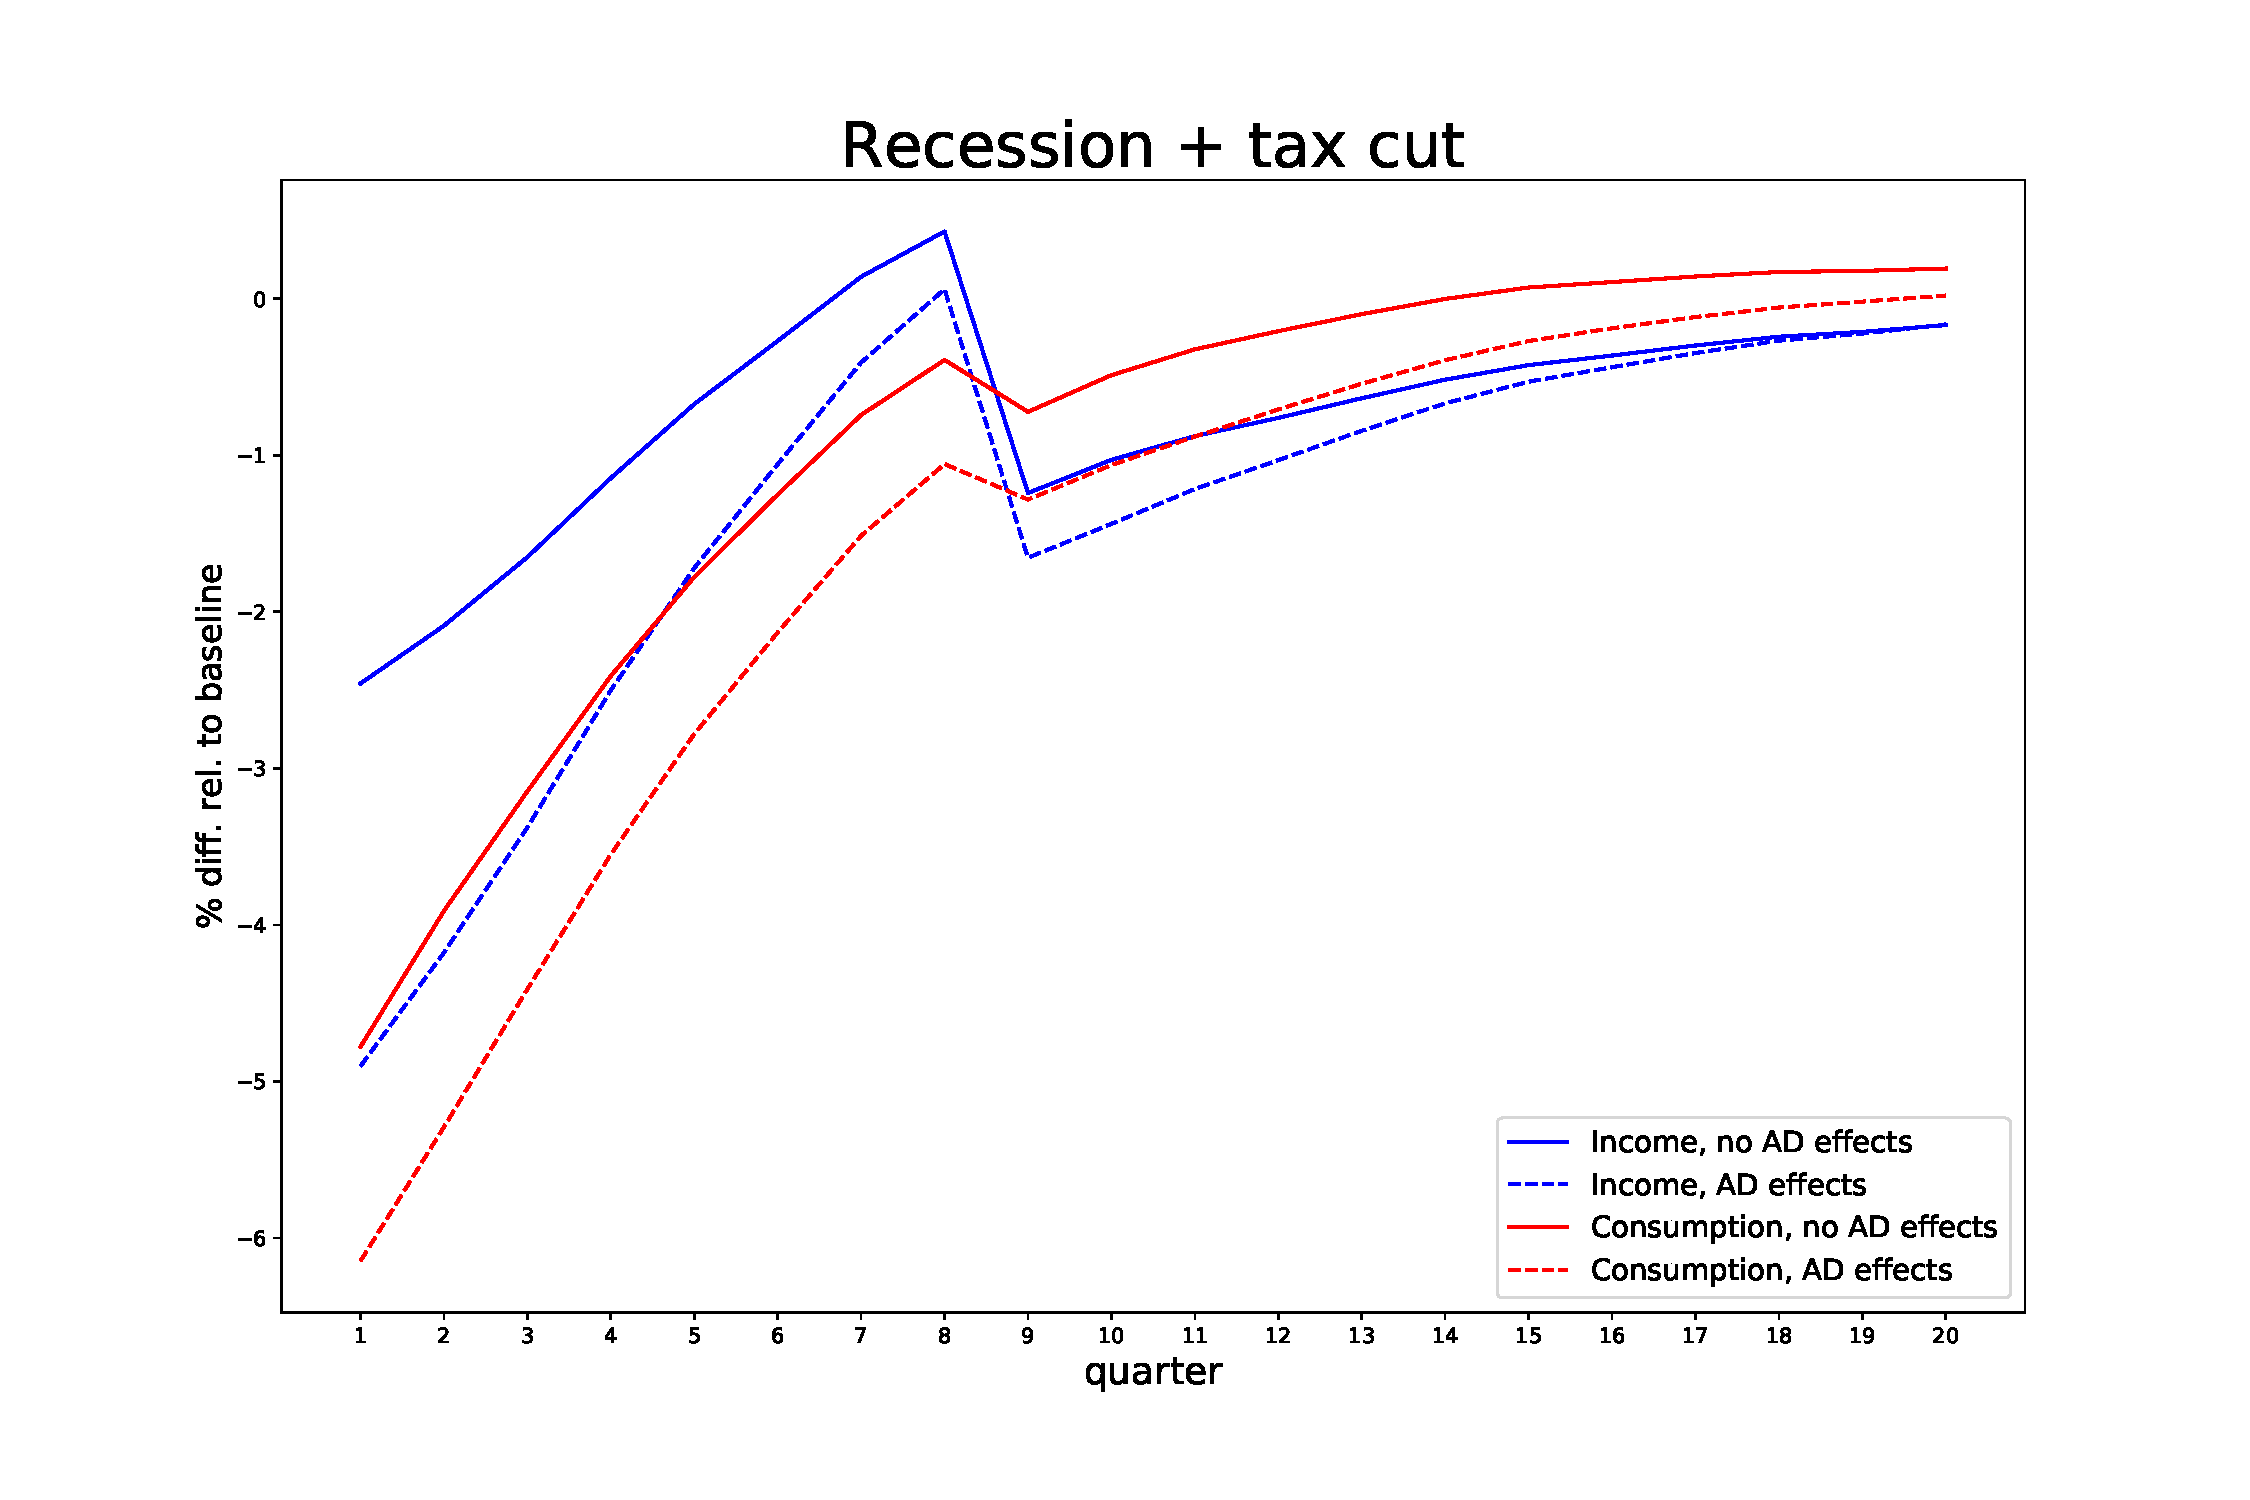
\includegraphics[width=\linewidth]{../full_run/recession_taxcut_relbaseline}
		\caption{rel. to baseline}
		\label{fig:recessiontaxcutrelbaseline}
	\end{subfigure}\\
	\hfill
	\begin{subfigure}[b]{\textwidth}
	\centering
	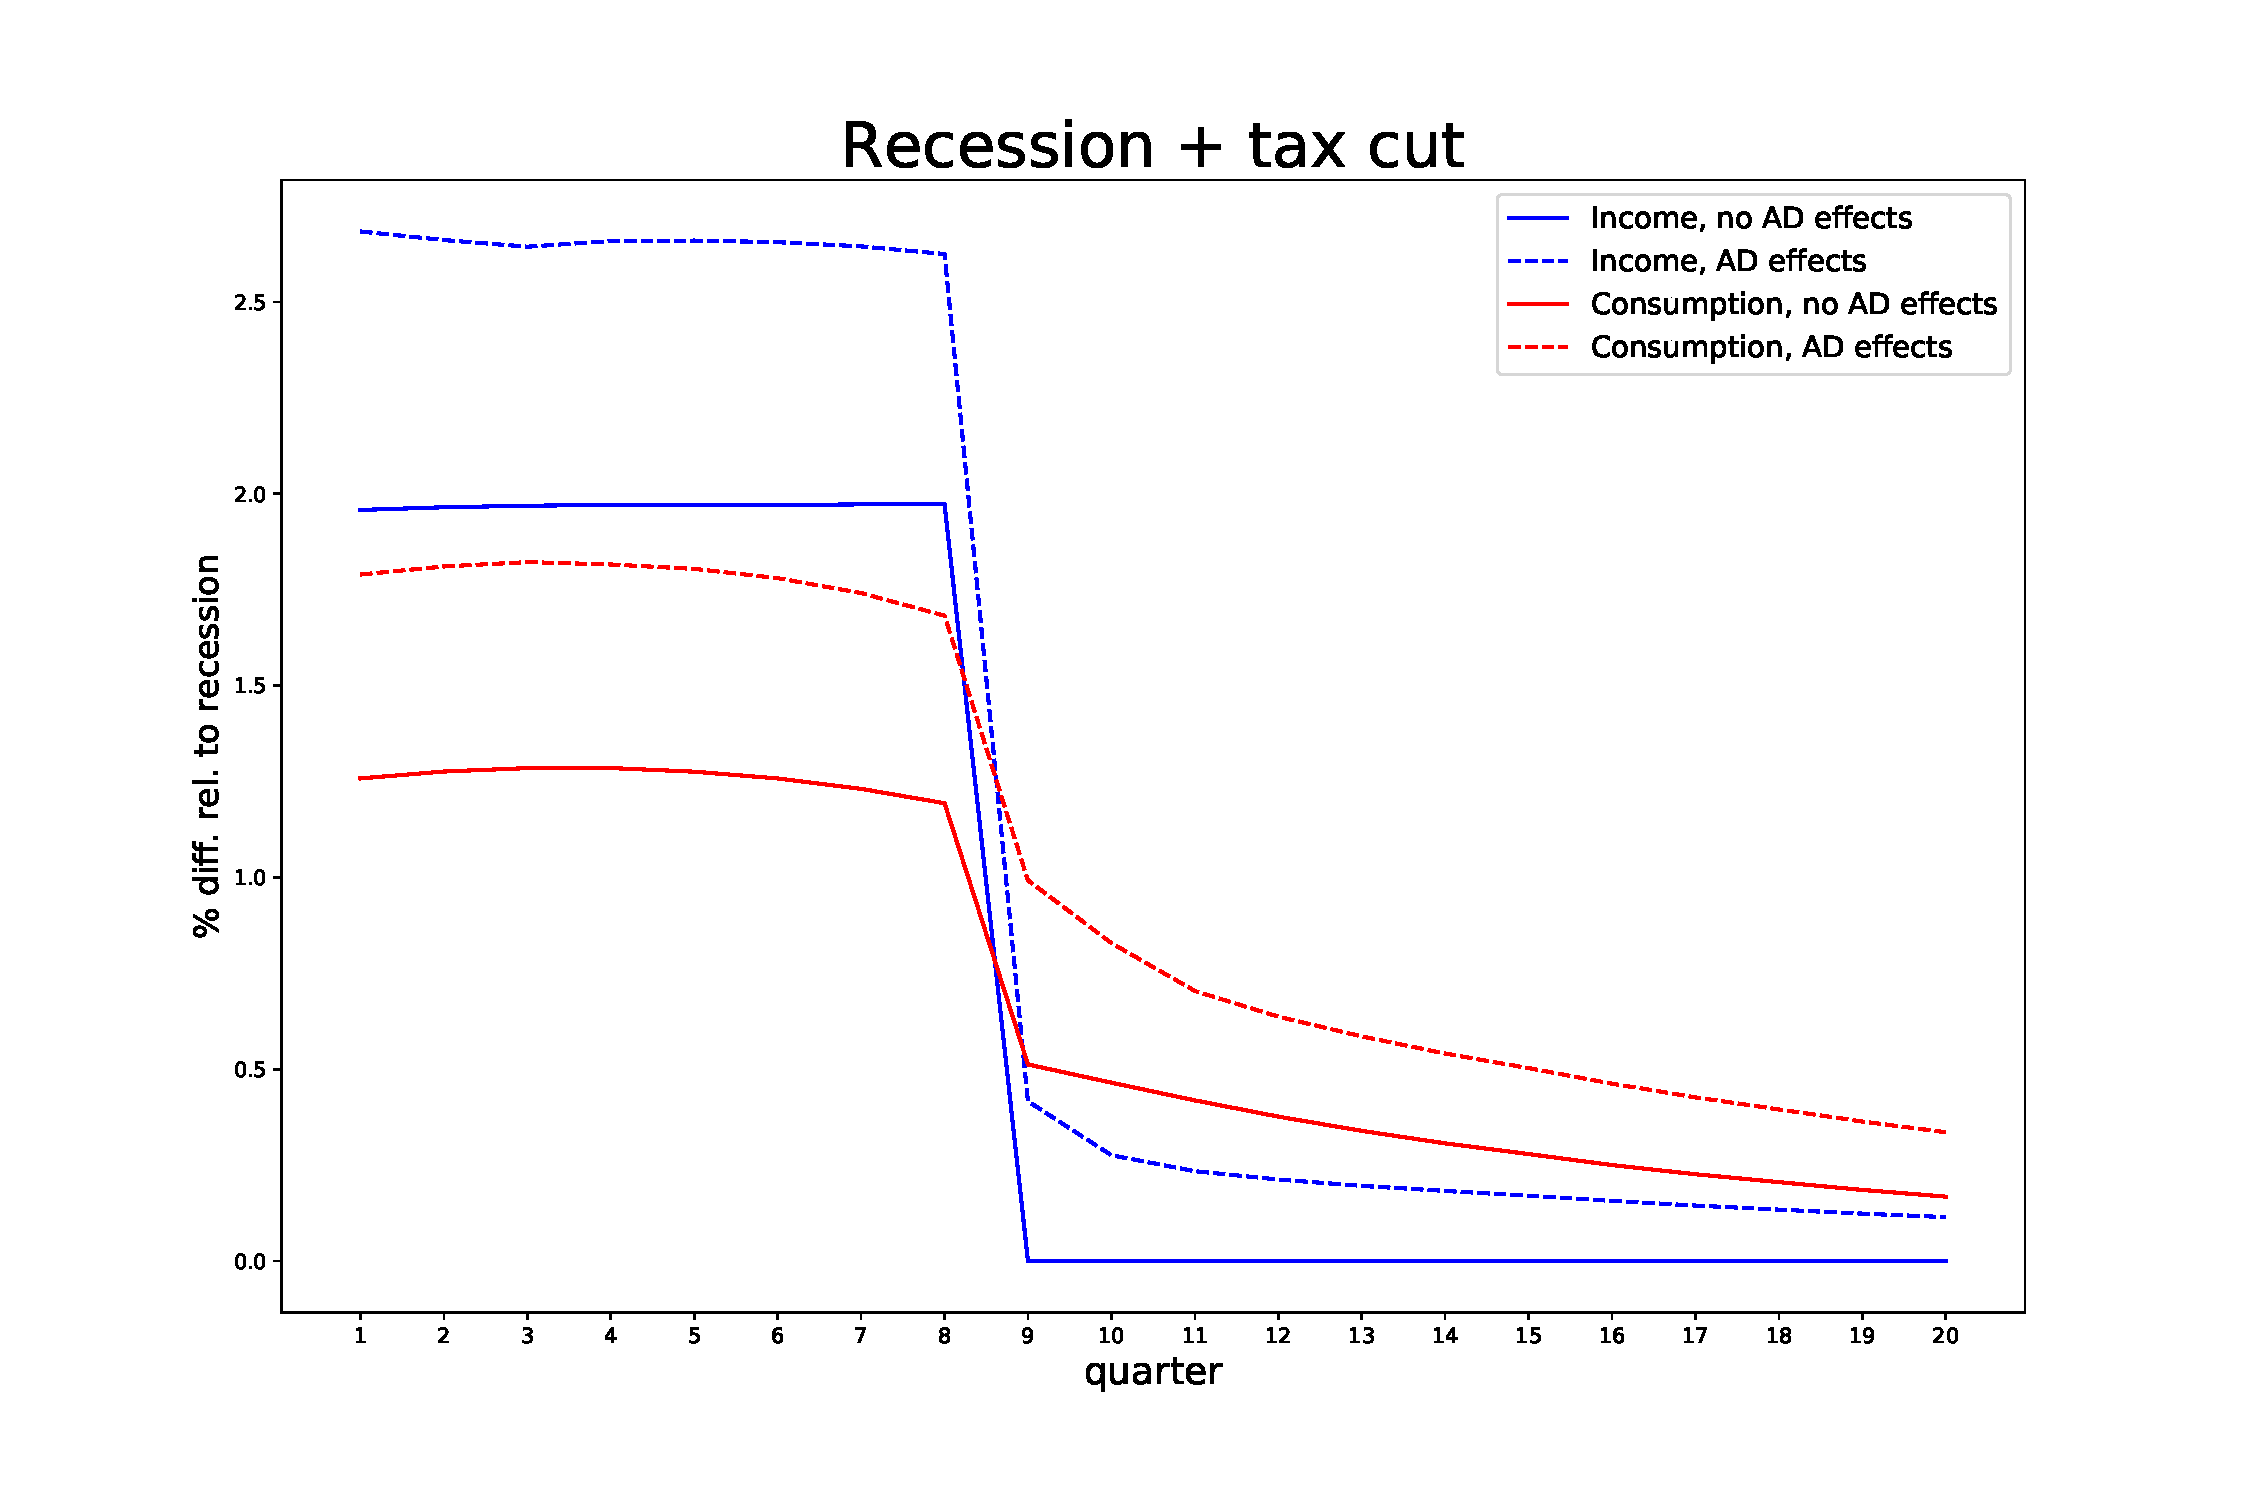
\includegraphics[width=\linewidth]{../full_run/recession_taxcut_relrecession}
	\caption{rel. to recession}
	\label{fig:recessiontaxcutrelrecession}
	\end{subfigure}
\end{figure}

\begin{figure}
	\centering
	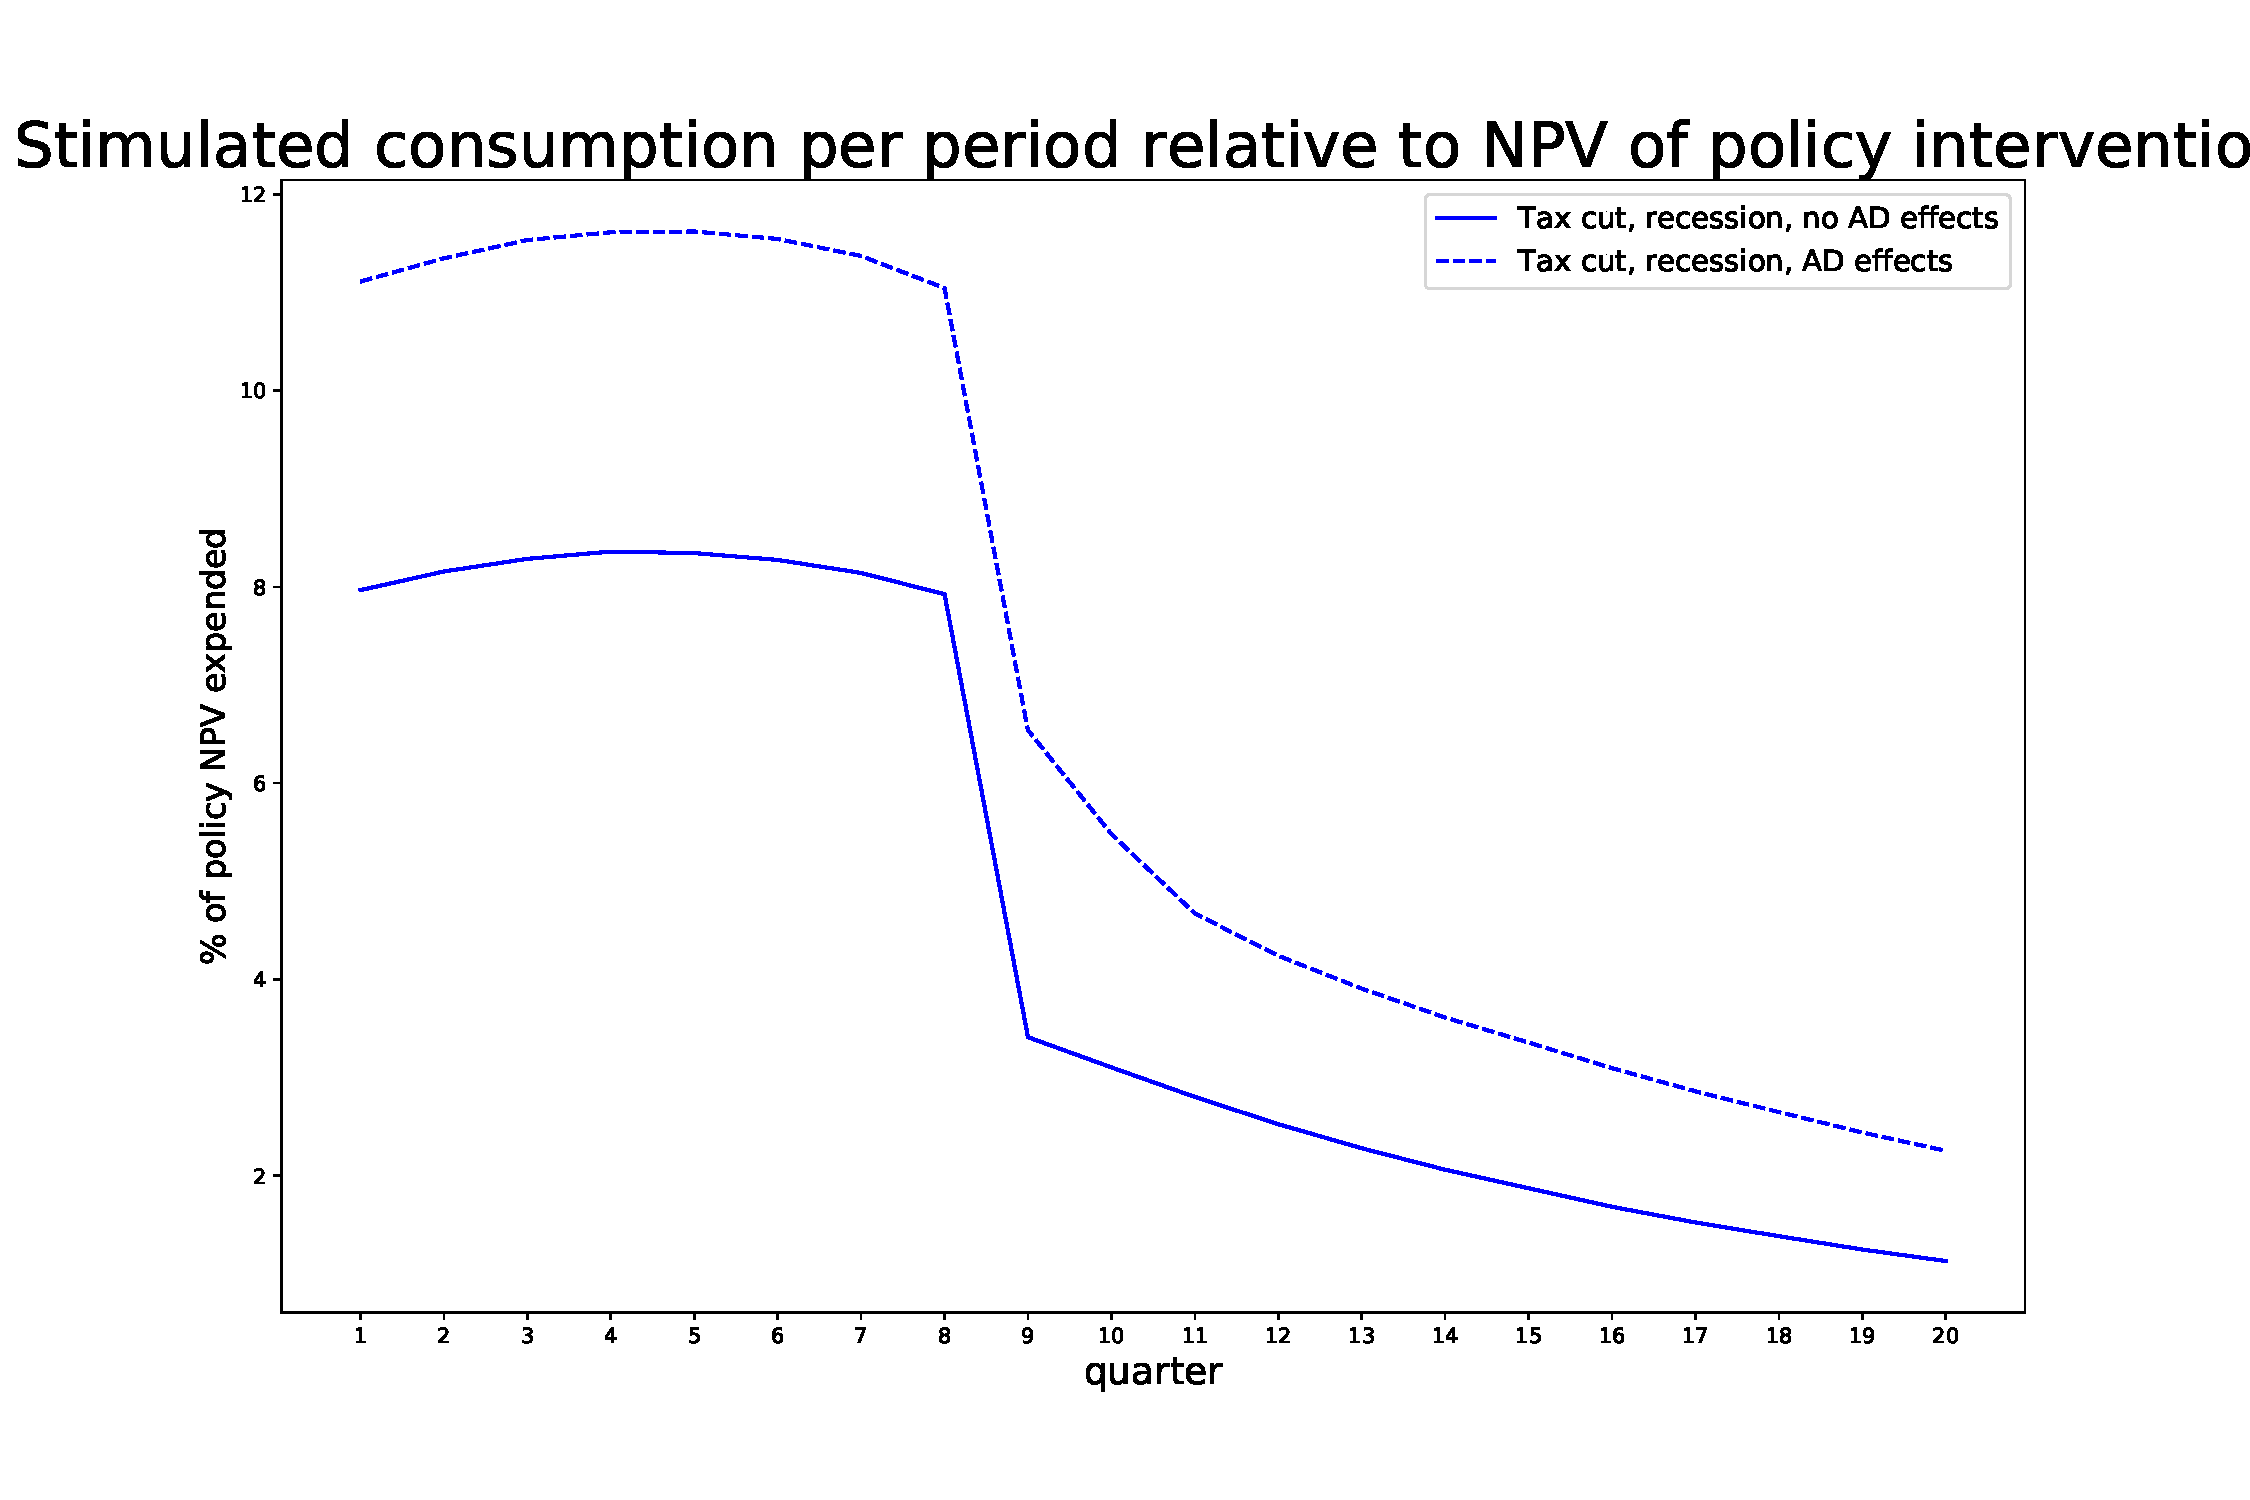
\includegraphics[width=\linewidth]{../full_run/stimulated-consumption_RecTaxCut}
	\caption{}
	\label{fig:stimulated-consumptionrectaxcut}
\end{figure}



\begin{itemize}
	\item We consider a payroll tax cut by 2 pp for 8q (deterministic length) during a recession with an expected length of 6q 
	\item Additional income / consumption relative to the baseline (see figure \ref{fig:taxcutrecession}) and to recession scenario (see figure \ref{fig:taxcutrecession2})
	\item When AD effects are switched off we obtain a similar result as in the baseline. However, note, that as the recession disappears, the additional income by the tax cut increases as more people are employed
	\item This upward trend in the effect of the tax cut is much more pronounced when considering AD effects. This is because very low consumption at the beginnning of the recession sets a much steeper recovery path.
	\item Not clear why consumption first drops (numerical error?)
\end{itemize}


	
\FloatBarrier	
\subsection{Deterministic length of the payroll tax cut vs. probability of continuation}

We compare a payroll tax cut (of 2 percentage points) when the length of the payroll tax cut policy is deterministic and set to eight quarters vs. when there is a 50\% chance (of which everyone is aware) of an continuation of the initial eight quarter of payroll tax cut by another eight quarters (and so on). We do so with and without aggregate demand (AD) effects.

\begin{itemize}
	\item Figure \ref{fig:taxcutnorecessionnoadeffects} shows the payroll tax cut without AD effects
	\item Income increases for either 8 or 16 q depending on scenario
	\item Consumption during the first 8q is higher when there is a chance of continuation of the policy even if it does not materialize. If it does not materialize consumption in quarter 9 falls below the level relative to the scenario where continuation was excluded out in the first place, because consumption was based on the expected income.
	\item When the continuation actually occurs, agents increase consumption because actual income exceeds expected income.
\end{itemize}

\begin{figure}
	\centering
	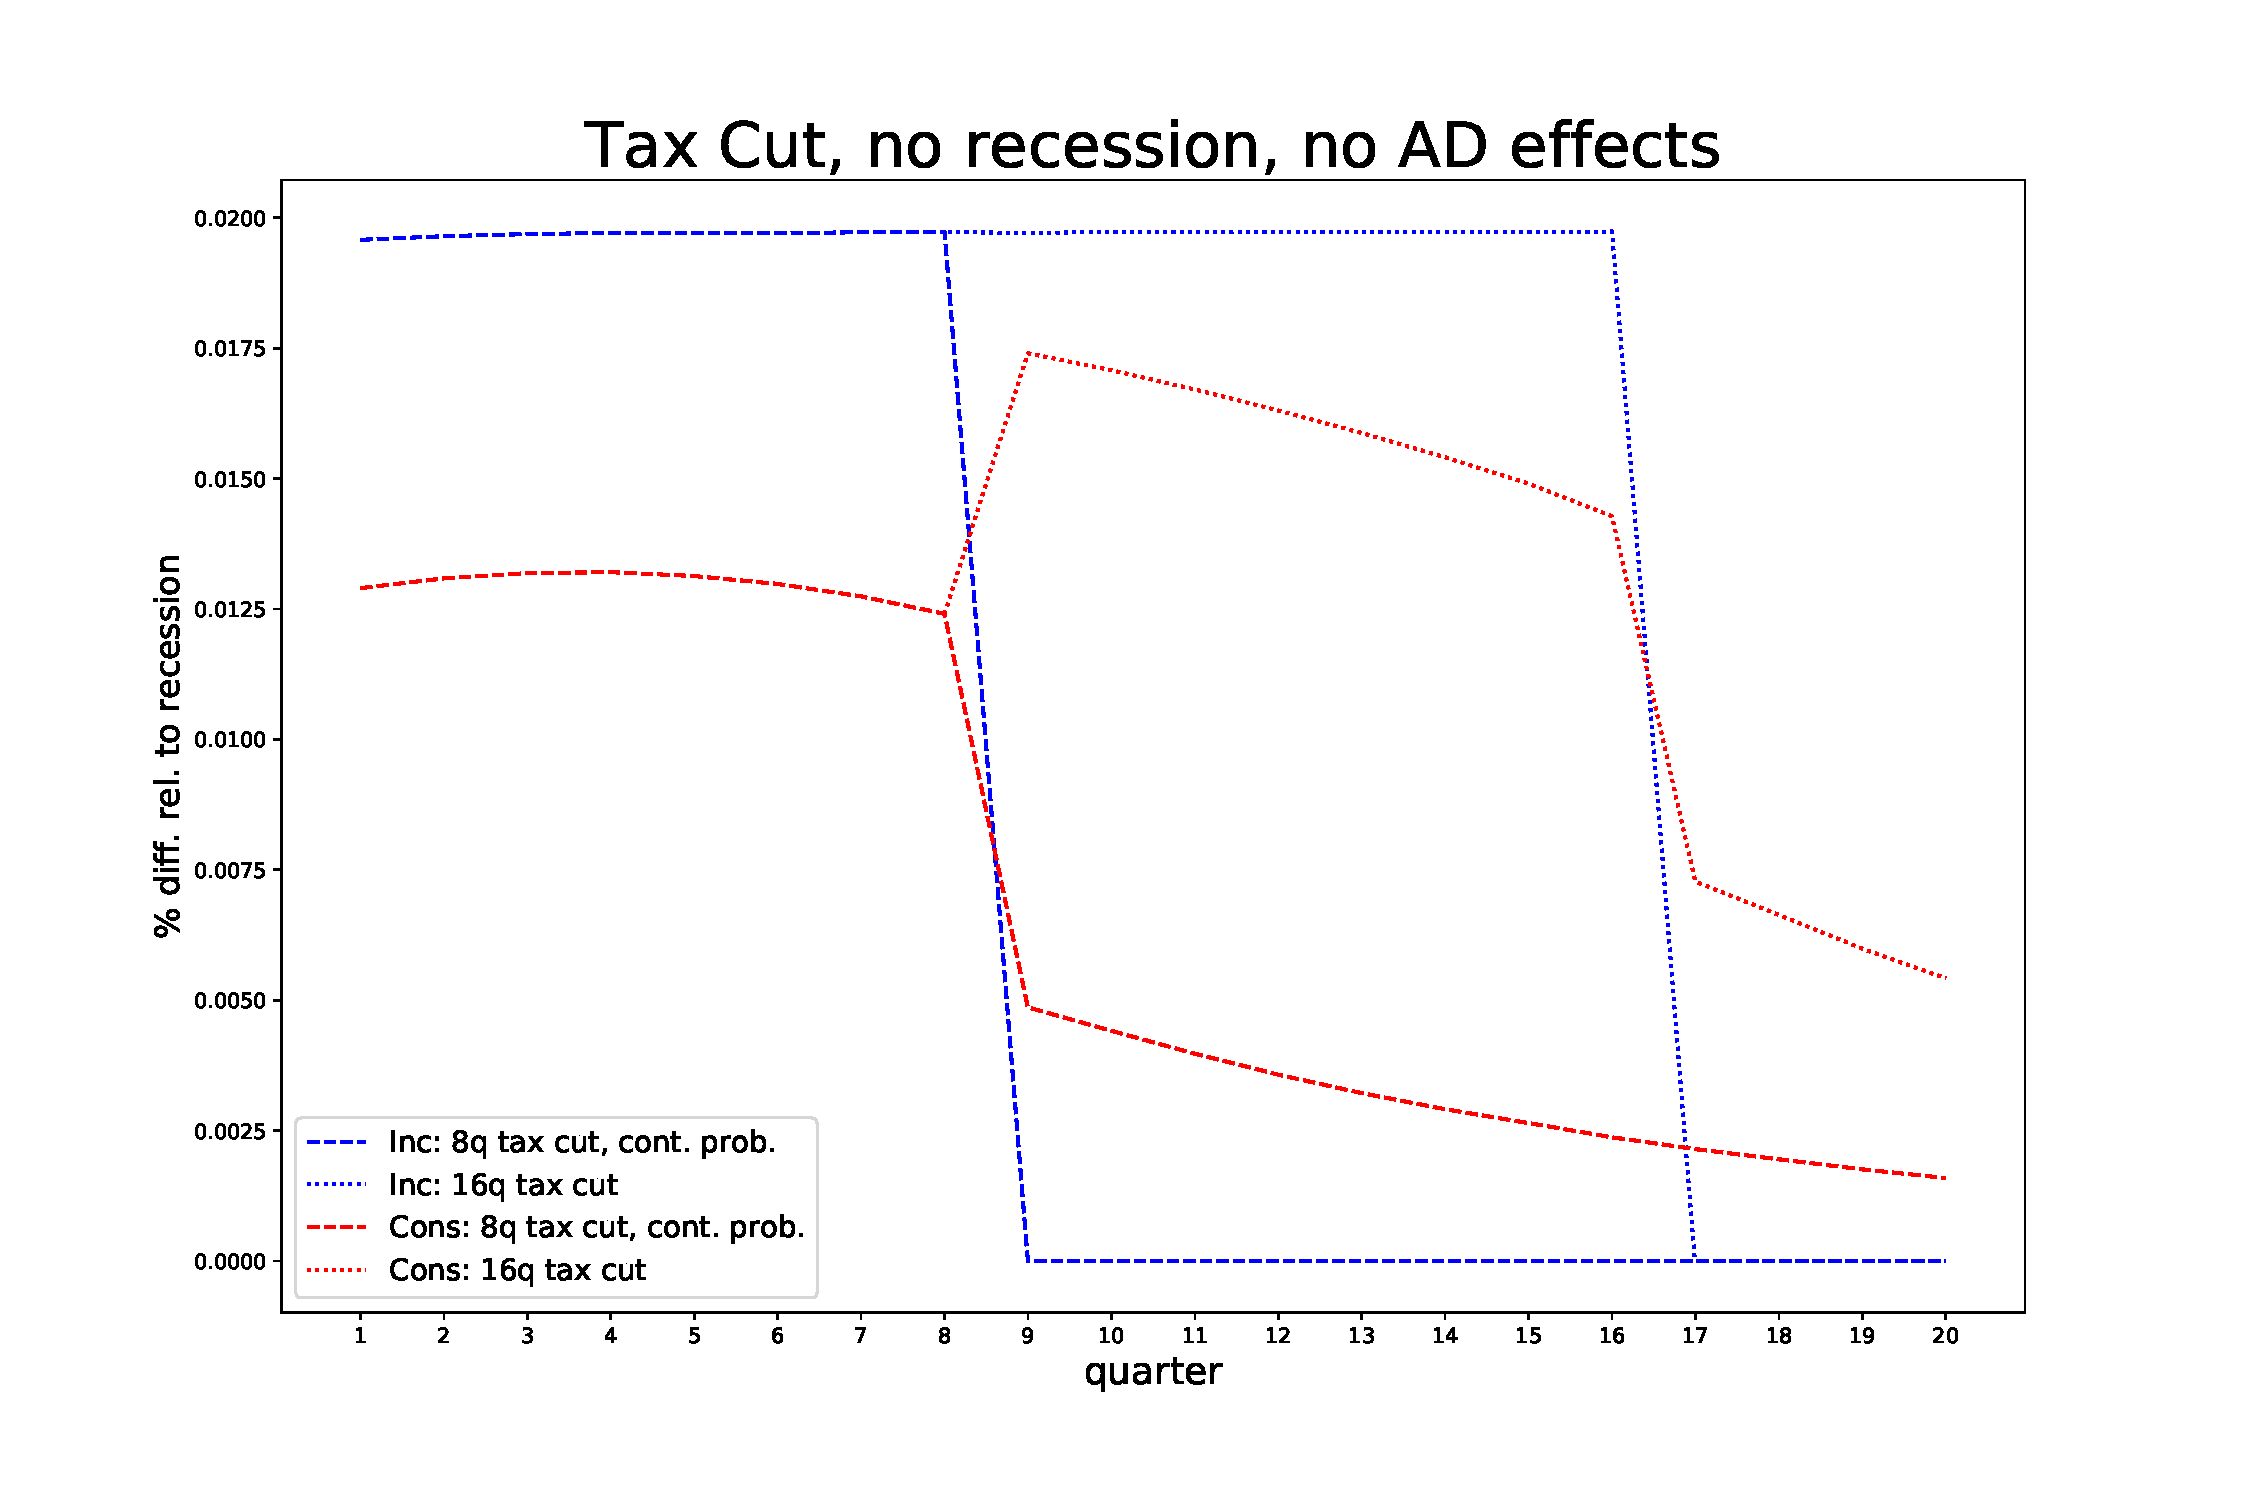
\includegraphics[width=\linewidth]{../Continuation_Prob_0/tax_cut_no_recession_no_AD_effects}
	\caption{}
	\label{fig:taxcutnorecessionnoadeffects}
\end{figure}

\begin{itemize}
	\item Figure \ref{fig:taxcutnorecessionadeffects} shows the payroll tax cut with AD effects
	\item Income increases for either 8 or 16 q depending on scenario. However, income now increase by more than 2\% percent because of AD effects, implying an additional boost to income when the continuation of the payroll tax cut is implemented.
\end{itemize}
	
\begin{figure}
	\centering
	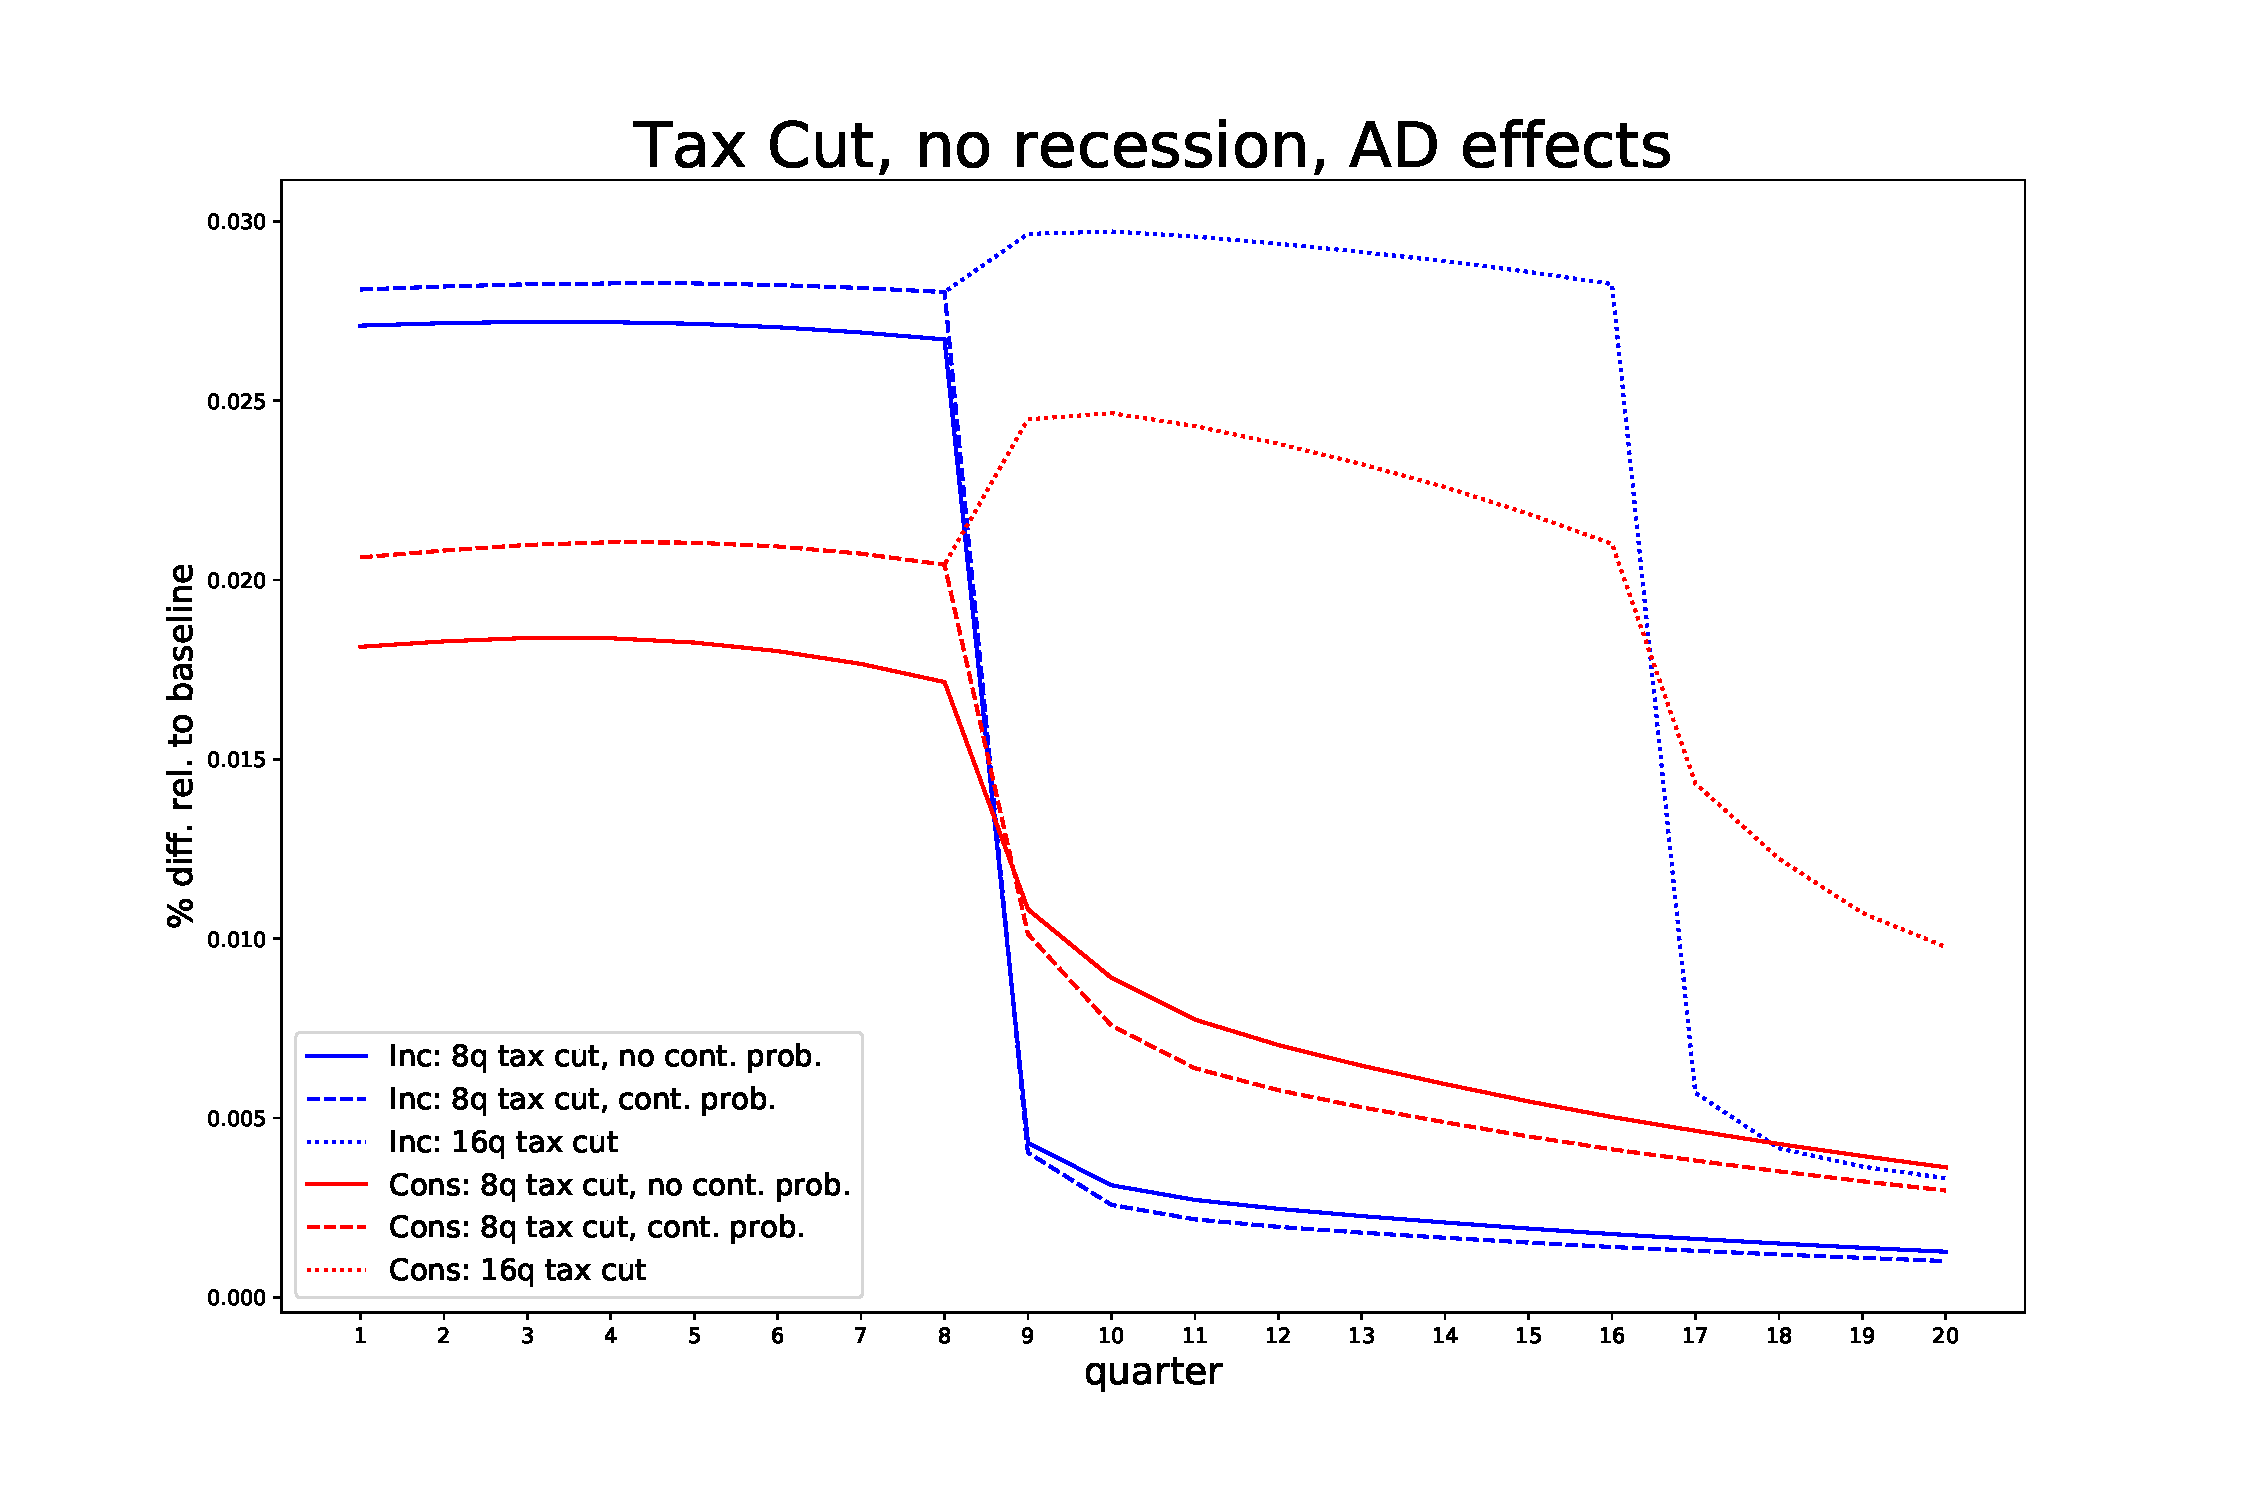
\includegraphics[width=\linewidth]{../Continuation_Prob_0/tax_cut_no_recession_AD_effects}
	\caption{}
	\label{fig:taxcutnorecessionadeffects}
\end{figure}



\FloatBarrier
\subsection{Sample size and speed of simulation}

In the following we test the speed of the code for solving and running the recession scenario. We assume that there is one discount factor common to all agents.

The following table shows the time needed to run the code, that i) solves the model without AD effects, ii) solves the model with AD effects and iii) simulates the considered scenario with and without AD effects.\footnote{40 simulations are performerd here, i.e. recessions that last 1 to 20q, with and without AD effects.} The second point requires solving the model several times repeadetly with macroeconmic beliefs of agents being updated in each iteration. For this reason, this step is by far the most time-intensive. When solving the model with AD effects, the algorithm is terminated when the change in beliefs from one to the next iteration falls below a certain tolerance. The second and third row of the table compare two different levels of that tolerance.\footnote{The change is measured as the Euclidean norm of the difference in slopes and intercepts of the linear function on the consumption ratio, which agents use to predict future income.} Note, that while solving with more agents is somewhat slower, it actually helps the algorithm to find the AD solution with fewer iterations. Simulating the larger number of agents is much slower, however.

\begin{center}
	\begin{tabular}{||c| c |c||} 
		\hline
		  & Sample 50k & Sample 200k \\ [0.5ex] 
		\hline\hline
		Solving without AD &  1 min & 1 min 20 sec  \\ \hline
		Solving with AD (tol: 1E-3) &  10 min ( 10 iter.)  & 12 min (7 iter.)  \\ \hline
		Solving with AD (tol: 1E-4) &  22 min ( 20 iter.)  & 16 min (10 iter.)  \\ \hline
		Simulation & 2 min 20 sec  & 16 min \\ [1ex] 
		\hline
	\end{tabular}
\end{center}

Figure \ref{fig:CRatio} plots $CR_t$ on  $CR_{t-1}$ where $CR_t$ is the ratio of simulated consumption to the baseline consumption in period $t$. The assumption behind our numerical algorithm to solve the model under AD effects is that individuals are able to predict the future consumption ratio, and thus their expected income (taking into account aggregate demand effects), based on a linear function of today's consumption ratio. If that assumption is correct, it should hold, that $CR_t = i + s (CR_{t-1} - 1 )$. Hence, we should see a line with a constant gradient. As seen in the figure, this only holds approximately. A higher sample size somewhat improves the picture, a lower tolerance value for the convergence of macro beliefs does not.

\begin{figure}
	\centering
	\begin{subfigure}[b]{0.45\textwidth}
		\centering
		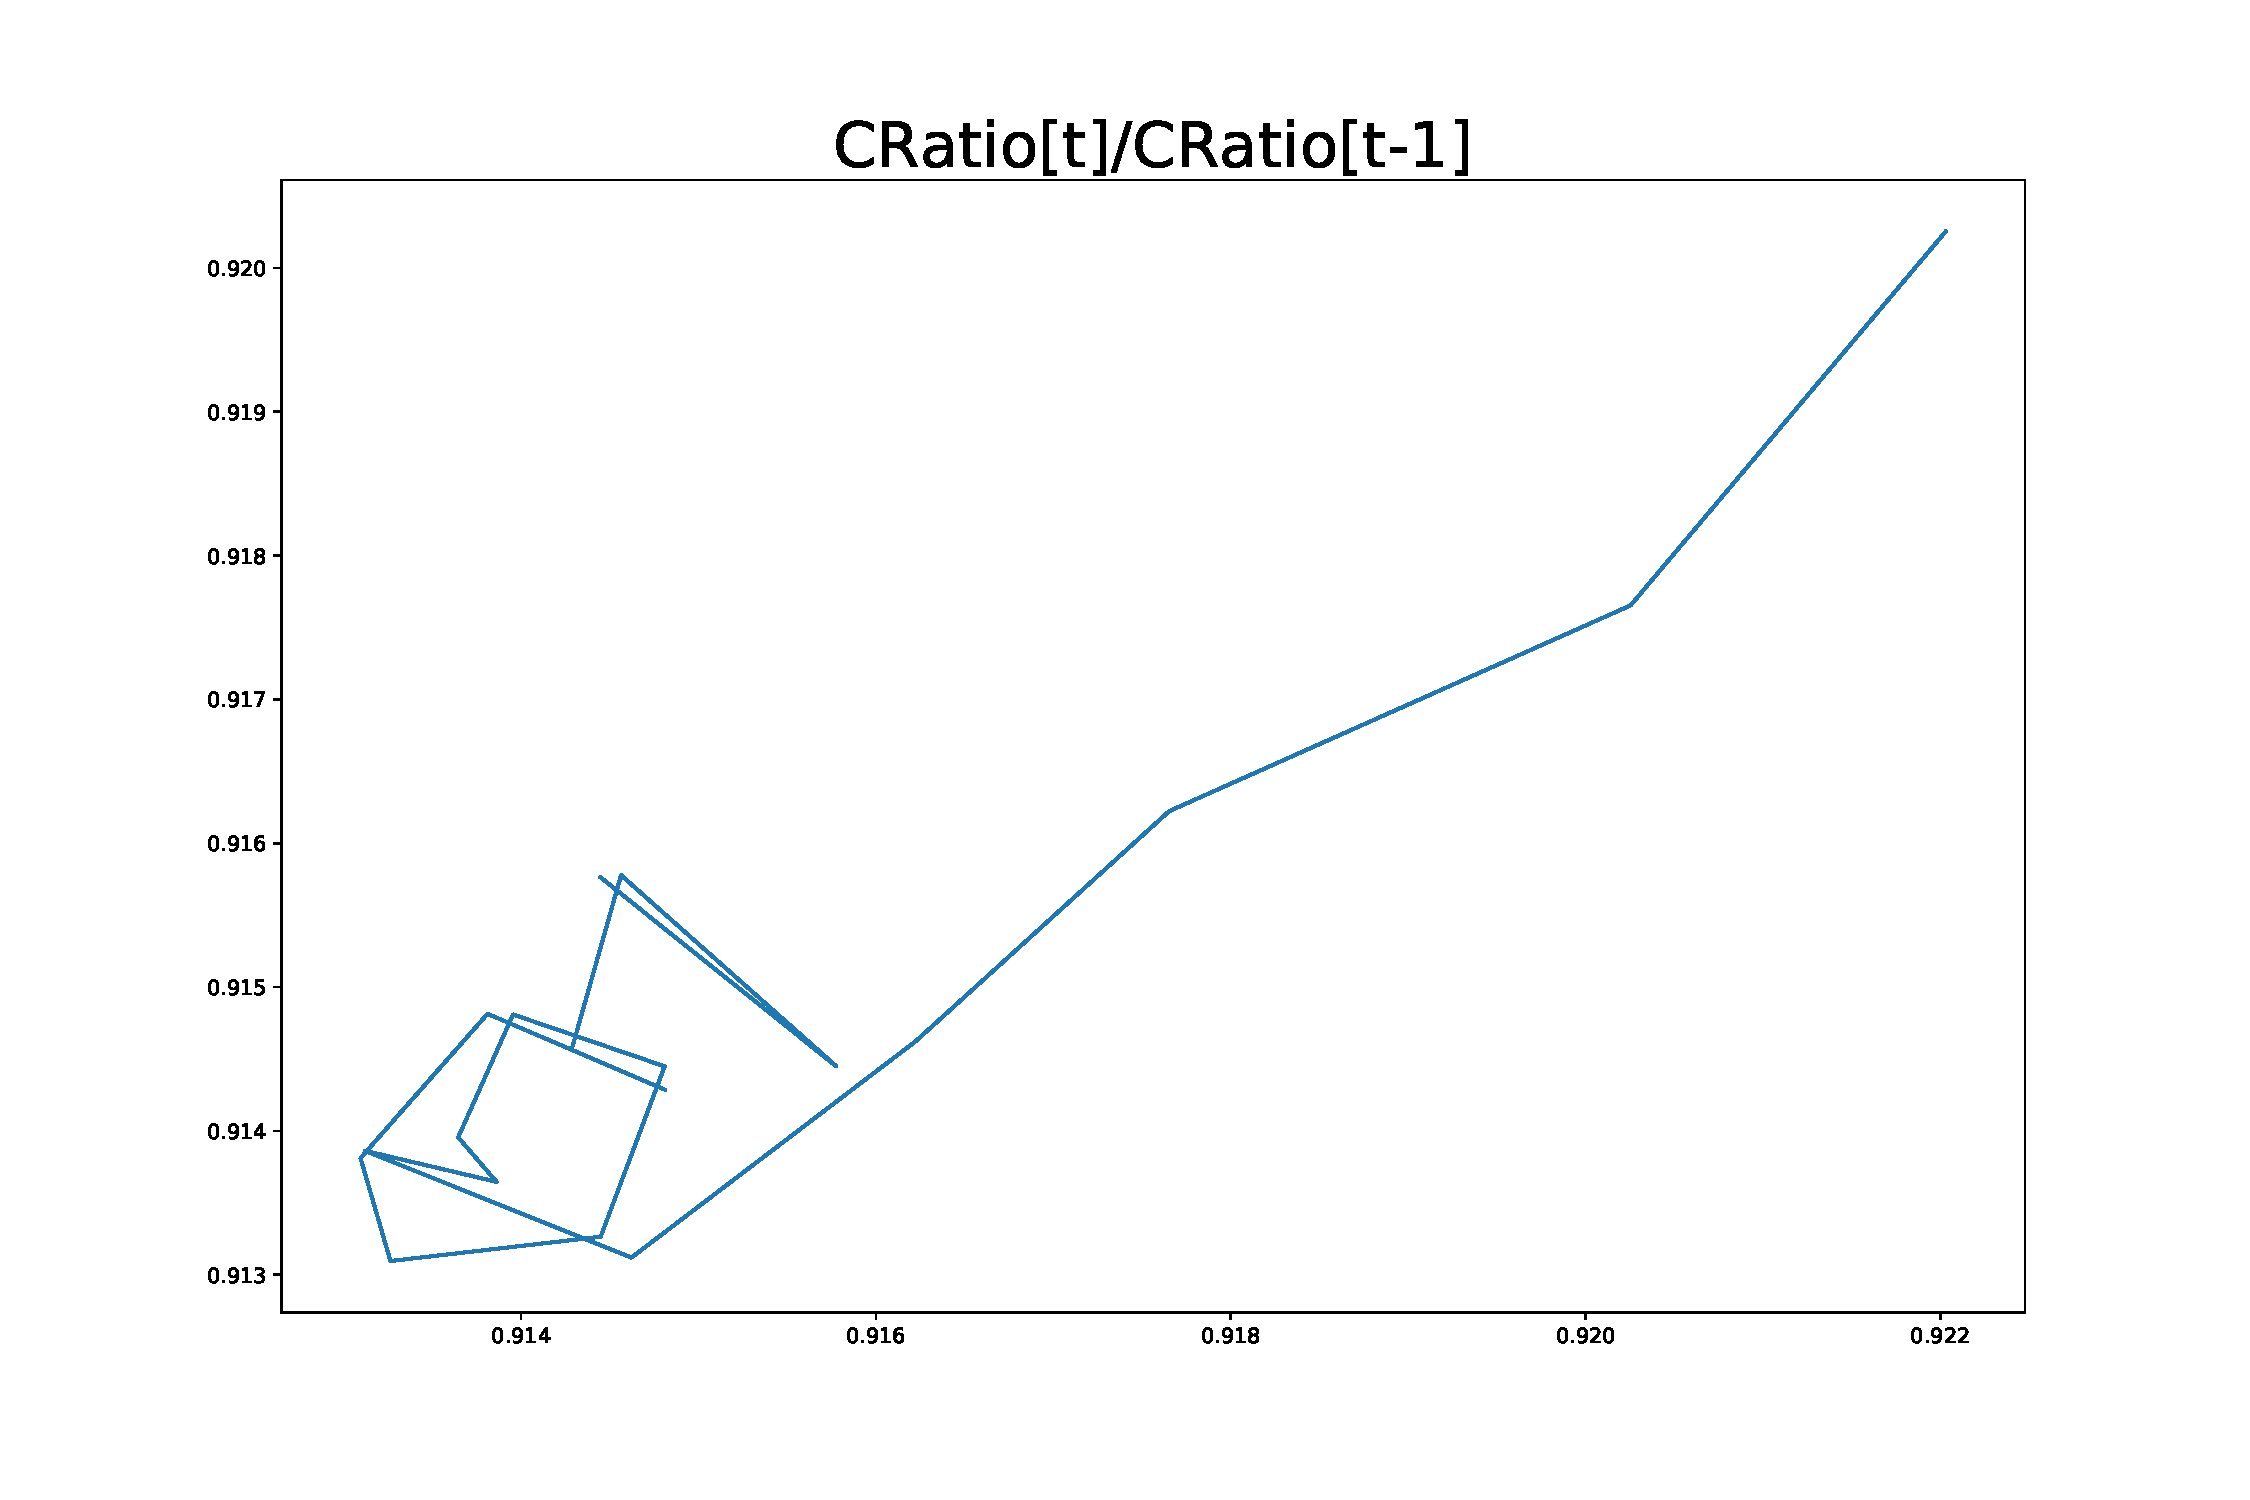
\includegraphics[width=1.2\textwidth]{../50kSample_BaseCal/CRatio.pdf}
		\caption{Sample 50k, tol = 1E-3}
		\label{fig:Cratio-50k-Baseline}
	\end{subfigure}
	\hfill
	\begin{subfigure}[b]{0.45\textwidth}
		\centering
		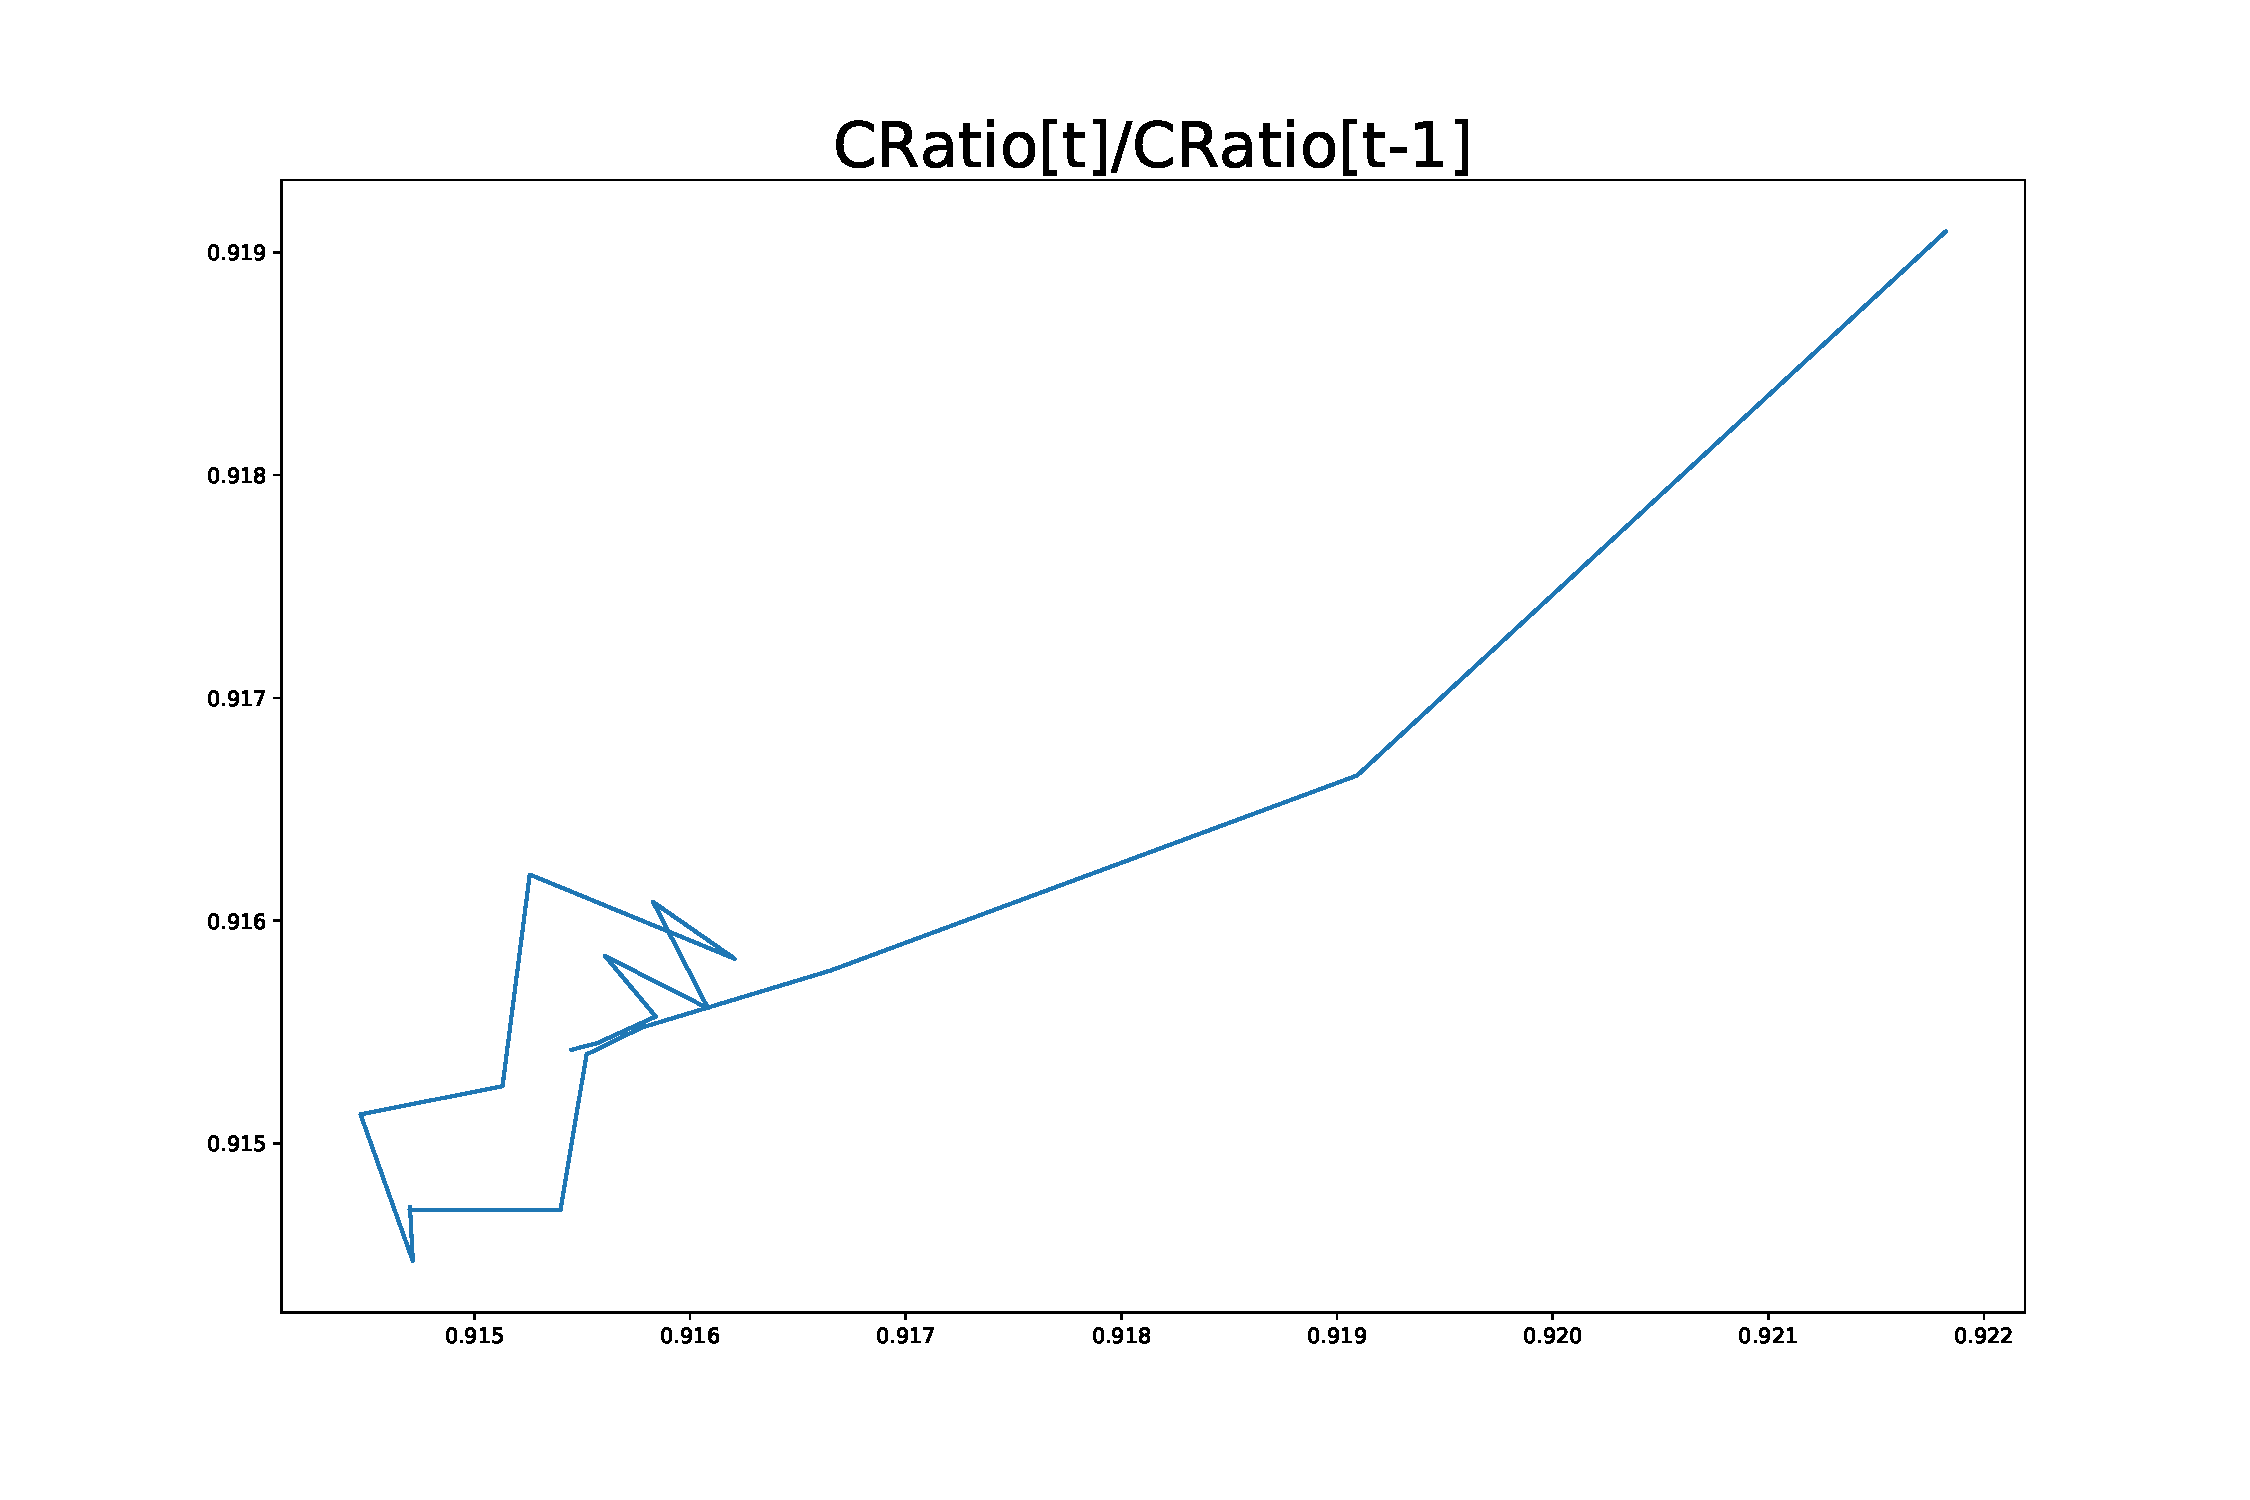
\includegraphics[width=1.2\textwidth]{../200kSample_BaseCal/CRatio.pdf}
		\caption{Sample 200k, tol = 1E-3}
		\label{fig:Cratio-200k-Baseline}
	\end{subfigure}\\
	\begin{subfigure}[b]{0.45\textwidth}
		\centering
		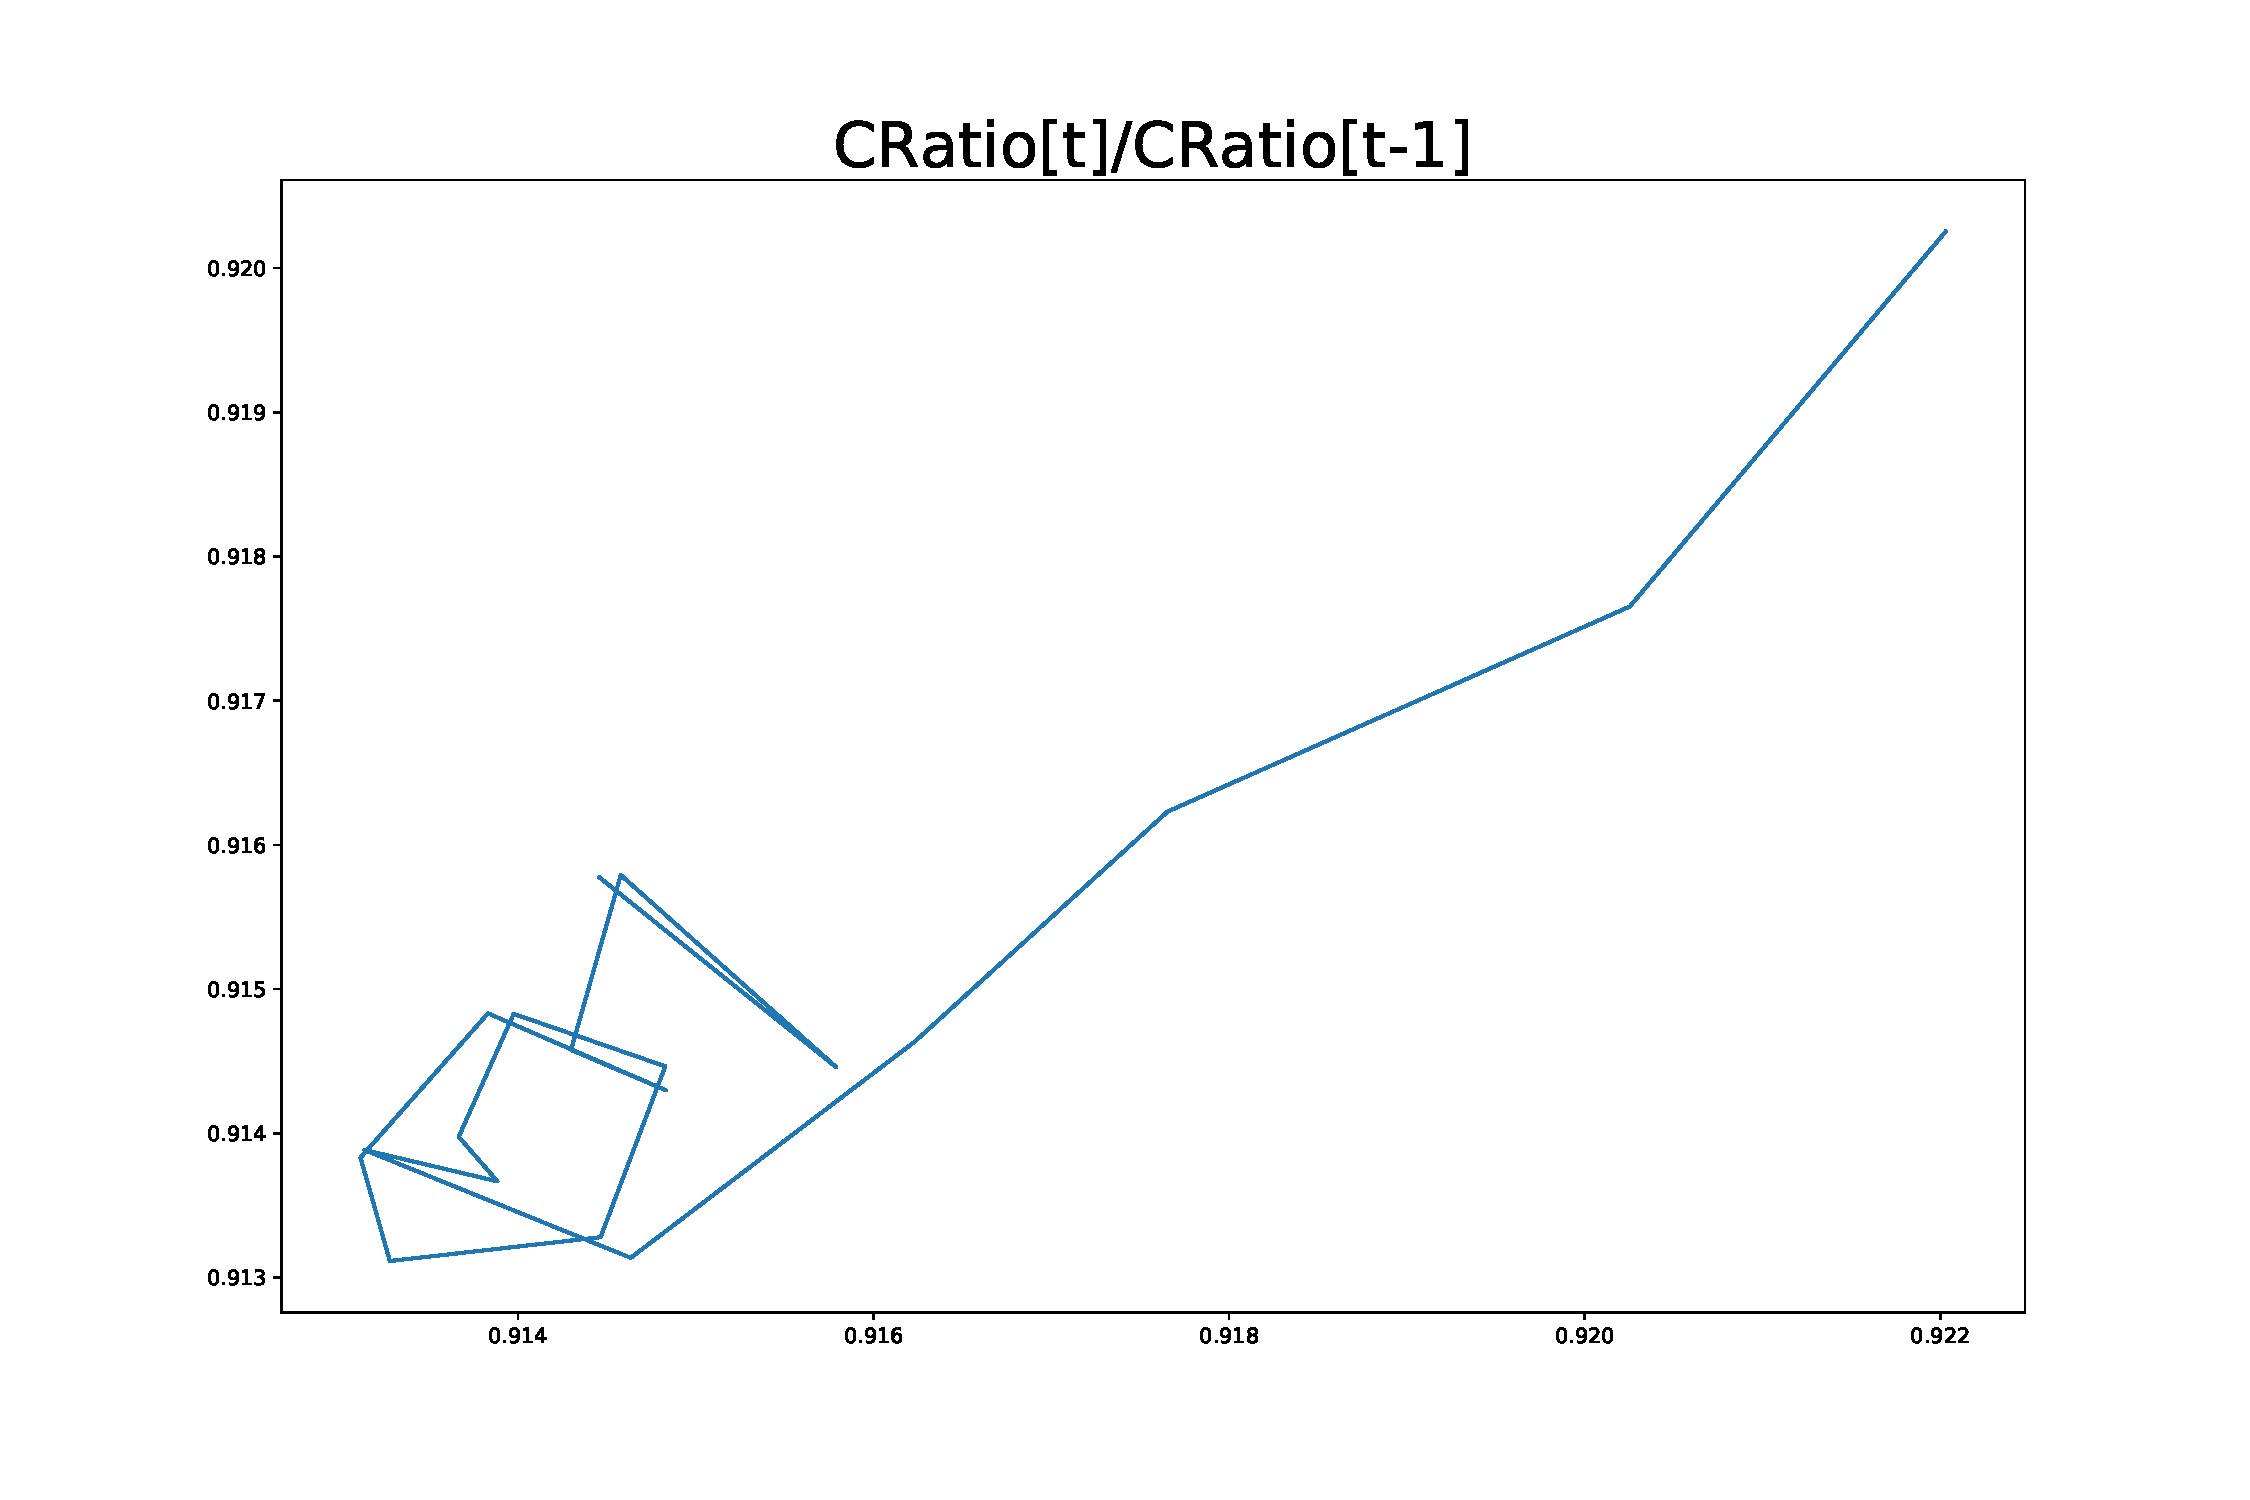
\includegraphics[width=1.2\textwidth]{../50kSample_BaseCal_TolE-4/CRatio.pdf}
		\caption{Sample 50k, tol = 1E-4}
		\label{fig:Cratio-50k}
	\end{subfigure}
	\hfill
	\begin{subfigure}[b]{0.45\textwidth}
		\centering
		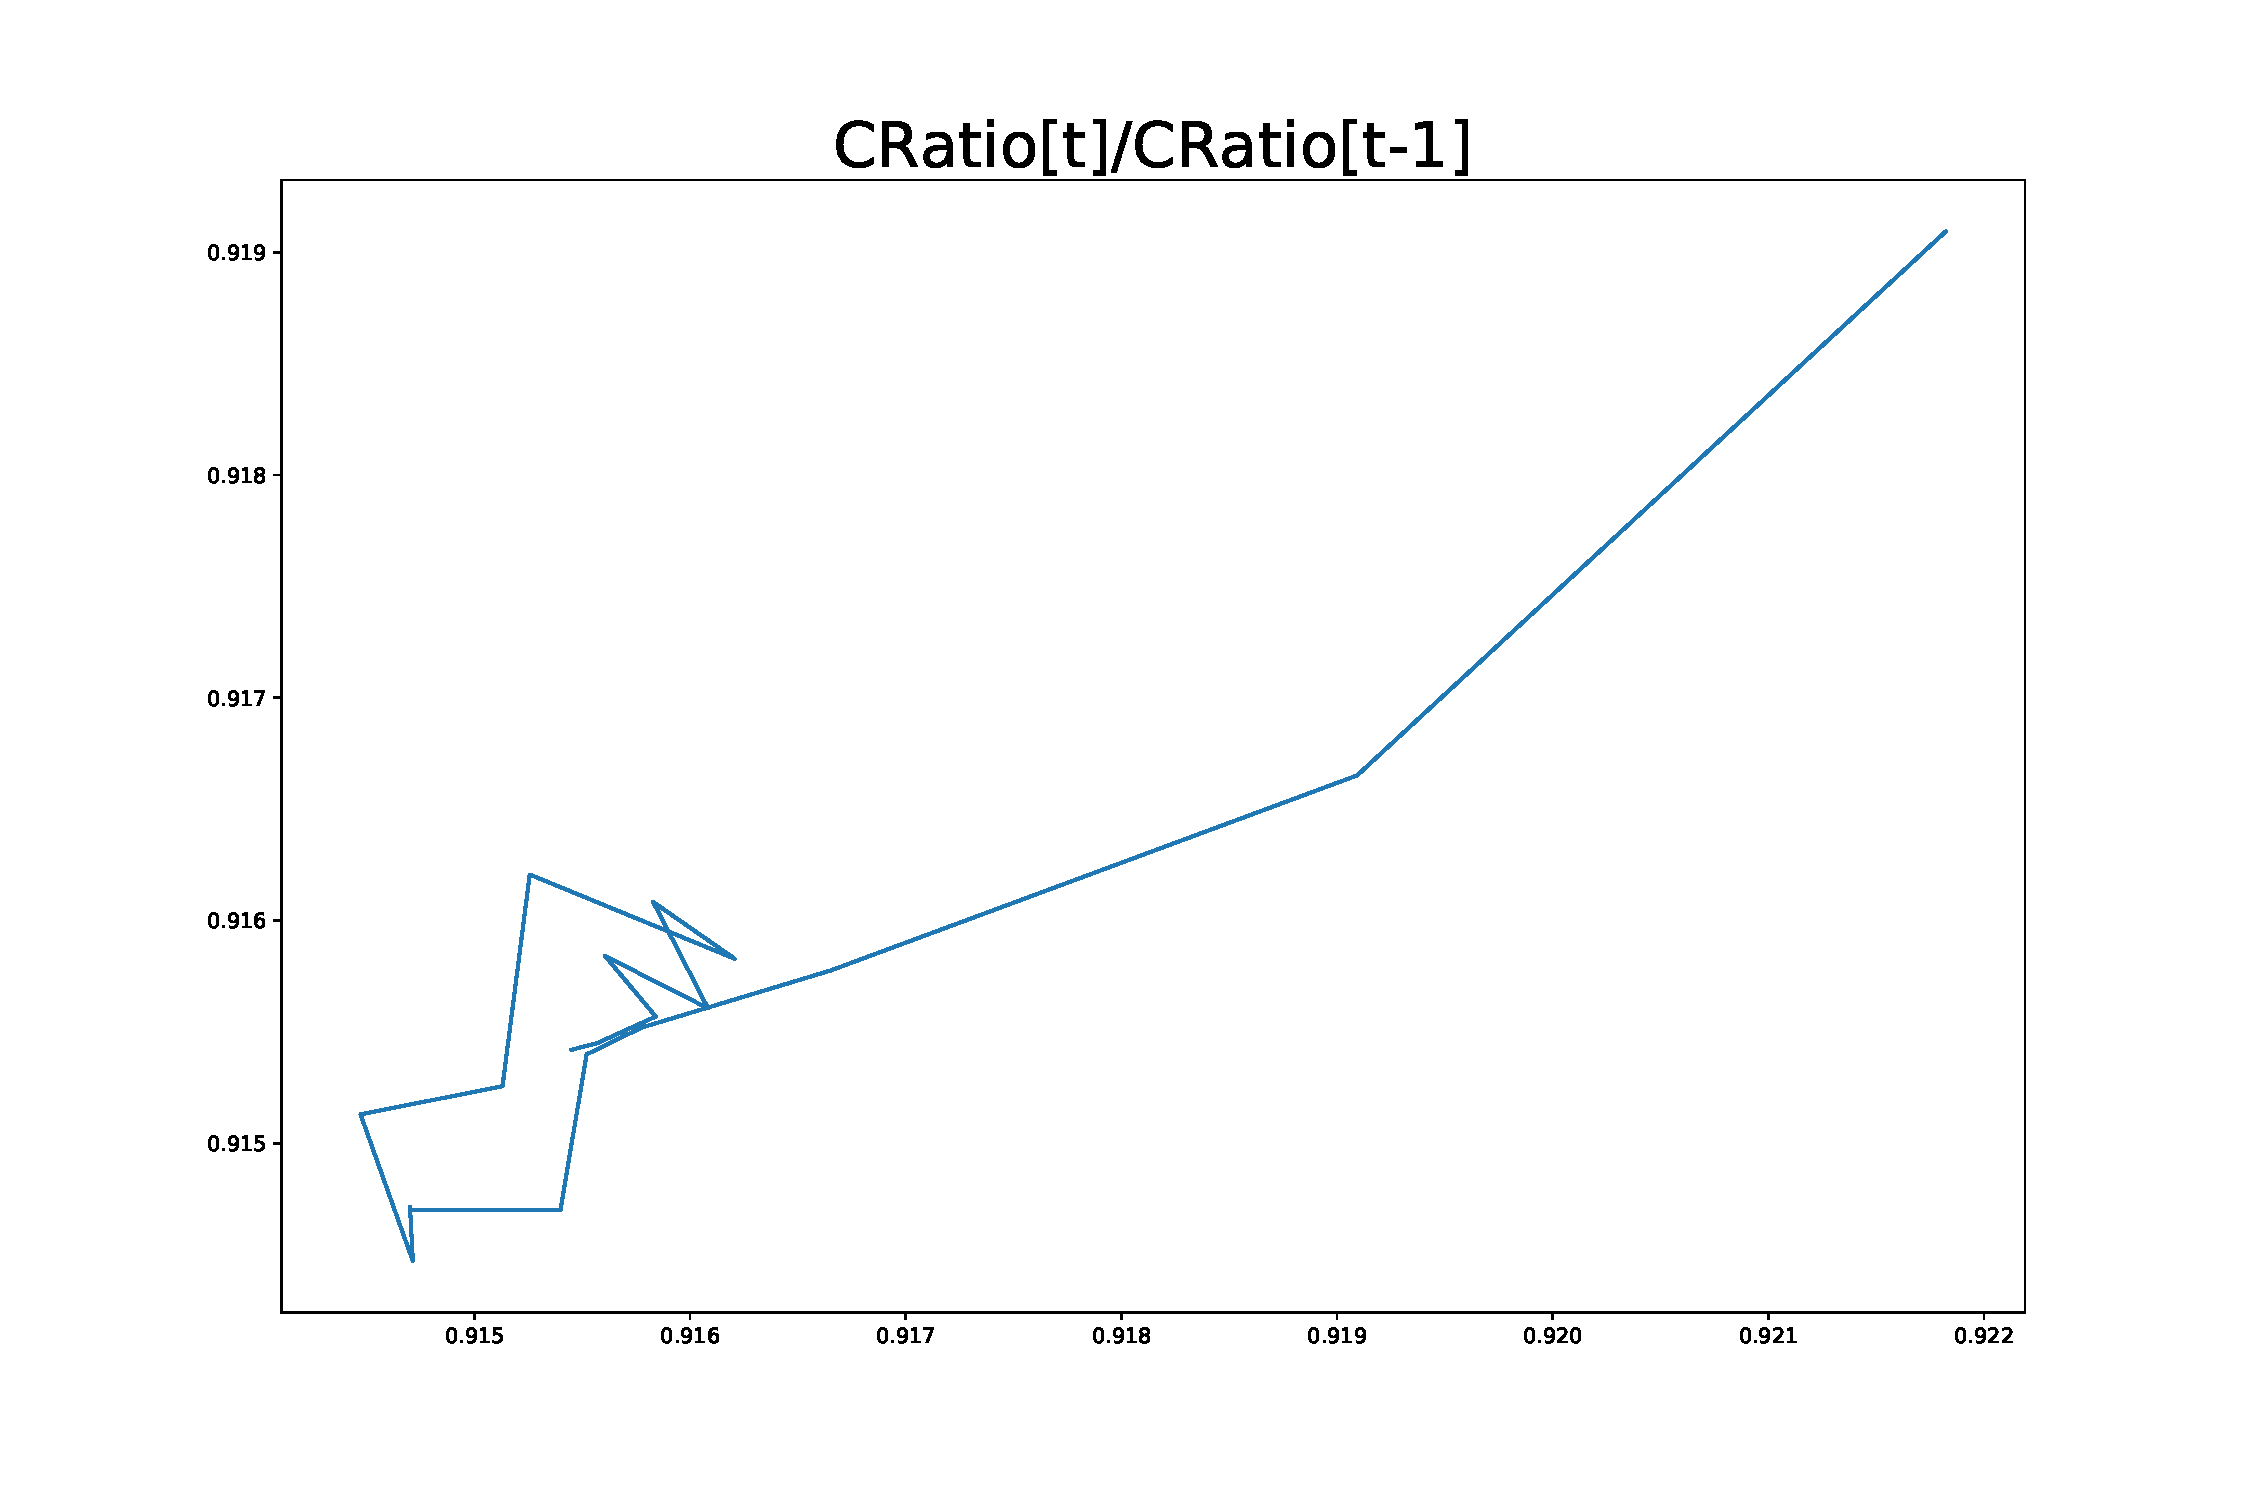
\includegraphics[width=1.2\textwidth]{../200kSample_BaseCal_TolE-4/CRatio.pdf}
		\caption{Sample 200k, tol = 1E-4}
		\label{fig:Cratio-200k}
	\end{subfigure}
	\caption{Plotting $CR_t$ (y-axis) on $CR_{t-1}$ (x-axis). (subfigure's title misleading, please ignore)}
	\label{fig:CRatio}
\end{figure}


\end{comment}





\end{document}
